% $Id: mpman.tex 524 2008-05-13 23:01:45Z stephanhennig $
% MetaPost manual, by John Hobby.  License at end.
\listfiles
\RequirePackage{ifpdf}
\ifpdf
\ifnum\pdftexversion<140
\else
\pdfminorversion=5
\pdfobjcompresslevel=1% Use compressed object streams.
\fi
\RequirePackage{cmap}
\fi
\documentclass{article} % article is NOT the original style
\usepackage[nofancy]{svninfo}% Access VCS information.
\svnInfo $Id: mpman.tex 524 2008-05-13 23:01:45Z stephanhennig $
\newcommand*{\mpversion}{1.005}

\usepackage[T1]{fontenc}
\usepackage{lmodern}
\usepackage{textcomp}
\usepackage{mflogo}
\usepackage{makeidx}
\usepackage{fancyvrb}
\usepackage{ctabbing}
\RecustomVerbatimEnvironment
  {verbatim}{BVerbatim}{baseline=c}
\usepackage{graphicx}
\usepackage[latin1]{inputenc}
\usepackage[textwidth=6in,textheight=8.65in]{geometry}
\usepackage{tocloft}
  \setlength\cftbeforesecskip{1.3ex plus 0.3ex minus 0.3ex}
\usepackage{ltxtable}


\def\ttindex#1{{\tt #1}\index{#1?\texttt{#1}}}
\def\ttt{\texttt}  % I get tired of typing this out

\def\ConTeXt{Con\TeX t}

\newcommand\descr[1]{{\langle\hbox{#1}\rangle}}
\newcommand\invisgap{\nobreak\hskip0pt\relax}
\newcommand\tdescr[1]{$\langle$\invisgap#1\invisgap$\rangle$}

\newcommand\pl{\dag}

\newcommand\mathcenter[1]{\vcenter{\hbox{#1}}}


\renewcommand{\topfraction}{.85}
\renewcommand{\bottomfraction}{.7}
\renewcommand{\textfraction}{.15}
\renewcommand{\floatpagefraction}{.5}
\renewcommand{\dbltopfraction}{.66}
\renewcommand{\dblfloatpagefraction}{.66}
\setcounter{topnumber}{9}
\setcounter{bottomnumber}{9}
\setcounter{totalnumber}{20}
\setcounter{dbltopnumber}{9}

\makeindex

\usepackage{multicol}
\usepackage[rgb,x11names]{xcolor}% Optimize for screen reading.
\usepackage{hyperxmp}
\usepackage{hyperref}
\hypersetup{
  pdftitle={A User's Manual for MetaPost},
  pdfauthor={John D. Hobby and the MetaPost development team},
  pdfkeywords={MetaPost, PostScript, vector graphics language, MetaFont, TeX}
}
\hypersetup{
  pdfstartview={XYZ null null null},% Zoom factor is determined by viewer.
  colorlinks,
  linkcolor=RoyalBlue3,
  urlcolor=Chocolate4,
  citecolor=SpringGreen3
}
\usepackage[all]{hypcap}
\ifpdf
\pdfmapfile{=cm2lm.map}% replace CM by LM in figures
\else
\DeclareGraphicsExtensions{.mps}
\DeclareGraphicsRule{mps}{eps}{*}{}
\usepackage{breakurl}
\fi
\begin{document}
\VerbatimFootnotes
%%% Title page layout documentation is missing.
\begin{titlepage}
  \vbox to \textheight {%
    \vskip0pt
    \vfil
    \vfil
    \vfil
    \centerline{\resizebox{3.5in}{!}{\fontseries{b}\selectfont\MP}}
    \vskip10bp% actually 21bp (-11bp)
    \centerline{\includegraphics{manfig-60.mps}}
    \vskip15bp% actually 21bp (-6bp)
    \centerline{%
      \resizebox{3.5in}{!}{%
        \scshape%
        \fontsize{28bp}{28bp}\selectfont
        \strut\lowercase{A USER\kern-2bp\lower3bp\hbox{'}S MANUAL}%
      }%
    }
    \vskip-11bp
    \vfil
    \vfil
    \centerline{\large John D. Hobby}
    \vskip3bp
    \centerline{and the MetaPost development team}
    \vskip20.8bp% actually 31.8bp (-11bp)
    \centerline{\large documented version: \mpversion}
    \vskip3bp
    \centerline{\svnToday}
    \vfil
    \vfil
    \vfil
  }
\end{titlepage}

\setlength{\columnsep}{2.5em}
\begin{multicols}{2}
\tableofcontents
\end{multicols}

\section{Introduction}
\label{intro}

MetaPost is a programming language much like Knuth's \MF\footnote{\MF\
is a trademark of Addison Wesley Publishing
company.}\index{metafont?\MF}~\cite{kn:c} except that it outputs
PostScript programs instead of bitmaps.  Borrowed from \MF\ are the
basic tools for creating and manipulating pictures. These include
numbers, coordinate pairs, cubic splines, affine transformations, text
strings, and boolean quantities.  Additional features facilitate
integrating text and graphics and accessing special features of
PostScript\footnote{PostScript is a trademark of Adobe Systems
Inc.}\index{PostScript} such as clipping, shading, and dashed lines.
Another feature borrowed from \MF\ is the ability to solve linear
equations that are given implicitly, thus allowing many programs to be
written in a largely declarative style.  By building complex operations
from simpler ones, MetaPost achieves both power and flexibility.

MetaPost is particularly well-suited to generating figures for technical
documents where some aspects of a picture may be controlled by
mathematical or geometrical constraints that are best expressed
symbolically.  In other words, MetaPost is not meant to take the place
of a freehand drawing tool or even an interactive graphics editor.  It
is really a programming language for generating graphics, especially
figures for \TeX\footnote{\TeX\ is a trademark of the American
Mathematical Society.}\index{TeX?\TeX} and troff\index{troff} documents.

To use MetaPost, you prepare an input file containing MetaPost code and
then invoke MetaPost, usually by giving a command of the
form\index{mpost?\texttt{mpost}}
$$ {\tt mpost}\, \descr{filename} $$
The syntax and program name itself are system-dependent; sometimes it is
named \texttt{mp}.  MetaPost input
files\index{files!input} normally have names ending ``{\tt .mp}'' but
this part of the name can be omitted when invoking MetaPost.  For an
input file {\tt foo.mp}
$$ \hbox{\tt mpost foo} $$
invokes MetaPost and produces output files with names like {\tt foo.1}
and {\tt foo.2}.  Any terminal I/O is summarized in a
transcript\index{files!transcript}\index{transcript file} file called
{\tt foo.log}.  This includes error messages and any MetaPost commands
entered interactively.\footnote{A {\tt *}\index{*?\texttt{*}} prompt is
used for interactive input and a {\tt **}\index{**?\texttt{**}} prompt
indicates that an input file name is expected.  This can be avoided by
invoking MetaPost on a file that ends with an {\tt
end}\index{end?\texttt{end}} command.} 

\label{Dmpversion}The transcript file starts with a banner line that
identifies the version of MetaPost you are using.  You can also determine
the current version from within a MetaPost program via the
\texttt{mpversion} predefined constant string (this was introduced in
version 0.9).  For instance:
$$\begin{verbatim}
if known mpversion:
  message "mp = " & mpversion;
  if scantokens(mpversion) < 1: message "CMYK color support not available!" fi
fi
\end{verbatim}
$$
prints
$$\begin{verbatim}[commandchars=\\\{\}]
mp = \mpversion
\end{verbatim}
$$
The {\tt scantokens} command is described on p.~\pageref{Dscantokens}
and can be utilized to convert strings to numbers.
\index{Creator comment in PostScript output}%
The version number is also included in the \texttt{Creator} comment in
the PostScript output.

This document introduces the MetaPost language, beginning with the
features that are easiest to use and most important for simple
applications.  Reading the manual does not require knowledge of \MF\ or
access to {\sl The \MF book}, but both are beneficial.
The first few sections describe the language as it
appears to the novice user with key parameters at their default values.
Some features described in these sections are part of a predefined macro
package called Plain.  Later sections summarize the complete language
and distinguish between primitives and preloaded macros from the Plain
macro package\index{Plain macros}.  Since much of the language is
identical to Knuth's \MF, the appendix gives a detailed comparison so
that advanced users can learn more about MetaPost by reading {\sl The
\MF book\/} \cite{kn:c}.

MetaPost documentation is completed by ``Drawing Boxes with MetaPost''
and ``Drawing Graphs with MetaPost''---the manuals of the \texttt{boxes}
and \texttt{graph} packages originally developed by John~D. Hobby.

The MetaPost home page is \url{http://tug.org/metapost}.  It has links
to much additional information, including many articles that have been
written about MetaPost.  For general help, try the
\url{metapost@tug.org} mailing list; you can subscribe to this list at
\url{http://tug.org/mailman/listinfo/metapost}.

The development is currently hosted at
\url{https://foundry.supelec.fr/projects/metapost/}; visit this site
for the current development team members, sources, and much else.

Please report bugs and request enhancements either on the
\url{metapost@tug.org} list, or through the address given above.
(Please do not send reports directly to Dr.\ Hobby any more.)


\section{Basic Drawing Statements}
\label{basic}

The simplest drawing statements are the ones that generate straight lines.
Thus\index{draw?\texttt{draw}}\index{-{}-?\texttt{-{}-}}
$$ \hbox{\verb|draw (20,20)--(0,0)|} $$
draws\index{draw?\texttt{draw}} a diagonal line and
$$ \hbox{\verb|draw (20,20)--(0,0)--(0,30)--(30,0)--(0,0)|} $$
draws a polygonal line like this:
$$ \includegraphics{manfig-1} $$

\label{Ddrawdot}MetaPost also has a \ttt{drawdot} command to print a
single point, as in \ttt{drawdot(30,0)}. 

What is meant by coordinates like \verb|(30,0)|?  MetaPost uses the same
default coordinate system that PostScript\index{PostScript!coordinate
system} does.  This
means that \verb|(30,0)| is 30 units to the right of the origin, where a
unit is $1\over72$ of an inch.  We shall refer to this default unit as a
{\sl PostScript point\/}\index{PostScript!point}\index{point!PostScript}
to distinguish it from the standard printer's
point\index{point!printer's} which is $1\over72.27$ inches.

MetaPost uses the same names for units of measure that \TeX\ and \MF\
do.  Thus \verb|bp|\index{bp?\texttt{bp}}\label{Dbp} refers to
PostScript points (``big points'') and
\verb|pt|\index{pt?\texttt{pt}}\label{Dpt} refers to printer's points.
Other units of measure include
\verb|in|\index{in?\texttt{in}}\label{Din} for inches,
\verb|cm|\index{cm?\texttt{cm}}\label{Dcm} for centimeters, and
\verb|mm|\index{mm?\texttt{mm}}\label{Dmm} for millimeters.  For
example,
$$ \hbox{\verb|(2cm,2cm)--(0,0)--(0,3cm)--(3cm,0)--(0,0)|} $$
generates a larger version of the above diagram.  It is OK to say
\verb|0| instead \verb|0cm| because {\tt cm} is really just a conversion
factor and {\tt 0cm} just multiplies the conversion factor by zero.
(MetaPost understands constructions like {\tt
2cm}\index{multiplication, implicit} as shorthand for \verb|2*cm|).

It is convenient to introduce your own scale factor, say $u$.  Then you
can define coordinates in terms of $u$ and decide later whether you want
to begin with \verb|u=1cm| or \verb|u=0.5cm|.  This gives you control
over what gets scaled and what does not so that changing $u$ will not
affect features such as line widths.

There are many ways to affect the appearance of a line besides just
changing its width, so the width-control mechanisms allow a lot of
generality that we do not need yet.  This leads to the strange looking
statement\index{pickup?\texttt{pickup}}\index{pencircle?\texttt{pencircle}}%
\index{scaled?\texttt{scaled}}
$$ \hbox{\verb|pickup pencircle scaled 4pt|} $$
for setting the line width for subsequent \verb|draw| statements to 4 points.
(This is about eight times the default line width).

With such a wide line width, even a line of zero length comes out as a big bold
dot\index{dots}.  We can use this to make a grid of bold dots by having one
\verb|drawdot| statement
for each grid point.  Such a repetitive sequence of \verb|draw| statements is
best written as a pair of nested loops:\index{loops}%
\index{for?\texttt{for}}\index{endfor?\texttt{endfor}}
$$\begin{verbatim}
for i=0 upto 2:
  for j=0 upto 2:  drawdot (i*u,j*u);  endfor
endfor
\end{verbatim}
$$
The outer loop runs for $i=0,1,2$ and the inner loop runs for $j=0,1,2$.
The result is a three-by-three grid of bold dots as shown in Figure~\ref{fig1}.
The figure also includes a larger version of the polygonal line diagram that we
saw before.

\begin{figure}[htp]
$$ \begin{verbatim}
beginfig(2);
u=1cm;
draw (2u,2u)--(0,0)--(0,3u)--(3u,0)--(0,0);
pickup pencircle scaled 4pt;
for i=0 upto 2:
  for j=0 upto 2:  drawdot (i*u,j*u);  endfor
endfor
endfig;
\end{verbatim}
\quad \mathcenter{\includegraphics{manfig-2}}
$$
\caption{MetaPost commands and the resulting output}
\label{fig1}
\end{figure}

Note that the program in Figure~\ref{fig1} starts with
\verb|beginfig(2)|\index{beginfig?\texttt{beginfig}} and ends with
\verb|endfig|\index{endfig?\texttt{endfig}}.  These are macros that
perform various administrative functions and ensure that the results of
all the \verb|draw| statements get packaged up and translated into
PostScript.  A MetaPost input file normally contains a sequence of
\verb|beginfig|, \verb|endfig| pairs with an {\tt
end}\index{end?\texttt{end}} statement after the last one.  If this file
is named {\tt fig.mp}, the output from \verb|draw| statements between
\verb|beginfig(1)| and the next \verb|endfig| is written in a file {\tt
fig.1}\index{files!output}.  In other words, the numeric argument to the
\verb|beginfig| macro determines the name of the corresponding output
file.

What does one do with all the PostScript files?  They can be included as
figures in a \TeX\index{TeX?\TeX} or troff\index{troff} document if you
have an output driver that can handle encapsulated PostScript figures.
They can also be previewed before they are included in a thousand pages
document.  The next sections give some more information.


\section{Handling MetaPost output}
\label{Dmpoutput}

There can be a two-fold interaction between \TeX\ and MetaPost.  On one
hand, MetaPost graphics can be imported into documents typeset by \TeX\
and friends.  On the other hand, MetaPost can delegate typesetting
textual elements to \TeX, \LaTeX\ or \emph{troff}, e.g., text labels or
mathematical formulas in a graphic.  That way, MetaPost graphics can
easily adopt the style of a document (type, type size, etc.) and fit its
typesetting quality (use kerning, ligatures, etc.)  This makes MetaPost
an ideal tool for preparing high-quality graphics for \TeX\ or
\emph{troff} documents.

This section deals with the first aspect of \TeX--MetaPost interaction,
the import of MetaPost graphics into \TeX\ and friends.  Typesetting
text in MetaPost is discussed in section~\ref{text}.


\subsection{Previewing MetaPost graphics}
\label{Dpreview}
\index{previewing}

The output of MetaPost is a variant of PostScript, called Encapsulated
PostScript\index{PostScript!structured} (EPSF\index{EPSF}).  MetaPost
graphics can therefore be previewed with any decent PostScript viewer,
e.\,g., GSview\index{GSview}.

The situation becomes only a little bit fussy when MetaPost output
contains text.  By default, MetaPost doesn't produce self-contained EPS
files, e.\,g., font resources and encoding vectors are not stored in
the output.  For that reason MetaPost output containing text may be
rendered with wrong fonts, wrong glyphs or with no text at all in a
PostScript viewer.  For a long time, the most reliable way for
previewing was to prepare a test document that includes all MetaPost
figures, process that with \TeX\ or \LaTeX\ and \ttindex{dvips} and
display the resulting \ttt{ps} file in a PostScript
viewer.\footnote{There are alternatives, though. \ttindex{mpstoeps} is
a Perl script that automates the process outlined above.
\ttindex{mptopdf} is another tools that converts MetaPost files to
PDF.}

However, with MetaPost version~1.000 the situation changed.  Since that
version MetaPost is able to produce self-contained EPS files, that can
reliably be previewed, may they contain text or not.  The
new behaviour can be triggered by setting MetaPost's internal variable
\ttt{prologues}\index{prologues?\texttt{prologues}} to~3.  See
section~\ref{Dbtex} for more information on \ttt{prologues}.


\subsection{Using MetaPost graphics in \TeX, \LaTeX, pdf\LaTeX, pdf\TeX, Con\TeX{}t and troff}
\label{Dteximport}
\index{TeX?\TeX!importing MetaPost files}
\index{LaTeX?\LaTeX!importing MetaPost files}
\index{pdfLaTeX?pdf\LaTeX!importing MetaPost files}
\index{pdfTeX?pdf\TeX!importing MetaPost files}
\index{ConTeXt?Con\TeX t!importing MetaPost files}
\index{troff!importing MetaPost files}

How MetaPost figures can be integrated into documents prepared with
\TeX\ and friends depends on the exact format and output driver.
Figure~\ref{fig0} shows the workflow for plain \TeX, \LaTeX\ and the
freely available program \ttindex{dvips}.\footnote{The C source for
\ttt{dvips} comes with the web2c \TeX\ distribution.  Similar programs
are available from other sources.}  A similar procedure works with
troff: the \ttt{grops} output processor includes PostScript figures when
they are requested via troff's \ttt{\string\X} command.  For the PDF
flavour of \TeX\ and \LaTeX\ the situation is a little bit different.
The next paragraphs give brief information on some popular \TeX\ formats
and output drivers.

\begin{figure}[htp]
$$ \includegraphics{manfig-0} $$
\caption[A diagram of the processing for a document with MetaPost figures]
        {A diagram of the processing for a \TeX\ document with figures
        in MetaPost}
\label{fig0}
\end{figure}

\paragraph{\TeX}
\TeX\ users can import EPS graphics by first loading package
\ttt{epsf}\index{epsf.tex?\texttt{epsf.tex}} via \verb+\input epsf+ and
then issuing the command
$$ \verb+\epsfbox{+\descr{filename}\verb+}+ $$%
\index{epsfbox?\texttt{\string\epsfbox}}
to load an EPS file, e.\,g., \verb+\epsfbox{fig.1}+.

\paragraph{\LaTeX}
For \LaTeX\ documents the procedure is similar:  first package
\ttindex{graphicx} has to be loaded by putting
\verb+\usepackage{graphicx}+ into the document preamble and then EPS
files can be loaded via
$$ \verb+\includegraphics{+\descr{filename}\verb+}+ $$%
\index{includegraphics?\texttt{\string\includegraphics}}
e.\,g., \verb+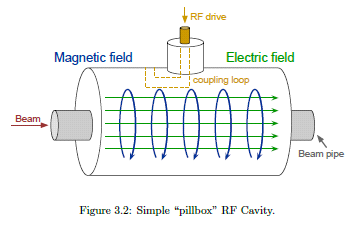
\includegraphics{fig.1}+.

As can be seen in figure~\ref{fig0} graphic files are never included in a
\TeX\index{TeX?\TeX!importing MetaPost files} or
\LaTeX\index{LaTeX?\LaTeX!importing MetaPost files} run.  Instead,
\TeX\ and \LaTeX\ only read bounding box information off PostScript
files, reserve as much space on a page as a graphic occupies and write
a reference to the corresponding file into \ttt{dvi} output.  Graphic
files are only included in the subsequent run of an output driver,
that can handle PostScript files, e.\,g., \ttindex{dvips}.

\paragraph{pdf\LaTeX}
The application pdf\LaTeX, when run in PDF mode, is both, a
\LaTeX\ interpreter and an output driver for the PDF document format.
For that reason graphic files are included in a single
pdf\LaTeX\ run.  In contrast to \ttt{dvips}, pdf\LaTeX\ can't process
general PostScript files, but only so-called purified
EPS\index{PostScript!purified} files, which may only use a restricted
set of PostScript language features.  Fortunately, MetaPost output
\emph{is} purified EPS, so we are in luck.  Since
pdf\LaTeX's default extension for purified EPS files is
\ttt{mps}\index{files!mps?\texttt{mps}}, but MetaPost output by
default has a number as extensions, we either have to
\begin{itemize}
\item tell pdf\LaTeX\ to handle MetaPost's numbered files according to
\ttt{mps} file rules, or
\item change the file extension of MetaPost output to \ttt{mps}.
\end{itemize}

For the conventional first approach we have to add the line
$$ \verb+\DeclareGraphicsRule{*}{mps}{*}{}+ $$%
\index{DeclareGraphicsRule?\texttt{\string\DeclareGraphicsRule}}%
to the document preamble after loading package \ttt{graphicx}.  That
declaration tells pdf\LaTeX\ to load \emph{all} files with unknown file
extensions as \ttt{mps} files.  Refer to the documentation of the
\ttt{graphicx} and \ttt{graphics} packages for more details.

Since MetaPost version~1.000 the second approach is
recommended.\footnote{For handling MetaPost file extensions in MetaPost
source files seems to be the more natural place than \LaTeX\ sources.
Moreover, setting the MetaPost file extension to \ttt{mps} prevents from
file extension pollution and you only have to register one new extension
with your PostScript viewer, \ttt{.mps}, instead of \ttt{.0}, \ttt{.1},
\ttt{.2}, etc.}  The MetaPost primitive \verb+filenametemplate+ can be
used to set the file extension of MetaPost output to \ttt{mps} (see
section~\ref{Dfilenametemplate}). Hence, no \verb+\DeclareGraphicsRule+
declaration is needed.  Moreover, the file extension can then be omitted
in the \verb+\includegraphics+ command.

\paragraph{\LaTeX\ and pdf\LaTeX}
If you want to keep flexible and be able to compile your documents with
both, \LaTeX\ and pdf\LaTeX, there are some things to take care of.  If
you're using the conventional \verb+\DeclareGraphicsRule+ declaration,
that may only be activated if pdf\LaTeX\ runs in PDF mode. A
fully-featured declaration should therefore look like this:

$$
\begin{verbatim}
\usepackage{graphicx}
\usepackage{ifpdf}
\ifpdf
  \DeclareGraphicsRule{*}{mps}{*}{}
\fi
\end{verbatim}
$$

If you're using the \ttt{filenametemplate} method the \ttt{mps} file
extension should not be omitted in \verb+\includegraphics+ commands,
since \ttt{mps} is not part of \LaTeX's file name completion scheme, by
default.  If the \ttt{mps} extension is present, \LaTeX\ handles those
files as \ttt{eps} files, which is obviously correct.  For more
information see the description of \verb+\DeclareGraphicsExtensions+%
\index{DeclareGraphicsExtensions?\texttt{\string\DeclareGraphicsExtensions}}
and \verb+\DeclareGraphicsRule+ in the documentation of packages
\ttt{graphicx} and \ttt{graphics}.

\paragraph{pdf\TeX}
Users of plain pdf\TeX\ should refer to the standalone macros of the
\ttindex{mptopdf} bundle, that can be found at
\url{http://context.aanhet.net/mptopdf.htm}.

\paragraph{Con\TeX t}
In Con\TeX t\index{ConTeXt?Con\TeX t} support of MetaPost is integrated
in the kernel. Apart from inline graphics (see MetaFun\index{MetaFun}
manual), one can embed graphics explictely with the
\verb+\externalfigure+%
\index{externalfigure?\texttt{\string\externalfigure}} command.
Numbered graphics are recognized automatically, as are graphics with the
\ttt{mps} suffix.  Special features like shading, transparency, image
inclusion, color spaces and such are handled automatically.  In practice
Con\TeX t users will probably define MetaPost graphics in the document
source which has some advantages, like a more natural interfacing with
document properties, font support, and automatic processing.  Support
for MetaPost inclusion is present in the versions MkII as well as MkIV,
but the used methods are slightly different.  Future versions of MkIV
will support an even more tight integration.

\paragraph{troff}
It is also possible to include MetaPost output in a GNU \emph{troff}
document.  The \ttt{-mpspic}\index{mpspic?\texttt{-mpspic}} macro
package defines a command \verb|.PSPIC|\index{PSPIC?\texttt{.PSPIC}}
that includes an encapsulated PostScript file.  For instance, the
\emph{troff} command
$$ \hbox{\verb|.PSPIC fig.1|} $$
includes \ttt{fig.1}, using the natural height and width of the
image as given in the file's bounding box.


\subsection{File name templates}
\suppressfloats[t]

MetaPost has support for output file name templates. These templates
use \ttt{printf}-style escape sequences and are re-evaluated before
each figure is written to disk. 

The command to use is \ttt{filenametemplate}%
\index{filenametemplate?\texttt{filenametemplate}}\label{Dfilenametemplate},
and it accepts a string as argument. The syntax is as simple as:

\begin{center}\begin{tabular}{l}
\verb|filenametemplate "%j-%3c.mps";|\\
\verb|beginfig(1);|\\
\verb|   draw p;|\\
\verb|endfig;|
\end{tabular}\end{center}

If the file is saved as \ttt{fig.mp}, then this will create the output
file \ttt{fig-001.mps} instead of \ttt{fig.1}.  A small set of escape
sequences are possible, see table~\ref{tab:fntmpl} for details.

\def\d{$\langle$0-9$\rangle$}

\begin{table}
\centering
\begin{tabular}{|>{\ttfamily}l|l|}
\hline
\multicolumn1{|c|}{Escape sequence} & \multicolumn1{c|}{Meaning}\\\hline
\%\%    & A percent sign \\
\%j     & The current jobname\\
\%\d  c & The charcode value\\
\%\d  y & The current year\\
\%\d  m & The numeric month\\
\%\d  d & The day of the month\\
\%\d  H & The hour\\
\%\d  M & The minute\\
\hline
\end{tabular}
\caption{Allowed escape sequences for \ttt{filenametemplate}}
\label{tab:fntmpl}
\end{table}

The \ttt{filenametemplate} primitive can also be helpful for naming
graphic files individually, yet keeping all MetaPost sources in one file.
E.\,g., collecting different diagram sources in a file \ttt{fig.mp}
$$
\begin{verbatim}
filenametemplate "fig-quality.mps";
beginfig(1);
  ...
endfig;

filenametemplate "fig-cost-vs-productivity.mps";
beginfig(2);
  ...
endfig;
\end{verbatim}
$$
it might be easier to recall the correct diagram names in a
\TeX\ document than with numbered file names.  Note, the argument to
\ttt{beginfig} is not relevant as long as there's no \ttt{\%c} pattern
in the file name template string.

To ensure compatibility with older files, the default value of
\ttt{filenametemplate} is \verb|%j.%c|.
If you assign an empty string, it will revert to that default.


\section{Curves}
\label{curves}

MetaPost is perfectly happy to draw curved lines as well as straight ones.
A \verb|draw| statement with the points separated by
\verb|..|\index{..?\texttt{..}} draws a smooth curve through the points.
For example consider the result of
$$ \hbox{\verb|draw z0..z1..z2..z3..z4|} $$
after defining five points as follows:
$$\begin{verbatim}
z0 = (0,0);    z1 = (60,40);
z2 = (40,90);  z3 = (10,70);
z4 = (30,50);
\end{verbatim}
$$
Figure~\ref{fig2} shows the curve with points \verb|z0| through \verb|z4|
labeled.

\begin{figure}[htp]
$$ \includegraphics{manfig-3}
$$
\caption[A curve through points 0, 1, 2, 3, and 4]
        {The result of {\tt draw z0..z1..z2..z3..z4}}
\label{fig2}
\end{figure}

There are many other ways to draw a curved path through the same five
points.  To make a smooth closed curve, connect \verb|z4| back to the
beginning by appending \verb|..cycle|\index{cycle?\texttt{cycle}} to the
\verb|draw| statement as shown in Figure~\ref{fig3}a.  It is also
possible in a single \verb|draw| statement to mix curves and straight
lines as shown in Figure~\ref{fig3}b.  Just use \verb|--| where you want
straight lines and \verb|..| where you want curves.  Thus
$$ \hbox{\verb|draw z0..z1..z2..z3--z4--cycle|} $$
produces a curve through points 0,~1, 2, and~3, then a polygonal line from
point~3 to point~4 and back to point~0.  The result is essentially the same
as having two draw statements
\begin{eqnarray*}
  \hbox{\verb|draw z0..z1..z2..z3|}\\
\noalign{\hbox{and}}
  \hbox{\verb|draw z3--z4--z0|}
\end{eqnarray*}

\begin{figure}[htp]
$$ {\includegraphics{manfig-104} \atop (a)}
  \qquad {\includegraphics{manfig-204} \atop (b)}
$$
\caption[Closed curves through five points]
        {(a)~The result of {\tt draw z0..\linebreak[0]z1..\linebreak[0]%
        z2..\linebreak[0]z3..\linebreak[0]z4..\linebreak[0]cycle};
        (b)~the result of {\tt draw z0..\linebreak[0]z1..\linebreak[0]%
        z2..\linebreak[0]z3--\linebreak[0]z4--\linebreak[0]cycle}.}
\label{fig3}
\end{figure}

\subsection{B\'ezier Cubic Curves}

When MetaPost is asked to draw a smooth curve through a sequence of
points, it constructs a piecewise cubic curve with continuous slope and
approximately continuous curvature\index{curvature}.  This means that a
path specification such as
$$ \hbox{\verb|z0..z1..z2..z3..z4..z5|} $$
results in a curve that can be defined parametrically\index{parameterization}
as $(X(t),Y(t))$ for
$0\le t\le5$, where $X(t)$ and $Y(t)$ are piecewise cubic functions.  That is,
there is a different pair of cubic functions for each integer-bounded
$t$-interval.   If ${\tt z0}=(x_0,y_0)$, ${\tt z1}=(x_1,y_1)$,
${\tt z2}=(x_2,y_2)$, \ldots, MetaPost selects
B\'ezier control\index{control points} points
$(x_0^+,y_0^+)$, $(x_1^-,y_1^-)$, $(x_1^+,y_1^+)$, \ldots, where
\begin{eqnarray*}
  X(t+i) &=& (1-t)^3x_i + 3t(1-t)^2x_i^+ + 3t^2(1-t)x_{i+1}^- + t^3x_{i+1},\\
  Y(t+i) &=& (1-t)^3y_i + 3t(1-t)^2y_i^+ + 3t^2(1-t)y_{i+1}^- + t^3y_{i+1}
\end{eqnarray*}
for $0\le t\le1$.  The precise rules for choosing the B\'ezier control points
are described in \cite{ho:splin} and in {\sl The \MF book\/}~\cite{kn:c}.

In order for the path to have a continuous slope at $(x_i,y_i)$, the incoming
and outgoing directions at $(X(i),Y(i))$ must match.  Thus the vectors
$$ (x_i-x_i^-,\,y_i-y_i^-) \qquad \hbox{and}
   \qquad (x_i^+-x_i,\,y_i^+-y_i)
$$
must have the same direction; i.e., $(x_i,y_i)$ must be on the line segment
between $(x_i^-,y_i^-)$ and $(x_i^+,y_i^+)$.  This situation is illustrated
in Figure~\ref{fig4} where the B\'ezier control points selected by MetaPost
are connected by dashed lines.  For those who are familiar with the interesting
properties of this construction, MetaPost allows the control points to be
specified directly in the following format:\index{controls?\texttt{controls}}
$$ \begin{verbatim}
draw (0,0)..controls (26.8,-1.8) and (51.4,14.6)
 ..(60,40)..controls (67.1,61.0) and (59.8,84.6)
 ..(40,90)..controls (25.4,94.0) and (10.5,84.5)
 ..(10,70)..controls ( 9.6,58.8) and (18.8,49.6)
 ..(30,50);
\end{verbatim}
$$

\begin{figure}[htp]
$$ \includegraphics{manfig-5}
$$
\caption[A curve and the control polygon]
        {The result of {\tt draw z0..z1..z2..z3..z4} with the
        automatically-selected B\'ezier control polygon illustrated by dashed
        lines.}
\label{fig4}
\end{figure}

\subsection{Specifying Direction, Tension, and Curl}
\label{tenscurl}

MetaPost provides many ways of controlling the behavior of a curved path
without actually specifying the control points.  For instance, some
points on the path may be selected as vertical or horizontal extrema.
If \verb|z1| is to be a horizontal extreme and \verb|z2| is to be a
vertical extreme, you can specify that $(X(t),Y(t))$ should go upward at
\verb|z1| and to the left at \verb|z2|:
$$ \hbox{\verb|draw z0..z1{up}..z2{left}..z3..z4;|} $$
The resulting shown in Figure~\ref{fig5} has the desired vertical and
horizontal directions at \verb|z1| and \verb|z2|, but it does not look
as smooth as the curve in Figure~\ref{fig2}.  The reason is the large
discontinuity in curvature\index{curvature} at \verb|z1|.  If it were
not for the specified direction at \verb|z1|, the MetaPost interpreter
would have chosen a direction designed to make the curvature above
\verb|z1| almost the same as the curvature below that point.

\begin{figure}[htp]
$$ \includegraphics{manfig-6}
$$
\caption[A curve and the control polygon]
        {The result of {\tt draw z0..z1\char`\{up\char`\}..z2\char`\{left\char`\}%
        ..z3..z4}.}
\label{fig5}
\end{figure}

How can the choice of directions at given points on a curve determine whether
the curvature will be continuous?  The reason is that curves used in MetaPost
come from a family where a path is determined by its endpoints and the
directions there.  Figures \ref{fig6} and~\ref{fig7} give a good idea of what
this family of curves is like.

\begin{figure}[htp]
$$ \mathcenter{\includegraphics{manfig-7}} \quad
\begin{verbatim}
beginfig(7)
for a=0 upto 9:
  draw (0,0){dir 45}..{dir -10a}(6cm,0);
endfor
endfig;
\end{verbatim}
$$
\caption{A curve family and the MetaPost instructions for generating it}
\label{fig6}
\end{figure}

\begin{figure}[htp]
$$ \mathcenter{\includegraphics{manfig-8}} \quad
\begin{verbatim}
beginfig(8)
for a=0 upto 7:
  draw (0,0){dir 45}..{dir 10a}(6cm,0);
endfor
endfig;
\end{verbatim}
$$
\caption{Another curve family with the corresponding MetaPost instructions}
\label{fig7}
\end{figure}

Figures \ref{fig6} and~\ref{fig7} illustrate a few new MetaPost
features.  The first is the {\tt
dir}\index{dir?\texttt{dir}}\label{Ddirop} operator that takes an angle
in degrees and generates a unit vector in that direction.  Thus
\verb|dir 0| is equivalent to {\tt
right}\index{right?\texttt{right}}\label{Dright} and \verb|dir 90| is
equivalent to {\tt up}\index{up?\texttt{up}}\label{Dup}.  There are also
predefined direction vectors {\tt
left}\index{left?\texttt{left}}\label{Dleft} and {\tt
down}\index{down?\texttt{down}}\label{Ddown} for {\tt dir 180} and {\tt
dir 270}.

The direction
vectors given in \verb|{}| can be of any length, and they can come before a
point as well as after one.  It is even possible for a path specification
to have directions given before and after a point.  For example a path
specification containing
$$ \hbox{\verb|..{dir 60}(10,0){up}..|} $$
produces a curve with a corner at $(10,0)$.

Note that some of the curves in Figure~\ref{fig6} have points of
inflection\index{inflections}.  This is necessary in order to produce
smooth curves in situations like Figure~\ref{fig3}a, but it is probably
not desirable when dealing with vertical and horizontal extreme points
as in Figure~\ref{fig8}a.  If \verb|z1| is supposed to be the topmost
point on the curve, this can be achieved by using
\verb|...|\index{...?\texttt{...}}  instead of \verb|..| in the path
specification as shown in Figure~\ref{fig8}b.  The meaning of \verb|...|
is ``choose an inflection-free path between these points unless the
endpoint directions make this impossible.''  (It would be possible to
avoid inflections in Figure~\ref{fig6}, but not in Figure~\ref{fig7}).

\begin{figure}[htp]
$$ {\mathcenter{\includegraphics{manfig-109}} \atop
    \hbox{\verb|draw z0{up}..z1{right}..z2{down}|}}
  \quad
   {\mathcenter{\includegraphics{manfig-209}} \atop
    \hbox{\verb|draw z0{up}...z1{right}...z2{down}|}}
$$
\caption{Two {\tt draw} statements and the resulting curves.}
\label{fig8}
\end{figure}

Another way to control a misbehaving path is to increase the
``tension''\index{tension} parameter.  Using \verb|..| in a path
specification sets the tension parameter to the default value~1.  If
this makes some part of a path a little too wild, we can selectively
increase the tension.  If Figure~\ref{fig9}a is considered ``too wild,''
a {\tt draw} statement of the following form increases the tension
between {\tt z1} and {\tt z2}:
$$ \hbox{\verb|draw z0..z1..tension 1.3..z2..z3|} $$
This produces Figure~\ref{fig9}b.  For an asymmetrical effect like
Figure~\ref{fig9}c, the \verb|draw| statement becomes
$$ \hbox{\verb|draw z0..z1..tension 1.5 and 1..z2..z3|} $$
The tension parameter can be less than one, but it must be at least $3\over4$.

\begin{figure}[htp]
$$ {\mathcenter{\includegraphics{manfig-110}} \atop (a)}
  \quad
   {\mathcenter{\includegraphics{manfig-210}} \atop (b)}
  \quad
   {\mathcenter{\includegraphics{manfig-310}} \atop (c)}
$$
\caption[Effects of changing the tension parameter]
        {Results of {\tt draw z0..z1..tension} $\alpha$ {\tt and} $\beta$
        {\tt ..z2..z3} for various  $\alpha$ and $\beta$:
        (a)~$\alpha=\beta=1$; (b)~$\alpha=\beta=1.3$;
        (c)~$\alpha=1.5$, $\beta=1$.}
\label{fig9}
\end{figure}

MetaPost paths also have a parameter called
``curl''\index{curl?\texttt{curl}} that affects the ends of a path.  In
the absence of any direction specifications, the first and last segments
of a non-cyclic path are approximately circular arcs as in the $c=1$
case of Figure~\ref{fig10}.  To use a different value for the curl
parameter, specify \verb|{curl c}| for some other value of $c$.  Thus
$$ \hbox{\verb|draw z0{curl c}..z1..{curl c}z2|} $$
sets the curl parameter for \verb|z0| and \verb|z2|.  Small values of
the curl parameter reduce the curvature\index{curvature} at the
indicated path endpoints, while large values increase the curvature as
shown in Figure~\ref{fig10}.  In particular, a curl value of zero makes
the curvature approach zero.

\begin{figure}[htp]
$$ {\mathcenter{\includegraphics{manfig-111}} \atop c=0}
  \qquad
   {\mathcenter{\includegraphics{manfig-211}} \atop c=1}
  \qquad
   {\mathcenter{\includegraphics{manfig-311}} \atop c=2}
  \qquad
   {\mathcenter{\includegraphics{manfig-411}} \atop c=\infty}
$$
\caption[Effects of changing the curl parameter]
        {Results of {\tt draw z0\char`\{curl c\char`\}..z1..%
        \char`\{curl c\char`\}z2} for various values
        of the curl parameter~$c$.}
\label{fig10}
\end{figure}

\subsection{Summary of Path Syntax}

There are a few other features of MetaPost path syntax, but they are
relatively unimportant.  Since \MF\ uses the same path syntax,
interested readers can refer to \cite[chapter 14]{kn:c}.  The summary of
path syntax in Figure~\ref{sypath} includes everything discussed so far
including the \verb|--| and \verb|...| constructions which \cite{kn:c}
shows to be macros rather than primitives.  A few comments on the
semantics are in order here: If there is a non-empty $\descr{direction
specifier}$ before a $\descr{path knot}$ but not after it, or vice
versa, the specified direction (or curl amount) applies to both the
incoming and outgoing path segments.  A similar arrangement applies when
a $\descr{controls}$ specification gives only one $\descr{pair
primary}$.  Thus
$$ \hbox{\verb|..controls (30,20)..|} $$
is equivalent to
$$ \hbox{\verb|...controls (30,20) and (30,20)..|} $$

\begin{figure}[htp]
\begin{ctabbing}
$\descr{path expression} \rightarrow
        \descr{path subexpression}$\\
\qquad \= ${}\mid \descr{path subexpression} \descr{direction specifier}$\\
\>       ${}\mid \descr{path subexpression} \descr{path join}$ \verb|cycle|\\
$\descr{path subexpression} \rightarrow
        \descr{path knot}$\\
\>      ${}\mid \descr{path expression} \descr{path join} \descr{path knot}$\\
$\descr{path join} \rightarrow
        \hbox{\verb|--|}$\\
\>      ${}\mid \descr{direction specifier} \descr{basic path join}
                \descr{direction specifier}$\\
$\descr{direction specifier} \rightarrow
        \descr{empty}$\\
\>      ${}\mid {}$\verb|{curl| $\descr{numeric expression}$\verb|}|\\
\>      ${}\mid {}$\verb|{|$\descr{pair expression}$\verb|}|\\
\>      ${}\mid {}$\verb|{|$\descr{numeric expression}$\verb|,|%
                $\descr{numeric expression}$\verb|}|\\
$\descr{basic path join} \rightarrow
        \hbox{\verb|..|}
        \mid \hbox{\verb|...|}
        \mid \hbox{\verb|..|}\descr{tension}\hbox{\verb|..|}
        \mid \hbox{\verb|..|}\descr{controls}\hbox{\verb|..|}$\\
$\descr{tension} \rightarrow
        \hbox{\verb|tension|}\descr{numeric primary}$\\
\>      ${}\mid \hbox{\verb|tension|}\descr{numeric primary}
                \hbox{\verb|and|}\descr{numeric primary}$\\
$\descr{controls} \rightarrow
        \hbox{\verb|controls|}\descr{pair primary}$\\
\>      ${}\mid \hbox{\verb|controls|}\descr{pair primary}
                \hbox{\verb|and|}\descr{pair primary}$
\end{ctabbing}
\caption{The syntax for path construction}
\label{sypath}
\end{figure}

A pair of coordinates like \verb|(30,20)| or a \verb|z| variable that
represents a coordinate pair is what Figure~\ref{sypath} calls a
$\descr{pair primary}$.  A $\descr{path knot}$ is similar except that it
can take on other forms such as a path expression in parentheses.
Primaries and expressions of various types will be discussed in full
generality in Section~\ref{exprs}.


\section{Linear Equations}
\label{lin.eq}

An important feature taken from \MF\ is the ability to solve linear
equations so that programs can be written in a partially declarative fashion.
For example, the MetaPost interpreter can read
$$ \hbox{\verb|a+b=3; 2a=b+3;|} $$
and deduce that $a=2$ and $b=1$.  The same equations can be written
slightly more compactly by stringing them together with multiple equal
signs:
$$ \hbox{\verb|a+b = 2a-b = 3;|} $$
Whichever way you give the equations, you can then give the
command\index{show?\texttt{show}}
$$ \hbox{\tt show a,b;} $$
to see the values of {\tt a} and {\tt b}.  MetaPost responds by typing
$$\begin{verbatim}
>> 2
>> 1
\end{verbatim}
$$

Note that {\tt =}\index{=?\texttt{=}} is not an assignment operator; it
simply declares that the left-hand side equals the right-hand side.
Thus {\tt a=a+1} produces an error message complaining about an
``inconsistent equation\index{Inconsistent equation?\texttt{Inconsistent
equation}}.''  The way to increase the value of {\tt a} is to use the
assignment\index{assignment} operator {\tt :=}\index{:=?\texttt{:=}} as
follows:
$$ \hbox{\tt a:=a+1;} $$
In other words, {\tt :=} is for changing existing values while {\tt =} is for
giving linear equations to solve.

There is no restriction against mixing equations and assignment
operations as in the following example:
$$ \hbox{\tt a = 2; b = a; a := 3; c = a;} $$
After the first two equations set {\tt a} and~{\tt b} equal to 2, the
assignment operation changes {\tt a} to~3 without affecting {\tt b}.
The final value of {\tt c} is 3 since it is equated to the new value of
{\tt a}.  In general, an assignment operation is interpreted by first
computing the new value, then eliminating the old value from all
existing equations before actually assigning the new value.

\subsection{Equations and Coordinate Pairs}

MetaPost can also solve linear equations involving coordinate pairs.  We have
already seen many trivial examples of this in the form of equations like
$$ \hbox{\verb|z1=(0,.2in)|} $$
Each side of the equation must be formed by adding or subtracting
coordinate pairs and multiplying or dividing them by known numeric
quantities.  Other ways of naming pair-valued variables will be
discussed later, but the ${\tt z}\descr{number}$\index{z convention?{\tt
z} convention} is convenient because it is an abbreviation for
$$ \hbox{\tt (x}\descr{number} \hbox{\tt, y}\descr{number}\hbox{\tt)} $$
This makes it possible to give values to \verb|z| variables by giving
equations involving their coordinates.  For instance, points {\tt z1},
{\tt z2}, {\tt z3}, and~{\tt z6} in Figure~\ref{fig12} were initialized
via the following equations:
\begin{eqnarray*}
  &&\hbox{\verb|z1=-z2=(.2in,0);|} \\
  &&\hbox{\verb|x3=-x6=.3in;|} \\
  &&\hbox{\verb|x3+y3=x6+y6=1.1in;|}
\end{eqnarray*}
Exactly the same points could be obtained by setting their values directly:
$$ \begin{verbatim}
z1=(.2in,0);    z2=(-.2in,0);
z3=(.3in,.8in); z6=(-.3in,1.4in);
\end{verbatim}
$$

After reading the equations, the MetaPost interpreter knows the values
of {\tt z1}, {\tt z2}, {\tt z3}, and~{\tt z6}.  The next step in the
construction of Figure~\ref{fig12} is to define points {\tt z4} and {\tt
z5} equally spaced along the line from {\tt z3} to {\tt z6}.  Since this
operation comes up often, MetaPost has a special syntax for it.  This
mediation construction\index{mediation}\index{[]?\texttt{[]}!mediation}
$$ \hbox{\verb|z4=1/3[z3,z6]|} $$
means that {\tt z4} is $1\over3$ of the way from $z3$ to $z6$; i.e.,
$$ {\tt z4}={\tt z3}+{1\over3}({\tt z6}-{\tt z3}). $$
Similarly
$$ \hbox{\verb|z5=2/3[z3,z6]|} $$
makes {\tt z5} $2\over3$ of the way from $z3$ to $z6$.

\begin{figure}[htp]
$$ \begin{verbatim}
beginfig(13);
z1=-z2=(.2in,0);
x3=-x6=.3in;
x3+y3=x6+y6=1.1in;
z4=1/3[z3,z6];
z5=2/3[z3,z6];
z20=whatever[z1,z3]=whatever[z2,z4];
z30=whatever[z1,z4]=whatever[z2,z5];
z40=whatever[z1,z5]=whatever[z2,z6];
draw z1--z20--z2--z30--z1--z40--z2;
pickup pencircle scaled 1pt;
draw z1--z2;
draw z3--z6;
endfig;
\end{verbatim}
\quad \mathcenter{\includegraphics{manfig-13}}
$$
\caption[MetaPost code and figure using linear equations]
        {MetaPost commands and the resulting figure.  Point labels have been
        added to the figure for clarity.}
\label{fig12}
\end{figure}

Mediation can also be used to say that some point is at an unknown
position along the line between two known points.  For instance, we
could a introduce new variable {\tt aa} and write something like
$$ \hbox{\verb|z20=aa[z1,z3];|} $$
This says that {\tt z20} is some unknown fraction {\tt aa} of the way
along the line between {\tt z1} and {\tt z3}.  Another such equation
involving a different line is sufficient to fix the value of {\tt z20}.
To say that {\tt z20} is at the intersection of the {\tt z1}-{\tt z3}
line and the {\tt z2}-{\tt z4} line, introduce another variable {\tt ab}
and set
$$ \hbox{\verb|z20=ab[z2,z4];|} $$
This allows MetaPost to solve for {\tt x20}, {\tt y20}, {\tt aa}, and {\tt ab}.

It is a little painful to keep thinking up new names like {\tt aa} and
{\tt ab}.  This can be avoided by using a special feature called {\tt
whatever}\index{whatever?\texttt{whatever}}\label{Dwhatev}.  This macro
generates a new anonymous variable each time it appears.  Thus the
statement
$$ \hbox{\verb|z20=whatever[z1,z3]=whatever[z2,z4]|} $$
sets {\tt z20} as before, except it uses {\tt whatever} to generate two
{\em different\/} anonymous variables instead of {\tt aa} and {\tt ab}.
This is how Figure~\ref{fig12} sets {\tt z20}, {\tt z30}, and
{\tt z40}.

\subsection{Dealing with Unknowns}

A system of equations such as those used in Figure~\ref{fig12} can be given in
any order as long as all the equations are linear and all the variables can
be determined before they are needed.  This means that the equations
\begin{eqnarray*}
 && \hbox{\verb|z1=-z2=(.2in,0);|}\\
 && \hbox{\verb|x3=-x6=.3in;|}\\
 && \hbox{\verb|x3+y3=x6+y6=1.1in;|}\\
 && \hbox{\verb|z4=1/3[z3,z6];|}\\
 && \hbox{\verb|z5=2/3[z3,z6];|}
\end{eqnarray*}
suffice to determine {\tt z1} through {\tt z6}, no matter what order the
equations are given in.  On the other hand
$$ \hbox{\verb|z20=whatever[z1,z3]|} $$
is legal only when a known value has previously been specified for the difference
${\tt z3}-{\tt z1}$, because the equation is equivalent
to\index{mediation}
$$ \hbox{\verb|z20 = z1 + whatever*(z3-z1)|} $$
and the linearity requirement disallows multiplying unknown components
of ${\tt z3}-{\tt z1}$ by the anonymous unknown result of {\tt
whatever}.  The general rule is that you cannot multiply two unknown
quantities or divide by an unknown quantity, nor can an unknown quantity
be used in a {\tt draw} statement.  Since only linear equations are
allowed, the MetaPost interpreter can easily solve the equations and
keep track of what values are known.

The most natural way to ensure that MetaPost can handle an expression like
$$ \hbox{\verb|whatever[z1,z3]|} $$
is to ensure that {\tt z1} and {\tt z3} are both known.  However this is not
actually required since MetaPost may be able to deduce a known value for
${\tt z3}-{\tt z1}$ before either of {\tt z1} and {\tt z3} are known.
For instance, MetaPost will accept the equations
$$ \hbox{\verb|z3=z1+(.1in,.6in);  z20=whatever[z1,z3];|} $$
but it will not be able to determine any of the components of {\tt z1},
{\tt z3}, or {\tt z20}.

These equations do give partial information about {\tt z1}, {\tt z3},
and {\tt z20}.  A good way to see this is to give another equation such as
$$ \hbox{\verb|x20-x1=(y20-y1)/6;|} $$
This produces the error message ``{\tt ! Redundant
equation}\index{Redundant equation?\texttt{Redundant equation}}.''
MetaPost assumes that you are trying to tell it something new, so it
will usually warn you when you give a redundant equation.  If the new
equation had been
$$ \hbox{\verb|(x20-x1)-(y20-y1)/6=1in;|} $$
the error message would have been\index{Inconsistent
equation?\texttt{Inconsistent equation}}
$$ \hbox{\verb|! Inconsistent equation (off by 71.99979).|} $$
This error message illustrates
roundoff\index{roundoff error} error in MetaPost's linear equation solving
mechanism.  Roundoff error
is normally not a serious problem, but it is likely to cause trouble if you are
trying to do something like find the intersection of two lines that are almost
parallel.


\section{Expressions}
\label{exprs}

It is now time for a more systematic view of the MetaPost language.  We
have seen that there are numeric quantities and coordinate pairs, and
that these can be combined to specify paths for {\tt draw} statements.
We have also seen how variables can be used in linear equations, but we
have not discussed all the operations and data types that can be used in
equations.

It is possible to experiment with expressions involving any of the data types
mentioned below by using the statement\index{show?\texttt{show}}\label{Dshow}
$$ {\tt show}\, \descr{expression} $$
to ask MetaPost to print a symbolic representation of the value of each
expression.  For known numeric values, each is printed on a new line
preceded by ``\verb|>> |''.  Other types of result are printed similarly,
except that complicated values are sometimes not printed on standard
output.  This produces a reference to the transcript
file\index{files!transcript} that looks like this:
$$ \hbox{\verb|>> picture (see the transcript file)|} $$
If you want to the full results of {\tt show} statements to be printed
on your terminal, assign a positive value to the internal\index{internal
variables} variable\index{variables!internal} {\tt
tracingonline}\index{tracingonline?\texttt{tracingonline}}\label{Dtonline}.

\subsection{Data Types}

MetaPost actually has ten basic data types\index{types}: numeric,
pair, path, transform, (rgb)color, cmykcolor, string, boolean, picture, and
pen.  Let us consider these one at a time beginning with the numeric
type.

Numeric\index{numeric type} quantities in MetaPost are represented in fixed
point arithmetic\index{arithmetic} as
integer multiples of $1\over65536$.  They must normally have absolute values
less than 4096 but intermediate results can be eight times larger.
This should not be a problem for distances or coordinate values since 4096
PostScript points is more than 1.4~meters.  If you need to work with numbers
of magnitude 4096 or more, setting the internal variable
{\tt warningcheck}\index{warningcheck?\texttt{warningcheck}}\label{Dwarncheck}
to zero suppresses the warning messages about large numeric quantities.

The pair\index{pair type} type is represented as a pair of numeric
quantities.  We have seen that pairs are used to give coordinates in
{\tt draw} statements.  Pairs can be added, subtracted, used in
mediation expressions, or multiplied or divided by numerics.

Paths\index{path type} have already been discussed in the context of {\tt draw}
statements, but
that discussion did not mention that paths are first-class objects that can be
stored and manipulated.  A path represents a straight or curved line that is
defined parametrically.

Another data type represents an arbitrary affine
transformation\index{transform type}.  A {\em transform\/} can be any
combination of rotating, scaling, slanting, and shifting.  If ${\tt
p}=(p_x,p_y)$ is a pair and {\tt T} is a
transform,\index{transformed?\texttt{transformed}}
$$ \hbox{\tt p transformed T} $$
is a pair of the form
$$ (t_x+t_{xx}p_x+t_{xy}p_y, t_y+t_{yx}p_x+t_{yy}p_y), $$
where the six numeric quantities $(t_x,t_y,t_{xx},t_{xy},t_{yx},t_{yy})$
determine {\tt T}.  Transforms can also be applied to paths, pictures, pens,
and transforms.

The color\index{color type} type is like the pair type, except
that it has three components instead of two and each component is
normally between 0 and 1.  Like pairs, colors can be added,
subtracted, used in mediation expressions, or multiplied or divided
by numerics.  Colors can be specified in terms of the predefined
constants \ttindex{black}\label{Dblack}, \ttindex{white}\label{Dwhite},
\ttindex{red}\label{Dred}, \ttindex{green}\label{Dgreen},
\ttindex{blue}\label{Dblue}, or the red, green, and
blue components can be given explicitly.  Black is {\tt (0,0,0)} and
white is {\tt (1,1,1)}.  A level of gray such as {\tt (.4,.4,.4)} can also be
specified as {\tt 0.4white}. Although color typed variables may be
any ordered triplet, when adding an object to a picture, MetaPost will
convert its color by clipping each component between 0 and 1.  For
example, MetaPost will output the color (1,2,3) as (1,1,1).
MetaPost solves linear equations involving
colors the same way it does for pairs. The type `rgbcolor' is an alias of
type `color'. 

The cmykcolor\index{cmykcolor type} type is similar
to the color type except that it has four components instead of
three.  This type is used to specify colors by their cyan, magenta,
yellow, and black components explicitly.  Because CMYK colors deal with
pigments instead of light rays, the color white would be expressed as
{\tt (0,0,0,0)} and black as {\tt (0,0,0,1)}.  In theory, the colors
{\tt ($c$,$m$,$y$,1)} and {\tt (1,1,1,$k$)} should result in black for
any values of $c$, $m$, $y$ and~$k$, too.  But in practice, this is
avoided since it is a waste of colored ink and can lead to
unsatisfactory results.

A string\index{string type} represents a sequence of characters.
String constants\index{string constants} are given
in double quotes \hbox{\verb|"like this"|}.  String constants cannot contain
double quotes or newlines, but there is a way to construct a string containing
any sequence of eight-bit characters.

\label{Dscantokens}
Conversion from strings to other types, notably numeric, can be accomplished by
the {\tt scantokens}\index{scantokens?\texttt{scantokens}} primitive:
\begin{center}\texttt{n := scantokens(}\textit{str}\texttt{);}\end{center}
More generally, \texttt{scantokens} parses a string into a token
sequence, as if MetaPost had read it as input.

The boolean\index{boolean type} type has the constants {\tt
true}\index{true?\texttt{true}}\label{Dtrue} and {\tt
false}\index{false}\label{Dfalse} and the operators {\tt
and}\index{and?\texttt{and}}\label{Dand}, {\tt
or}\index{or?\texttt{or}}\label{Dor}, {\tt
not}\index{not?\texttt{not}}\label{Dnot}.  The relations \verb|=| and
\verb|<>|\index{<>?\texttt{<>}}\label{Dcmpar} test objects of any type
for equality and inequality\index{inequality}.
Comparison\index{comparison} relations \verb|<|\index{<?\texttt{<}},
\verb|<=|\index{<=?\texttt{<=}}, \verb|>|\index{>?\texttt{>}}, and
\verb|>=|\index{>=?\texttt{>=}} are defined lexicographically for
strings and in the obvious way for numerics.  Ordering relations are
also defined for booleans, pairs, colors, and transforms, but the
comparison rules are not worth discussing here.

The picture\index{picture type} data type is just what the name implies.
Anything that can be drawn in MetaPost can be stored in a picture
variable.  In fact, the {\tt draw}\index{draw?\texttt{draw}} statement
actually stores its results in a special picture variable called {\tt
currentpicture}\index{currentpicture?\texttt{currentpicture}}.  Pictures
can be added to other pictures and operated on by transforms.

Finally, there is a data type called a pen\index{pen type}.  The main
function of pens in MetaPost is to determine line thickness, but they
can also be used to achieve calligraphic effects.  The
statement\index{pickup?\texttt{pickup}}\label{Dpickup}
$$ {\tt pickup\ }\descr{pen expression} $$
causes the given pen to be used in subsequent {\tt draw} statements.
Normally, the pen expression is of the form
$$ {\tt pencircle\ scaled\ }\descr{numeric primary}. $$
This defines a circular pen that produces lines of constant thickness.
If calligraphic effects are desired, the pen expression can be adjusted to give
an elliptical pen or a polygonal pen.

\subsection{Operators}

There are many different ways to make expressions of the ten basic
types, but most of the operations fit into a fairly simple syntax with
four levels of precedence as shown in Figure~\ref{syexpr}.  There are
primaries\index{primary?\tdescr{primary}},
secondaries\index{secondary?\tdescr{secondary}},
tertiaries\index{tertiary?\tdescr{tertiary}}, and
expressions\index{expression?\tdescr{expression}} of each of the basic
types, so the syntax rules could be specialized to deal with items such
as \tdescr{numeric primary}, \tdescr{boolean tertiary}, etc.  This
allows the result type for an operation to depend on the choice of
operator and the types of its operands.  For example, the {\tt <}
relation is a \tdescr{tertiary binary} that can be applied to a
\tdescr{numeric expression} and a \tdescr{numeric tertiary} to give a
\tdescr{boolean expression}.  The same operator can accept other operand
types such as \tdescr{string expression} and \tdescr{string tertiary},
but an error message results if the operand types do not match.

\begin{figure}[htp]
\begin{ctabbing}
$\tt \descr{primary} \rightarrow \descr{variable}$\\
$\tt \qquad \;|\; \hbox{\tt (}\descr{expression}\hbox{\tt )}$\\
$\tt \qquad \;|\; \descr{nullary op}$\\
$\tt \qquad \;|\; \descr{of operator} \descr{expression}
        of \descr{primary}$\\
$\tt \qquad \;|\; \descr{unary op} \descr{primary}$\\
$\tt \descr{secondary} \rightarrow \descr{primary}$\\
$\tt \qquad \;|\; \descr{secondary} \descr{primary binop} \descr{primary}$\\
$\tt \descr{tertiary} \rightarrow \descr{secondary}$\\
$\tt \qquad \;|\; \descr{tertiary} \descr{secondary binop}
        \descr{secondary}$\\
$\tt \descr{expression} \rightarrow \descr{tertiary}$\\
$\tt \qquad \;|\; \descr{expression} \descr{tertiary binop}
        \descr{tertiary}$
\end{ctabbing}
\caption{The overall syntax rules for expressions}
\index{unary op?\tdescr{unary op}} \index{nullary op?\tdescr{nullary op}}
\index{primary binop?\tdescr{primary binop}}
\index{secondary binop?\tdescr{secondary binop}}
\index{tertiary binop?\tdescr{tertiary binop}}
\label{syexpr}
\end{figure}

The multiplication and division operators {\tt *}\label{Dmldiv} and~{\tt
/} are examples of what Figure~\ref{syexpr} calls a \tdescr{primary
binop}.  Each can accept two numeric operands or one numeric operand and
one operand of type pair or color.  The exponentiation operator
\verb|**|\index{**?\texttt{**}}\index{exponentiation}\label{Dpow} is a
\tdescr{primary binop} that requires two numeric operands.  Placing this
at the same level of precedence as multiplication and division has the
unfortunate consequence that \verb|3*a**2| means $(3a)^2$, not
$3(a^2)$\index{parsing irregularities}.  Since unary
negation\label{Dneg} applies at the primary level, it also turns out
that \verb|-a**2| means $(-a)^2$.  Fortunately, subtraction has lower
precedence so that \verb|a-b**2| does mean $a-(b^2)$ instead of
$(a-b)^2$.

Another \tdescr{primary binop} is the {\tt
dotprod}\index{dotprod?\texttt{dotprod}}\label{Ddprod} operator that
computes the vector dot product of two pairs.  For example, {\tt z1
dotprod z2} is equivalent to {\tt x1*x2 + y1*y2}.

The additive operators {\tt +} and {\tt -}\label{Dadd} are
\tdescr{secondary binops} that operate on numerics, pairs, or colors and
produce results of the same type.  Other operators that fall in this
category are ``Pythagorean addition''
\verb|++|\index{++?\texttt{++}}\label{Dpyadd} and ``Pythagorean
subtraction'' \verb|+-+|\index{+-+?\texttt{+-+}}\label{Dpysub}:
\verb|a++b| means $\sqrt{a^2+b^2}$ and \verb|a+-+b| means
$\sqrt{a^2-b^2}$.  There are too many other operators to list here, but
some of the most important are the boolean operators {\tt
and}\index{and?\texttt{and}} and {\tt or}\index{or?\texttt{or}}.  The
{\tt and} operator is a \tdescr{primary binop} and the {\tt or} operator
is a \tdescr{secondary binop}.

The basic operations on strings are concatenation\index{concatenation},
substring construction and calculating the length of a string.
The \tdescr{tertiary binop} \verb|&|\index{&?\texttt{\&}}\label{Damp}
implements concatenation; e.g.,
$$ \hbox{\verb|"abc" & "de"|} $$
produces the string \verb|"abcde"|.  The {\tt
length}\index{length?\texttt{length}}\label{DlengthString} operator
returns the number of characters in a string if the argument is a
\tdescr{string primary}; e.g.,
$$ \hbox{\verb|length "abcde"|} $$
returns \verb|5|.  Another application of the {\tt length} operator is
discussed on p.\ \pageref{Dlength}.  For substring construction, the
\tdescr{of operator} {\tt substring}\index{substring
of?\texttt{substring of}}\label{Dsubstr} is used like this:
$$ {\tt substring}\, \descr{pair expression} \,{\tt of}\, \descr{string primary} $$
The \tdescr{pair expression} determines what part of the string to
select.  For this purpose, the string is indexed\index{indexing} so that
integer positions fall {\em between\/} characters.  Pretend the string
is written on a piece of graph paper so that the first character
occupies $x$~coordinates between zero and one and the next character
covers the range $1\le x\le2$, etc.  Thus the string \verb|"abcde"|
should be thought of like this
$$ \includegraphics{manfig-14} $$
and {\tt substring (2,4) of "abcde"} is {\tt "cd"}.  This takes a little
getting used to but it tends to avoid annoying ``off by one'' errors.

Some operators take no arguments at all.  An example of what
Figure~\ref{syexpr} calls a \tdescr{nullary op} is {\tt
nullpicture}\index{nullpicture?\texttt{nullpicture}}\label{Dnlpic} which
returns a completely blank picture.

The basic syntax in Figure~\ref{syexpr} only covers aspects of the
expression syntax that are relatively type-independent.  For instance,
the complicated path syntax given in Figure~\ref{sypath} gives
alternative rules for constructing a \tdescr{path expression}.  An
additional rule\index{path knot?\tdescr{path knot}}
$$ \descr{path knot} \rightarrow \descr{pair tertiary} \;|\; \descr{path tertiary}
$$
explains the meaning of \tdescr{path knot} in Figure~\ref{sypath}.  This means
that the path expression
$$ \hbox{\verb|z1+(1,1){right}..z2|} $$
does not need parentheses around {\tt z1+(1,1)}.

\subsection{Fractions, Mediation, and Unary Operators}

Mediation\index{mediation} expressions do not appear in the basic expression
syntax of Figure~\ref{syexpr}.  Mediation expressions are parsed at the
\tdescr{primary} level, so the general rule for constructing them is
$$ \descr{primary} \rightarrow
     \descr{numeric atom} \hbox{\tt [} \descr{expression}
        \hbox{\tt ,} \descr{expression} \hbox{\tt ]}
$$
where each \tdescr{expression} can be of type numeric, pair, or color.
The \tdescr{numeric atom}\index{numeric atom?\tdescr{numeric atom}} in a
mediation expression is an extra simple type of \tdescr{numeric primary}
as shown in Figure~\ref{synprim}.  The meaning of all this is that the
initial parameter in a mediation expression needs to be parenthesized
when it is not just a variable, a positive number, or a positive
fraction.  For example,\index{parsing irregularities}
$$ \hbox{\tt -1[a,b]} \quad {\rm and}\quad \hbox{\tt (-1)[a,b]} $$
are very different:  the former is $-b$ since it is equivalent to
{\tt -(1[a,b])}; the latter is $a-(b-a)$ or $2a-b$.

\begin{figure}[htp]
\begin{ctabbing}
$\tt \descr{numeric primary} \rightarrow \descr{numeric atom}$\\
$\tt \qquad \;|\; \descr{numeric atom}\hbox{\tt [}
  \descr{numeric expression}\hbox{\tt ,}\descr{numeric expression}\hbox{\tt ]}$\\
$\tt \qquad \;|\; \descr{of operator} \descr{expression} of \descr{primary}$\\
$\tt \qquad \;|\; \descr{unary op} \descr{primary}$\\
$\tt \descr{numeric atom} \rightarrow \descr{numeric variable}$\\
$\tt \qquad \;|\; \descr{number or fraction}$\\
$\tt \qquad \;|\; \hbox{\tt (}\descr{numeric expression}\hbox{\tt )}$\\
$\tt \qquad \;|\; \descr{numeric nullary op}$\\
$\tt \descr{number or fraction} \rightarrow \descr{number}
  \hbox{\tt /}\descr{number}$\\
$\tt \qquad \;|\; \descr{number not followed by
  `$\hbox{\tt /}\descr{number}$'}$
\end{ctabbing}
\caption{Syntax rules for numeric primaries}
\label{synprim}
\end{figure}

A noteworthy feature of the syntax rules in Figure~\ref{synprim} is that
the {\tt /}\index{fractions} operator binds most tightly when its
operands are numbers.  Thus {\tt 2/3} is a \tdescr{numeric
atom}\index{numeric atom?\tdescr{numeric atom}}\index{parsing
irregularities} while {\tt (1+1)/3} is only a \tdescr{numeric
secondary}.  Applying a \tdescr{unary op} such as {\tt
sqrt}\index{sqrt?\texttt{sqrt}}\label{Dsqrt} makes the difference clear:
$$ \hbox{\tt sqrt 2/3} $$
means $\sqrt{2\over3}$ while
$$ \hbox{\tt sqrt(1+1)/3} $$
means $\sqrt 2/3$.  Operators such as {\tt sqrt} can be written in
standard functional notation, but it is often unnecessary to
parenthesize the argument.  This applies to any function that is parsed
as a \tdescr{unary op}.  For instance {\tt
abs(x)}\index{abs?\texttt{abs}}\label{Dabs} and {\tt abs x} both compute
the absolute value of {\tt x}.  The same holds for the {\tt
round}\index{round?\texttt{round}}\label{Dround}, {\tt
floor}\index{floor?\texttt{floor}}\label{Dfloor}, {\tt
ceiling}\index{ceiling?\texttt{ceiling}}\label{Dceil}, {\tt
sind}\index{sind?\texttt{sind}}\label{Dsind}, and {\tt
cosd}\index{cosd?\texttt{cosd}}\label{Dcosd} functions.  The last two of
these compute trigonometric functions of angles in degrees.

Not all unary operators take numeric arguments and return numeric
results.  For instance, the {\tt abs}\index{abs?\texttt{abs}} operator
can be applied to a pair to compute the Euclidean length of a vector.
Applying the {\tt
unitvector}\index{unitvector?\texttt{unitvector}}\label{Duvec} operator
to a pair produces the same pair rescaled so that its Euclidean length
is~1.  The {\tt decimal}\index{decimal?\texttt{decimal}}\label{Ddecop}
operator takes a number and returns the string representation.  The {\tt
angle}\index{angle?\texttt{angle}}\label{Dangle} operator takes a pair
and computes the two-argument arctangent; i.e., {\tt angle} is the
inverse of the {\tt dir} operator that was discussed in
Section~\ref{tenscurl}.  There is also an operator {\tt
cycle}\index{cycle?\texttt{cycle}}\label{Dcycop} that takes a
\tdescr{path primary} and returns a boolean result indicating whether
the path is a closed curve.

There is a whole class of other operators that classify expressions and
return boolean results.  A type name such as {\tt
pair}\index{pair?\texttt{pair}} can operate on any type of
\tdescr{primary} and return a boolean result indicating whether the
argument is a {\tt pair}\label{Dpairop}.  Similarly, each of the
following can be used as a unary operator: 
{\tt numeric}\index{numeric?\texttt{numeric}}\label{Dnumop}, 
{\tt boolean}\index{boolean?\texttt{boolean}}\label{Dboolop}, 
{\tt cmykcolor}\index{cmykcolor?\texttt{cmykcolor}}\label{Dccolrop}, 
{\tt color}\index{color?\texttt{color}}\label{Dcolrop}, 
{\tt string}\index{string?\texttt{string}}\label{Dstrgop}, 
{\tt transform}\index{transform?\texttt{transform}}\label{Dtrnfop}, 
{\tt path}\index{path?\texttt{path}}\label{Dpathop}, 
{\tt pen}\index{pen?\texttt{pen}}\label{Dpenop}, 
{\tt picture}\index{picture?\texttt{picture}}\label{Dpictop}, and
{\tt rgbcolor}\index{rgbcolor?\texttt{rgbcolor}}\label{Drcolrop}.
Besides just
testing the type of a \tdescr{primary}, you can use the {\tt
known}\index{known?\texttt{known}}\label{Dknown} and {\tt
unknown}\index{unknown?\texttt{unknown}}\label{Dunknwn} operators to
test if it has a completely known value.

Even a number can behave like an operator in some contexts.  This refers
to the trick that allows {\tt 3x}\index{multiplication, implicit} and
{\tt 3cm} as alternatives to {\tt 3*x} and {\tt 3*cm}.  The rule is that
a \tdescr{number or fraction} that is not followed by {\tt +}, {\tt -},
or another \tdescr{number or fraction} can serve as a \tdescr{primary
binop}.  Thus {\tt 2/3x}\index{parsing irregularities} is two thirds of
{\tt x} but {\tt (2)/3x} is $2\over3x$ and {\tt 3 3} is illegal.

There are also operators for extracting numeric subfields from pairs,
colors, cmykcolors, and even transforms.  If {\tt p} is a \tdescr{pair
primary}, {\tt xpart p}\index{xpart?\texttt{xpart}}\label{Dxprt} and
{\tt ypart p}\index{ypart?\texttt{ypart}}\label{Dyprt} extract its components so that
$$ \hbox{\tt (xpart p, ypart p)} $$ is equivalent to~{\tt p} even if
{\tt p} is an unknown pair that is being used in a linear equation.
Similarly, a color {\tt c} is equivalent
to\index{redpart?\texttt{redpart}}%
\index{greenpart?\texttt{greenpart}}%
\index{bluepart?\texttt{bluepart}}\label{Drgbprt}
$$ \hbox{\tt (redpart c, greenpart c, bluepart c)}. $$
For a cmykcolor {\tt c}, the components are%
\index{cyanpart?\texttt{cyanpart}}%
\index{magentapart?\texttt{magentapart}}%
\index{yellowpart?\texttt{yellowpart}}%
\index{blackpart?\texttt{blackpart}}\label{Dcmykprt}
$$ \hbox{\tt (cyanpart c, magentapart c, yellowpart c, blackpart c)} $$ 
and for a greyscale color {\tt c}, there is only one component%
\index{greypart?\texttt{greypart}}\label{Dgreyprt}%
$$ \hbox{\tt greypart c}. $$
All color component operators are discussed in more detail in
section~\ref{piccomp}.  Part specifiers for transforms are discussed
in section~\ref{transsec}.


\section{Variables}
\label{vars}

MetaPost allows compound variable names such as {z.a}, {\tt x2r}, {\tt y2r},
and {\tt z2r}, where {\tt z2r} means {\tt (x2r,y2r)} and {\tt z.a} means
{\tt (x.a,y.a)}.  In fact there is a broad class of suffixes such that
{\tt z}\tdescr{suffix}\index{suffix?\tdescr{suffix}} means
$$ (x\descr{suffix},\, y\descr{suffix}). $$
Since a \tdescr{suffix} is composed of tokens, it is best to begin with a few
comments about tokens.

\subsection{Tokens}

A MetaPost input file is treated as a sequence of numbers, string
constants, and symbolic tokens\index{tokens}\index{tokens!symbolic}.  A
number consists of a sequence of digits possibly containing a decimal
point.  Technically, the minus sign in front of a negative number is a
separate token.  Since MetaPost uses fixed point
arithmetic\index{arithmetic}, it does not understand exponential
notation such as {\tt 6.02E23}.  MetaPost would interpret this as the
number 6.02, followed by the symbolic token {\tt E}, followed by the
number~23.

Anything between a pair of double quotes {\tt "} is a
string constant\index{string constants}.  It is
illegal for a string constant to start on one line and end on a later line.
Nor can a string constant contain double quotes {\tt "} or anything other than
printable ASCII characters.

Everything in a line of input other than numbers and string constants is broken
into symbolic tokens\index{tokens!symbolic}.  A symbolic token is a sequence of
one or more similar characters, where characters are ``similar'' if they occur
on the same row of Table~\ref{classes}.

\begin{table}
$$\begin{tabular}{c}
\verb|ABCDEFGHIJKLMNOPQRSTUVWXYZ_abcdefghijklmnopqrstuvwxyz|\\
{\tt :<=>|}\\
\verb|#&@$|\\
\verb|/*\|\\
{\tt +-}\\
{\tt !?}\\
{\tt '`}\\
\verb|^~|\\
\verb|{}|\\
{\tt [}\\
{\tt ]}\\
\end{tabular}
$$
\caption{Character classes for tokenization}
\label{classes}
\end{table}

Thus \verb|A_alpha| and {\tt +-+} are symbolic tokens but {\tt !=} is
interpreted as two tokens and {\tt x34} is a symbolic token followed by
a number.  Since the brackets {\tt [} and {\tt ]} are listed on lines by
themselves, the only symbolic tokens involving them are {\tt [}, {\tt
[[}, {\tt [[[}, etc.\ and {\tt ]}, {\tt ]]}, etc.

Some characters are not listed in Table~\ref{classes} because they need
special treatment.  The four characters {\tt ,;()} are ``loners'': each
comma, semicolon, or parenthesis is a separate token
even when they occur consecutively.  Thus {\tt (())} is four tokens, not
one or two.  The percent sign is very special because it introduces
comments\index{comments}.  The percent sign and everything after it up
to the end of the line are ignored.

Another special character is the period.  Two or more periods
together form a symbolic token, but a single period is ignored, and a period
preceded or followed by digits is part of a number  Thus {\tt ..}
and {\tt ...} are symbolic tokens while {\tt a.b} is just two tokens {\tt a}
and {\tt b}.  It conventional to use periods to separate tokens in this fashion
when naming a variable that is more than one token long.

\subsection{Variable Declarations}
\label{vardecl}

A variable name is a symbolic token or a sequence of symbolic tokens.
Most symbolic tokens are legitimate variable names, but anything with a
predefined meaning like {\tt draw}, {\tt +}, or {\tt ..} is disallowed;
i.e., variable names cannot be macros or MetaPost primitives.  This
minor restriction allows an amazingly broad class of variable names:
{\tt alpha}, \verb|==>|, \verb|@&#$&|, and \verb|~~| are all legitimate
variable names.  Such symbolic tokens without special meanings are
called {\em tags}\index{tags}.

A variable name can be a sequence of tags like {\tt f.bot} or {\tt
f.top}.  The idea is to provide some of the functionality of Pascal
records or C structures.  It is also possible to simulate arrays by
using variable names that contain numbers as well as symbolic tokens.
For example, the variable name {\tt x2r} consists of the tag {\tt x},
the number 2, and the tag~{\tt r}.  There can also be variables named
{\tt x3r} and even {\tt x3.14r}.  These variables can be treated as an
array\index{arrays} via constructions like {\tt x[i]r}, where {\tt i}
has an appropriate numeric value.  The overall syntax for variable names
is shown in Figure~\ref{syvar}.

\begin{figure}[htp]
\begin{ctabbing}
$\tt \descr{variable} \rightarrow \descr{tag}\descr{suffix}$\\
$\tt \descr{suffix} \rightarrow \descr{empty} \;|\;
        \descr{suffix}\descr{subscript} \;|\; \descr{suffix}\descr{tag}$\\
$\tt \descr{subscript} \rightarrow \descr{number} \;|\;
        \hbox{\tt [}\descr{numeric expression}\hbox{\tt ]}$
\end{ctabbing}
\caption{The syntax for variable names.}
\index{suffix?\tdescr{suffix}}\index{subscript?\tdescr{subscript}}
\label{syvar}
\end{figure}

Variables like {\tt x2} and {\tt y2} take on numeric values by default, so we
can use the fact that {\tt z}\tdescr{suffix} is an abbreviation for\index{z convention?{\tt z} convention}\label{Dzconv}
$$ (x\descr{suffix},\, y\descr{suffix}) $$
to generate pair-valued variables when needed.  It turns out that the
{\tt beginfig}\index{beginfig?\texttt{beginfig}} macro wipes out
pre-existing values variables that begin with the tags {\tt x} or {\tt
y} so that {\tt beginfig} \ldots\ {\tt endfig} blocks do not interfere
with each other when this naming scheme is used.  In other words,
variables that start with {\tt x}, {\tt y}, {\tt z} are
local\index{variables!local}\index{locality} to the figure they are used
in.  General mechanisms for making variables local will be discussed in
Section~\ref{grsec}.

Type declarations\index{declarations}\index{type declarations}
make it possible to use almost any naming scheme while still
wiping out any previous value that might cause interference.  For example, the
declaration
$$ \hbox{\tt pair pp, a.b;} $$
makes {\tt pp} and {\tt a.b} unknown pairs.  Such a declaration is not
strictly local since {\tt pp} and {\tt a.b} are not automatically
restored to their previous values at the end of the current figure.  Of
course, they are restored to unknown pairs if the declaration is
repeated.

Declarations work the same way for any of the other nine types: numeric,
path, transform, color, cmykcolor, string, boolean, picture, and pen.  The
only restriction is that you cannot give explicit numeric subscripts in
a variable declaration.  Do not give the illegal declaration
$$ \hbox{\tt numeric q1, q2, q3;} $$
use the generic subscript\index{subscript!generic} symbol
{\tt []}\index{arrays}\index{[]?\texttt{[]}!array}
instead, to declare the whole array:
$$ \hbox{\tt numeric q[];} $$
You can also declare ``multidimensional'' arrays\index{arrays!multidimensional}.
After the declaration
$$ \hbox{\tt path p[]q[], pq[][];} $$
{\tt p2q3} and {\tt pq1.4 5} are both paths.

Internal\index{internal variables}\index{variables!internal} variables
like {\tt tracingonline} cannot be declared in the normal fashion.  All
the internal variables discussed in this manual are predefined and do
not have to be declared at all, but there is a way to declare that a
variable should behave like a newly-created internal variable.  The
declaration is {\tt
newinternal}\index{newinternal?\texttt{newinternal}}\label{Dnewint}
followed by a list of symbolic tokens.  For example,
$$ \hbox{\tt newinternal a, b, c;} $$
causes {\tt a}, {\tt b}, and {\tt c} to behave like internal variables.
Such variables always have known numeric values, and these values can
only be changed by using the assignment\index{assignment} operator
{\tt:=}\index{:=?\texttt{:=}}.  Internal variables are initially zero
except that the Plain\index{Plain macros} macro package gives some of
them nonzero initial values.  (The Plain macros are normally preloaded
automatically as explained in Section~\ref{intro}.)


\section{Integrating Text and Graphics}
\label{text}

MetaPost has a number of features for including labels and other
text\index{text and graphics} in the figures it generates.  The simplest
way to do this is to use the {\tt
label}\index{label?\texttt{label}}\label{Dlabel} statement\index{label
suffix?\tdescr{label suffix}}
$$ {\tt label}\descr{label suffix} \hbox{\tt (}
        \descr{string or picture expression} \hbox{\tt,}\, \descr{pair expression}
        \hbox{\tt );}
$$
The \tdescr{string or picture expression} gives the label and the
\tdescr{pair expression} says where to put it.  The \tdescr{label
suffix} can be \tdescr{empty} in which case the label is just centered
on the given coordinates.  If you are labeling some feature of a diagram
you probably want to offset the label slightly to avoid overlapping.
This is illustrated in Figure~\ref{fig16} where the {\tt "a"} label is
placed above the midpoint of the line it refers to and the {\tt "b"}
label is to the left of the midpoint of its line.  This is achieved by
using {\tt label.top}\index{top?\texttt{top}} for the {\tt "a"} label
and {\tt label.lft}\index{lft?\texttt{lft}} for the {\tt "b"} label as
shown in the figure.  The \tdescr{label suffix} specifies the position
of the label relative to the specified coordinates.  The complete set of
possibilities is\index{rt?\texttt{rt}}\index{bot?\texttt{bot}}%
\index{ulft?\texttt{ulft}}\index{urt?\texttt{urt}}\index{llft?\texttt{llft}}\index{lrt?\texttt{lrt}}
$$ \tt \descr{label suffix} \rightarrow
   \descr{empty} \;|\; lft \;|\; rt \;|\; top \;|\; bot \;|\;
   ulft \;|\;urt \;|\; llft \;|\; lrt
$$
where {\tt lft} and {\tt rt} mean left and right and {\tt llft}, {\tt
ulft}, etc.\ mean lower left, upper left, etc.  The actual amount by
which the label is offset in whatever direction is determined by the
internal variable\index{internal variables}\index{variables!internal}
{\tt
labeloffset}\index{labeloffset?\texttt{labeloffset}}\label{Dlaboff}.

\begin{figure}[htp]
$$
\begin{verbatim}
beginfig(17);
a=.7in; b=.5in;
z0=(0,0);
z1=-z3=(a,0);
z2=-z4=(0,b);
draw z1..z2..z3..z4..cycle;
draw z1--z0--z2;
label.top("a", .5[z0,z1]);
label.lft("b", .5[z0,z2]);
dotlabel.bot("(0,0)", z0);
endfig;
\end{verbatim}
\qquad \mathcenter{\includegraphics{manfig-17}}
$$
\caption{MetaPost code and the resulting output}
\label{fig16}
\end{figure}

Figure~\ref{fig16} also illustrates the
{\tt dotlabel}\index{dotlabel?\texttt{dotlabel}}\label{Ddotlab}
statement.  This is effectively
like a {\tt label} statement followed by a statement drawing a dot at
the indicated coordinates.  For example
$$ \hbox{\tt dotlabel.bot("(0,0)", z0)} $$
places a dot at {\tt z0} and then puts the label ``(0,0)'' just below the dot.

Another alternative is the macro
{\tt thelabel}\index{thelabel?\texttt{thelabel}}\label{Dthelab}.  This has
the same syntax as the {\tt label} and {\tt dotlabel} statements except that it
returns the label as a \tdescr{picture primary} instead of actually drawing it.
Thus
$$ \hbox{\tt label.bot("(0,0)", z0)} $$
is equivalent to
$$ \hbox{\tt draw thelabel.bot("(0,0)", z0)} $$

For simple applications of labeled figures, you can normally get by with
just {\tt label} and {\tt dotlabel}.  In fact, you may be able to use a
short form of the {\tt dotlabel} statement that saves a lot of typing
when you have many points {\tt z0}, {\tt z1}, {\tt z.a}, {\tt z.b},
etc.\ and you want to use the {\tt z} suffixes as labels.  The
statement\index{dotlabels?\texttt{dotlabels}}\label{Ddotlbs}
$$ \hbox{\tt dotlabels.rt(0, 1, a);} $$
is equivalent to
$$ \hbox{\tt dotlabel.rt("0",z0); dotlabel.rt("1",z1); dotlabel.rt("a",z.a);} $$
Thus the argument to {\tt dotlabels} is a list of suffixes for which {\tt z}
variables are known, and the \tdescr{label suffix} given with {\tt dotlabels}
is used to position all the labels.

There is also a {\tt
labels}\index{labels?\texttt{labels}}\label{Dlabels} statement that is
analogous to {\tt dotlabels} but its use is discouraged because it
presents compatibility problems with \MF\index{metafont?\MF}.  Some
versions of the preloaded Plain\index{Plain macros} macro package define
{\tt labels} to be synonymous with {\tt dotlabels}.

For labeling statements such as {\tt label} and {\tt dotlabel} that use
a string expression for the label text, the string gets typeset in a
default font as determined by the string variable {\tt
defaultfont}\index{defaultfont?\texttt{defaultfont}}\label{Ddffont}.
The initial value of {\tt defaultfont} is likely to be {\tt "cmr10"},
but it can be changed to a different font name by giving an assignment
such as
$$ \hbox{\tt defaultfont:="ptmr8r"} $$
\ttt{ptmr8r} is a typical way to refer to the Times-Roman font in \TeX.
The discussion of font names on p.\ \pageref{fontname} explains further.

There is also a numeric quantity called
{\tt defaultscale}\index{defaultscale?\texttt{defaultscale}}\label{Ddfscale}
that determines the type size.
When {\tt default\-scale} is 1, you get the ``normal size'' which is
usually 10 point, but this can also be changed.  For instance
$$ \hbox{\tt defaultscale := 1.2} $$
makes labels come out twenty percent larger.  If you do not know the
normal size and you want to be sure the text comes out at some specific
size, say 12 points, you can use the {\tt
fontsize}\index{fontsize?\texttt{fontsize}}\label{Dfntsiz} operator to
determine the normal size: e.g.,
$$ \hbox{\tt defaultscale := 12pt/fontsize defaultfont;} $$

\label{fontname}
When you change {\tt defaultfont}, the new font name should be something
that \TeX\ would understand since MetaPost gets height and width
information by reading a {\tt tfm}\index{tfm file?{\tt tfm}
file}\index{files!tfm?{\tt tfm}} file.  (This is explained in {\sl The
\TeX book\/} \cite{kn:a}.) It should be possible to use built-in
PostScript\index{PostScript!fonts} fonts, but the names for
them are system-dependent.  Some typical ones are {\tt ptmr8r} for
Times-Roman\index{Times-Roman}, \ttt{pplr8r} for Palatino\index{Palatino},
and \ttt{phvr} for Helvetica\index{Helvetica}. The Fontname document,
available at \url{http://tug.org/fontname}, has much more information
about font names and \TeX.  A \TeX\index{TeX?\TeX!fonts} font such
as {\tt cmr10} is a little dangerous because it does not have a space
character or certain ASCII symbols.

MetaPost does not use the ligatures\index{ligatures} and
kerning\index{kerning} information that comes with a \TeX\ font.
Further, MetaPost itself does not interpret virtual fonts.


\subsection{Typesetting Your Labels}

\label{Dbtex}
\index{labels, typesetting}

\TeX\index{TeX?\TeX} may be used to format complex labels.
If you say\index{btex?\texttt{btex}}\index{etex?\texttt{etex}}
$$ {\tt btex}\, \descr{typesetting commands}\, {\tt etex} $$
in a MetaPost input file, the \tdescr{typesetting commands} get processed by
\TeX\ and translated into a picture expression
(actually a \tdescr{picture primary}) that can be used in a {\tt label}
or {\tt dotlabel} statement.  Any spaces after {\tt btex} or before {\tt etex}
are ignored.  For instance, the statement
$$ \hbox{\verb|label.lrt(btex $\sqrt x$ etex, (3,sqrt 3)*u)|} $$
in Figure~\ref{fig17} places the label $\sqrt x$ at the lower right of the
point {\tt (3,sqrt 3)*u}.

\begin{figure}[htp]
$$
\begin{verbatim}
beginfig(18);
numeric u;
u = 1cm;
draw (0,2u)--(0,0)--(4u,0);
pickup pencircle scaled 1pt;
draw (0,0){up}
  for i=1 upto 8: ..(i/2,sqrt(i/2))*u  endfor;
label.lrt(btex $\sqrt x$ etex, (3,sqrt 3)*u);
label.bot(btex $x$ etex, (2u,0));
label.lft(btex $y$ etex, (0,u));
endfig;
\end{verbatim}
\qquad \mathcenter{\includegraphics{manfig-18}}
$$
\caption{Arbitrary \TeX\ as labels}
\label{fig17}
\end{figure}

Figure~\ref{fig18} illustrates some of the more complicated things that can
be done with labels.  Since the result of {\tt btex} \ldots {\tt etex} is
a picture, it can be operated on like a picture.  In particular, it is possible
to apply transformations to pictures.  We have not discussed the syntax for
this yet, but a \tdescr{picture secondary}
can be\index{rotated text}\index{rotated?\texttt{rotated}}
$$ \descr{picture secondary}\, {\tt rotated}\, \descr{numeric primary} $$
This is used in Figure~\ref{fig18} to rotate the label ``$y$ axis'' so that
it runs vertically.

\begin{figure}[htp]
$$
\begin{verbatim}
beginfig(19);
numeric ux, uy;
120ux=1.2in; 4uy=2.4in;
draw (0,4uy)--(0,0)--(120ux,0);
pickup pencircle scaled 1pt;
draw (0,uy){right}
  for ix=1 upto 8:
    ..(15ix*ux, uy*2/(1+cosd 15ix))
  endfor;
label.bot(btex $x$ axis etex, (60ux,0));
label.lft(btex $y$ axis etex rotated 90,
          (0,2uy));
label.lft(
  btex $\displaystyle y={2\over1+\cos x}$ etex,
  (120ux, 4uy));
endfig;
\end{verbatim}
\qquad \mathcenter{\includegraphics{manfig-19}}
$$
\caption{\TeX\ labels with display math, and rotated by MetaPost}
\label{fig18}
\end{figure}

Another complication in Figure~\ref{fig18} is the use of the displayed equation
$$y={2\over 1+\cos x}$$
as a label.  It would be more natural to code this as
$$ \hbox{\verb|$$y={2\over 1+\cos x}$$|} $$
but this would not work because
\TeX\ typesets the labels in ``horizontal mode.''

For a way to typeset \emph{variable} text as labels, see the
\texttt{TEX} utility routine described on p.\ \pageref{dTEX}.

Here is how \TeX\ material gets translated into a form MetaPost
understands: The MetaPost processor skips over {\tt
btex}\index{btex?\texttt{btex}} \ldots\ {\tt
etex}\index{etex?\texttt{etex}} blocks and depends on a preprocessor to
translate them into low level MetaPost commands.  If the main file is
{\tt fig.mp}, the translated \TeX\ material is placed in a file named
{\tt fig.mpx}\index{files!mpx?{\tt mpx}}.  This is normally done
silently without any user intervention but it could fail if one of the
{\tt btex} $\ldots$ {\tt etex} blocks contains an erroneous
\TeX\index{TeX?\TeX!errors} command.  Then the erroneous \TeX\ input is
saved in the file {\tt mpxerr.tex}\index{mpxerr.tex?\texttt{mpxerr.tex}}
and the error messages appear in {\tt
mpxerr.log}\index{mpxerr.log?\texttt{mpxerr.log}}.

The preprocessor for \TeX\ labels {\it does\/} understand virtual
fonts, so you can use your normal \TeX\ font switching commands inside
the label.

\label{Dverbatimtex}
\TeX\ macro definitions or any other auxiliary \TeX\ commands can be
enclosed in a {\tt verbatimtex}\index{verbatimtex?\texttt{verbatimtex}}
\ldots\ {\tt etex}\index{etex?\texttt{etex}} block.  The difference
between {\tt btex} and {\tt verbatimtex} is that the former generates a
picture expression while the latter only adds material for \TeX\ to
process.  For instance, if you want \TeX\ to typeset labels using macros
defined in {\tt mymac.tex}, your MetaPost input file would look
something like this:
\begin{eqnarray*}
&& \verb|verbatimtex \input mymac etex|\\
&& \verb|beginfig(1);|\\
&& \qquad \dots\\
&& \verb|label(btex|\, \descr{\TeX\ material using \hbox{\tt mymac.tex}}\,
        \verb|etex, | \descr{some coordinates} \hbox{\tt );}\\
&& \qquad \dots
\end{eqnarray*}

\label{Dtroffmode}
On Unix\footnote{Unix is a registered trademark of Unix Systems
Laboratories.}\index{Unix} and other Web2C-based systems, the
option {\tt -troff} to MetaPost tells the preprocessor that {\tt btex}
$\ldots$ {\tt etex} and {\tt verbatimtex} $\ldots$ {\tt etex} blocks
are in troff\index{troff} instead of \TeX.  When using this option,
MetaPost sets the internal variable
\ttindex{troffmode} to~1\index{prologues?\texttt{prologues}}.

\label{Dprologues}
Setting \ttt{prologues} can be useful with \TeX, too, not just troff.
Here is some explanation:

\begin{itemize}
\item When \ttt{prologues} is 0, which is the default, the MetaPost
output files do not have embedded fonts.  Fonts in the resulting
output will probably render as Courier\index{Courier} or Times-Roman\index{Times-Roman}.

\item When \ttt{prologues} is 1, the MetaPost output claims to be
``structured PostScript''\index{PostScript!structured} (EPSF\index{EPSF}),
but it is not completely conformant. This variant is kept for backward
compatibility with old (troff) documents, but its use is deprecated.
For historical reasons, MetaPost sets \ttt{prologues} to~1 when the {\tt
-troff} option is given on the command line.

\item When \ttt{prologues} is 2, the MetaPost output is EPSF and assumes
that the text comes from PostScript\index{PostScript!fonts} fonts
provided by the ``environment'', such as the document viewer or
embedded application using the output. MetaPost will attempt to
set up the font encodings correctly, based on \ttt{fontmapfile} and
\ttt{fontmapline} commands.

\item When \ttt{prologues} is 3, the MetaPost output will be EPSF but
will contain the PostScript font(s) (or a subset) used based on the
\ttt{fontmapfile} and \ttt{fontmapline} commands.  This value is useful
for generating stand-alone PostScript graphics.
\end{itemize}

It is worth noting that the default value \ttt{prologues:=0} is sufficient
for graphics included in \TeX-based documents.  Also, the \ttt{prologues} variable is irrelevant
when processing MetaPost files through the \ttindex{mptopdf} utility
(part of the \ConTeXt\ distribution), because PDF files are, by nature,
stand-alone.  Moreover, the value of \ttt{prologues} has no effect on
\MF\ fonts in your MetaPost files, i.\,e., MetaPost never embeds such
fonts.  Only output drivers, e.\,g., \ttt{dvips} or pdf\LaTeX\ will
handle those.

The details on how to include PostScript figures in a paper
done in \TeX\ or troff are system-dependent.  They can generally be found
in manual pages and other on-line documentation, but have a look at
section~\ref{Dteximport} of this manual for some brief instructions that
in many cases should work.  The manual for the
widely-used Dvips processor is in a file \ttt{dvips.texi}, included in
most distributions, and is available online at
\url{http://tug.org/texinfohtml/dvips.html}, among many other places and
formats.

\label{Dmakempx}
On Web2C-based systems, the preprocessor is named \ttindex{makempx},
which calls another utility \ttindex{mpto}; the Web2C documentation
describes them in more detail.  We'll mention one feature here, though:
if the environment variable \ttindex{MPTEXPRE} is set to the name of an
existing file, {\tt makempx} will prepend it to the output.  You can use
this to include \LaTeX\ preambles, for instance.  The \ttt{TEX}
macro described on p.\ \pageref{dTEX} provides another way to handle this.


\subsection{Font map files}
\label{Sfontmapfile}\label{Sfontmapline}

If \ttt{prologues} is set to~2, any used fonts in the output file are
automatically re-encoded, and the encoding vector file specified in
the fontmap entry will be embedded in the output file. If
\ttt{prologues} is set to~3, MetaPost will also attempt to include
(a subset of) the used PostScript\index{PostScript!fonts} fonts. For
this to work, it needs to acquire font map information. 

The code is based on the font library used by pdf\TeX. Following in
the footsteps of pdf\TeX, there are two new associated primitives:
\ttindex{fontmapfile} and \ttindex{fontmapline}. Here is a simple
example, specifying the map file for Latin Modern fonts in YandY
(\LaTeX\ LY1) encoding:
\begin{center}\begin{tabular}{l}
\verb|prologues:=2;|\\
\verb|fontmapfile "texnansi-lm.map";|\\
\verb|beginfig(1);|\\
\verb|   draw "Hell�, vil�g" infont "texnansi-lmr10";|\\
\verb|endfig;|
\end{tabular}\end{center}

Using \ttt{fontmapline}, you can specify font mapping information
inside the figure:
\begin{center}\begin{tabular}{l}
\verb|prologues:=2;|\\
\verb|fontmapline "pplbo8r URWPalladioL-Bold  "&ditto&|\\
\verb|            ".167 SlantFont"&ditto&" <8r.enc <uplb8a.pfb";|\\
\verb|beginfig(1);|\\
\verb|   draw "Hello, world" infont "pplbo8r";|\\
\verb|endfig;|
\end{tabular}\end{center}
This will attempt to reencode the PostScript font
URWPalladioL-Bold\index{URWPalladioL-Bold}\index{Palatino}
whose tfm file is pplbo8r.tfm. The encoding is found in the file
8r.enc, and will be included into the output file.

If the same example was run with \ttt{prologues:=3}, MetaPost would
include a subset of the font that resides in uplb8a.pfb into the
output. In this case, the subset of the font is reorganized so that it
has the correct encoding internally, 8r.enc will not be embedded also.

The argument to both commands has an optional flag character at the very
beginning. This optional flag has the same meaning as in pdf\TeX: 
$$\begin{tabular}{|c|l|} \hline
\multicolumn1{|c|}{Option}&  \multicolumn1{c|}{Meaning}\\ \hline
    +    & extend the font list, but ignore duplicates \\
    =    & extend the font list, replacing duplicates \\
    $-$  & remove all matching fonts from the font list \\
\hline
\end{tabular}
$$ 
Without any option, the current list will be completely replaced.  

If \ttt{prologues} is set to two or three, yet there are no
\ttt{fontmapfile} statements, MetaPost will attempt to locate a
default map file, with a preference to read {\tt mpost.map}.  If that
fails, it will also attempt either {\tt troff.map} or {\tt
pdftex.map}, depending on whether or not troff mode is enabled.  If
\ttt{prologues} is set to~1, MetaPost attempts to read a file called
{\tt psfonts.map}, regardless of any {\tt fontmapfile}
statement. Again, this is for backward compatibility only.


\subsection{The \texttt{infont} operator}
\label{Sinfont}

Regardless of whether you use \TeX\ or troff, all the real work of
adding text to pictures is done by a MetaPost primitive operator called
{\tt infont}\index{infont?\texttt{infont}}.  It is a \tdescr{primary
binop}\index{primary binop?\tdescr{primary binop}} that takes a
\tdescr{string secondary} as its left argument and a \tdescr{string
primary} as its right argument.  The left argument is text, and the
right argument is a font name.  The result of the operation is a
\tdescr{picture secondary} that can then be transformed in various ways.
One possibility is enlargement by a given factor via the
syntax\index{scaled?\texttt{scaled}}
$$ \descr{picture secondary}\, \hbox{\tt scaled}\, \descr{numeric primary} $$
Thus {\tt label("text",z0)} is equivalent to
$$ \hbox{\tt label("text" infont defaultfont scaled defaultscale, z0)} $$

If it is not convenient to use a string constant for the left argument of
{\tt infont}, you can use\index{char?\texttt{char}}\label{Dchar}
$$ {\tt char}\, \descr{numeric primary} $$
to select a character based on its numeric position in the font.
Thus
$$ \hbox{\tt char(n+64) infont "ptmr8r"} $$
is a picture containing character {\tt n+64} of the font \ttt{ptmr8r},
which is a typical \TeX\ way to refer to Times-Roman.  See p.\
\pageref{fontname} for further discussion.

Bare MetaPost does not do any kind of input reencoding, so when
you use {\tt infont} string for labels (instead of {\tt btex} \ldots\
{\tt etex}), the string has to be specified in the font encoding.


\subsection{Measuring Text}
\label{meas}

MetaPost makes readily available the physical dimensions\index{size} of
pictures generated by the {\tt infont} operator.  There are unary
operators {\tt
llcorner}\index{llcorner?\texttt{llcorner}}\label{Dcornop}, {\tt
lrcorner}\index{lrcorner?\texttt{lrcorner}}, {\tt
urcorner}\index{urcorner?\texttt{urcorner}}, {\tt
ulcorner}\index{ulcorner?\texttt{ulcorner}}, and {\tt
center}\index{center?\texttt{center}}\label{Dcenter} that take a \tdescr{picture
primary} and return the corners of its ``bounding box'' as illustrated
in Figure~\ref{bbox}.  The {\tt center} operator also accepts
\tdescr{path primary} and \tdescr{pen primary} operands.  In MetaPost
Version 0.30 and higher, {\tt llcorner}, {\tt lrcorner}, etc.  accept
all three argument types as well.

The argument type restrictions on the corner operators are not very
important because their main purpose is to allow {\tt label} and {\tt
dotlabel} statements to center their text properly.  The predefined
macro\index{bbox?\texttt{bbox}}\label{Dbbox}
$$ {\tt bbox}\, \descr{picture primary} $$
finds a rectangular path that represents the bounding box of a given picture.
If {\tt p} is a picture, {\tt bbox p} is equivalent to
$$\begin{verbatim}
(llcorner p--lrcorner p--urcorner p--ulcorner p--cycle)
\end{verbatim}
$$
except that it allows for a small amount of extra space around {\tt p}
as specified by the internal variable\index{internal
variables}\index{variables!internal} {\tt
bboxmargin}\index{bboxmargin?\texttt{bboxmargin}}\label{Dbbmargin}.

\begin{figure}[htp]
$$ \includegraphics{manfig-20} $$
\caption{A bounding box and its corner points.}
\label{bbox}
\end{figure}

Note that MetaPost computes the bounding box of a {\tt
btex}\index{btex?\texttt{btex}} \ldots\ {\tt
etex}\index{etex?\texttt{etex}} picture just the way
\TeX\index{TeX?\TeX} does.  This is quite natural, but it has certain
implications in view of the fact that \TeX\ has features like
{\tt\string\strut}\index{strut?{\tt\string\strut}} and
{\tt\string\rlap}\index{rlap?{\tt\string\rlap}} that allow \TeX\ users
to lie about the dimensions of a box.

When \TeX\ commands that lie about the dimensions of a box are
translated in to low-level MetaPost code, a {\tt
setbounds}\index{setbounds?\texttt{setbounds}}\label{Dsetbnd} statement
does the lying:\index{picture variable?\tdescr{picture variable}}
$$ {\tt setbounds}\, \descr{picture variable}\, {\tt to}\, \descr{path expression}
$$
makes the \tdescr{picture variable} behave as if its bounding box were
the same as the given path.  The path has to be a cycle, i.e., it must
be a closed path.  To get the true bounding box of such a
picture, assign a positive value to the internal variable\index{internal
variables}\index{variables!internal} {\tt
truecorners}\index{truecorners?\texttt{truecorners}}\label{Dtruecorn}:\footnote{The
{\tt setbounds} and {\tt truecorners} features are only found in
MetaPost version 0.30 and higher.}  i.e.,
$$ \hbox{\verb|show urcorner btex $\bullet$\rlap{ A} etex|} $$
produces ``\verb|>> (4.9813,6.8078)|'' while
$$ \hbox{\verb|truecorners:=1; show urcorner btex $\bullet$\rlap{ A} etex|} $$
produces ``\verb|>> (15.7742,6.8078)|.''


\section{Advanced Graphics}
\label{adv.gr}

All the examples in the previous sections have been simple line drawings
with labels added.  This section describes shading and tools for
generating not-so-simple line drawings.  Shading is done with the {\tt
fill}\index{fill?\texttt{fill}}\label{Dfill} statement.  In its simplest
form, the {\tt fill} statement requires a \tdescr{path expression} that
gives the boundary of the region to be filled.  In the syntax
$$ {\tt fill}\, \descr{path expression} $$
the argument should be a cyclic path, i.e., a path that describes a
closed curve via the \verb|..cycle| or \verb|--cycle| notation.  For
example, the {\tt fill} statement in Figure~\ref{fig20} builds a closed
path by extending the roughly semicircular path~{\tt p}.  This path has
a counter-clockwise orientation, but that does not matter because the
{\tt fill} statement uses PostScript's\index{PostScript} non-zero
winding\index{winding number} number rule~\cite{ad:red2}.

\begin{figure}[htp]
$$ \begin{verbatim}
beginfig(21);
path p;
p = (-1cm,0)..(0,-1cm)..(1cm,0);
fill p{up}..(0,0){-1,-2}..{up}cycle;
draw p..(0,1cm)..cycle;
endfig;
\end{verbatim}
\qquad \mathcenter{\includegraphics{manfig-21}}
$$
\caption{MetaPost code and the corresponding output.}
\label{fig20}
\end{figure}

The general {\tt fill} statement\index{withcolor?\texttt{withcolor}}\label{Dwithcolor}
$$ {\tt fill}\, \descr{path expression}\,
        {\tt withcolor}\, \descr{color expression}
$$
specifies a shade of gray or (if you have a color printer) some
rainbow color. The $\descr{color expression}$ can have five possible
values, mapping to four possible color models:

$$
\begin{tabular}{ll}
Actual input                          & Remapped meaning\\\hline
{\tt withcolor} $\descr{rgbcolor} c$  & withrgbcolor\index{withrgbcolor?\texttt{withrgbcolor}}\label{Dwithrgbcolor} $c$\\
{\tt withcolor} $\descr{cmykcolor} c$ & withcmykcolor\index{withcmykcolor?\texttt{withcmykcolor}}\label{Dwithcmykcolor} $c$\\
{\tt withcolor} $\descr{numeric} c$   & withgreyscale\index{withgreyscale?\texttt{withgreyscale}}\label{Dwithgreyscale} $c$\\
{\tt withcolor} $\descr{false}$       & withoutcolor\index{withoutcolor?\texttt{withoutcolor}}\label{Dwithoutcolor} \\
{\tt withcolor} $\descr{true}$        & $\descr{current default color model}$\\
\end{tabular}
$$

For the specific color models, there are also:
$$ {\tt fill}\, \descr{path expression}\,
        {\tt withrgbcolor}\, \descr{rgbcolor expression}
$$
$$ {\tt fill}\, \descr{path expression}\,
        {\tt withcmykcolor}\, \descr{cmykcolor expression}
$$
$$ {\tt fill}\, \descr{path expression}\,
        {\tt withgreyscale}\, \descr{numeric}
$$
$$ {\tt fill}\, \descr{path expression}\,
        {\tt withoutcolor}
$$

An image object cannot have more then one color model, the last
\ttt{withcolor}, \ttt{withrgbcolor}, \ttt{withcmykcolor},
\ttt{withgreyscale} or \ttt{withoutcolor} specification sets the color
model for any particular object.

The model \ttt{withoutcolor} needs a bit more explanation: selecting
this model means that MetaPost will not write a color selection
statement to the PostScript output file for this object.

The `current default' color model can be set up using the internal
variable \ttindex{defaultcolormodel}.  Table~\ref{dfltcmod} lists the
valid values.
\begin{table}
\centering
\begin{tabular}{|c|l|}
\hline
Value & Color model\\\hline
1  & no model\\
3  & greyscale\\
5  & rgb (default)\\
7  & cmyk\\
\hline
\end{tabular}
\caption{Supported color models.}
\label{dfltcmod}
\end{table}


Figure~\ref{fig21} illustrates several applications of the fill command
to fill areas with shades of gray.  The paths involved are intersecting
circles {\tt a} and {\tt b} and a path {\tt ab} that bounds the region
inside both circles.  Circles {\tt a} and {\tt b} are derived from a
predefined path {\tt
fullcircle}\index{fullcircle?\texttt{fullcircle}}\label{Dfcirc} that
approximates a circle of unit diameter centered on the origin.  There is
also a predefined path {\tt
halfcircle}\index{halfcircle?\texttt{halfcircle}}\label{Dhcirc} that is
the part of {\tt fullcircle} above the $x$ axis. Path~{\tt ab} is then
initialized using a predefined macro {\tt buildcycle} that will be
discussed shortly.

\begin{figure}[htp]
$$ \begin{verbatim}
beginfig(22);
path a, b, aa, ab;
a = fullcircle scaled 2cm;
b = a shifted (0,1cm);
aa = halfcircle scaled 2cm;
ab = buildcycle(aa, b);
picture pa, pb;
pa = thelabel(btex $A$ etex, (0,-.5cm));
pb = thelabel(btex $B$ etex, (0,1.5cm));
fill a withcolor .7white;
fill b withcolor .7white;
fill ab withcolor .4white;
unfill bbox pa;
draw pa;
unfill bbox pb;
draw pb;
label.lft(btex $U$ etex, (-1cm,.5cm));
draw bbox currentpicture;
endfig;
\end{verbatim}
\qquad \mathcenter{\includegraphics{manfig-22}}
$$
\caption{MetaPost code and the corresponding output.}
\index{fullcircle?\texttt{fullcircle}}\index{halfcircle?\texttt{halfcircle}}\index{buildcycle?\texttt{buildcycle}}
\label{fig21}
\end{figure}

Filling circle {\tt a} with the light gray color {\tt .7white} and then
doing the same with circle {\tt b} doubly fills the region where the
disks overlap.  The rule is that each {\tt fill} statement assigns the
given color to all points in the region covered, wiping out whatever was
there previously including lines and text as well as filled regions.
Thus it is important to give {\tt fill} commands in the right order.  In
the above example, the overlap region gets the same color twice, leaving
it light gray after the first two {\tt fill} statements.  The third fill
statement assigns the darker color {\tt .4white} to the overlap region.

At this point the circles and the overlap region have their final colors
but there are no cutouts for the labels.  The cutouts are achieved by
the {\tt unfill}\index{unfill?\texttt{unfill}}\label{Dunfill} statements
that effectively erase\index{erasing} the regions bounded by {\tt bbox
pa}\index{bbox?\texttt{bbox}} and {\tt bbox pb}.  More precisely, {\tt
unfill} is shorthand for filling {\tt withcolor background}, where {\tt
background} is normally equal to {\tt white} as is appropriate for
printing on white paper.  If necessary, you can assign a new color value
to {\tt
background}\index{background?\texttt{background}}\label{Dbground}.

The labels need to be stored in pictures {\tt pa} and {\tt pb} to allow
for measuring their bounding box before actually drawing them.  The
macro {\tt thelabel}\index{thelabel?\texttt{thelabel}} creates such
pictures and shifts them into position so that they are ready to draw.
Using the resulting pictures in {\tt draw} statements of the
form\index{draw?\texttt{draw}}
$$ {\tt draw}\, \descr{picture expression} $$
adds them to {\tt currentpicture}\index{currentpicture?\texttt{currentpicture}}
so that they overwrite a portion of what has
already been drawn.  In Figure~\ref{fig21} just the white rectangles produced by
{\tt unfill} get overwritten.

\subsection{Building Cycles}
\label{buildcy}

The {\tt buildcycle}\index{buildcycle?\texttt{buildcycle}} command
constructs paths for use with the {\tt fill} or {\tt unfill} macros.
When given two or more paths such as {\tt aa} and {\tt b}, the {\tt
buildcycle} macro tries to piece them together so as to form a cyclic
path.  In this case path {\tt aa} is a semicircle that starts just to
the right of the intersection with path {\tt b}, then passes through
{\tt b} and ends just outside the circle on the left as shown in
Figure~\ref{fig22}a.

Figure~\ref{fig22}b shows how {\tt buildcycle} forms a closed cycle from
the pieces of paths {\tt aa} and {\tt b}.  The {\tt buildcycle} macro
detects the two intersections\index{intersections} labeled 1 and 2 in
Figure~\ref{fig22}b.  Then it constructs the cyclic path shown in bold
in the figure by going forward along path {\tt aa} from intersection~1
to intersection~2 and then forward around the counter-clockwise path
{\tt b} back to intersection~1.  It turns out that {\tt buildcycle(a,b)}
would have produced the same result, but the reasoning behind this is a
little confusing.


\begin{figure}[htp]
$$ {\includegraphics{manfig-123} \atop (a)}
 \qquad {\includegraphics{manfig-223} \atop (b)}
$$
\caption[A demonstration of cycle building]
        {(a)~The semicircular path~{\tt aa}
        with a dashed line marking path {\tt b}; (b)~paths~{\tt aa} and {\tt b}
        with the portions selected by {\tt buildcycle} shown by heavy lines.}
\label{fig22}
\end{figure}

It is a easier to use the {\tt buildcycle} macro in situations like
Figure~\ref{fig23} where there are more than two path arguments and each
pair of consecutive paths has a unique intersection.  For instance, the
line~{\tt q0.5} and the curve~{\tt p2} intersect only at point~$P$; and
the curve {\tt p2} and the line~{\tt q1.5} intersect only at point~$Q$.
In fact, each of the points $P$, $Q$, $R$, $S$ is a unique intersection,
and the result of\index{buildcycle?\texttt{buildcycle}}
$$ \hbox{\tt buildcycle(q0.5, p2, q1.5, p4)} $$
takes {\tt q0.5} from $S$ to~$P$, then {\tt p2} from $P$ to~$Q$, then
{\tt q1.5} from $Q$ to~$R$, and finally {\tt p4} from $R$ back to~$S$.
An examination of the MetaPost code for Figure~\ref{fig23} reveals that
you have to go backwards along {\tt p2} in order to get from $P$ to~$Q$.
This works perfectly well as long as the
intersection\index{intersection} points are uniquely defined but it can
cause unexpected results when pairs of paths intersect more than once.

\begin{figure}[htp]
$$ \begin{verbatim}
beginfig(24);
h=2in; w=2.7in;
path p[], q[], pp;
for i=2 upto 4: ii:=i**2;
  p[i] = (w/ii,h){1,-ii}...(w/i,h/i)...(w,h/ii){ii,-1};
endfor
q0.5 = (0,0)--(w,0.5h);
q1.5 = (0,0)--(w/1.5,h);
pp = buildcycle(q0.5, p2, q1.5, p4);
fill pp withcolor .7white;
z0=center pp;
picture lab; lab=thelabel(btex $f>0$ etex, z0);
unfill bbox lab; draw lab;
draw q0.5; draw p2; draw q1.5; draw p4;
dotlabel.top(btex $P$ etex, p2 intersectionpoint q0.5);
dotlabel.rt(btex $Q$ etex, p2 intersectionpoint q1.5);
dotlabel.lft(btex $R$ etex, p4 intersectionpoint q1.5);
dotlabel.bot(btex $S$ etex, p4 intersectionpoint q0.5);
endfig;
\end{verbatim}
\atop \mathcenter{\includegraphics{manfig-24}}
$$
\caption{MetaPost code and the corresponding output.}
\label{fig23}
\end{figure}

The general rule for the {\tt buildcycle} macro is that
$$ \hbox{\tt buildcycle(}p_1\hbox{\tt,}\, p_2\hbox{\tt,}\, 
        p_3\hbox{\tt,}\, \ldots \hbox{\tt,} p_k \hbox{\tt )}
$$
chooses the intersection between each $p_i$ and $p_{i+1}$ to be as late
as possible on $p_i$ and as early as possible on $p_{i+1}$.  There is no
simple rule for resolving conflicts between these two goals, so you
should avoid cases where one intersection point occurs later on $p_i$
and another intersection\index{intersection} point occurs earlier on
$p_{i+1}$.

The preference for intersections as late as possible on $p_i$ and as
early as possible on $p_{i+1}$ leads to ambiguity resolution in favor of
forward-going subpaths.  For cyclic paths such as path~{\tt b} in
Figure~\ref{fig22} ``early'' and ``late'' are relative to a start/finish
point which is where you get back to when you say ``{\tt ..cycle}''.
For the path~{\tt b}, this turns out to be the rightmost point on the
circle.

A more direct way to deal with path intersections is via the
\tdescr{secondary binop}\index{secondary binop?\tdescr{secondary binop}}
{\tt
intersection\-point}\index{intersectionpoint?\texttt{intersectionpoint}}\label{Disecpt}
that finds the points $P$, $Q$, $R$, and~$S$ in Figure~\ref{fig23}.
This macro finds a point where two given paths intersect.  If there is
more than one intersection point, it just chooses one; if there is no
intersection, the macro generates an error message.

\subsection{Dealing with Paths Parametrically}

The {\tt
intersectionpoint}\index{intersectionpoint?\texttt{intersectionpoint}}
macro is based on a primitive operation called {\tt
intersectiontimes}\index{intersectiontimes?\texttt{intersectiontimes}}\label{Disectt}.
This \tdescr{secondary binop} is one of several operations that deal
with paths parametrically.  It locates an intersection between two paths
by giving the ``time'' parameter on each path.  This refers to the
parameterization scheme from Section~\ref{curves} that described paths
as piecewise cubic curves $\bigl(X(t),Y(t)\bigr)$ where $t$ ranges from
zero to the number of curve segments.  In other words, when a path is
specified as passing through a sequence of points, where $t=0$ at the
first point, then $t=1$ at the next, and $t=2$ at the next, etc.  The
result of
$$ \hbox{\tt a intersectiontimes b} $$
is $(-1,-1)$ if there is no intersection; otherwise you get
a pair $(t_a,t_b)$, where $t_a$ is a time on path {\tt a} when it intersects
path~{\tt b}, and $t_b$ is the corresponding time on path~{\tt b}.

For example, suppose path~{\tt a} is denoted by the thin line in
Figure~\ref{fig24} and path~{\tt b} is denoted by the thicker line.  If
the labels indicate time values on the paths, the pair of time values
computed by
$$ \hbox{\tt a intersectiontimes b} $$
must be one of
$$ (0.25,1.77),\ (0.75,1.40), {\rm or}\ (2.58,0.24), $$
depending on which of the three intersection points is chosen by the
MetaPost interpreter.  The exact rules for choosing among multiple
intersection points are a little complicated, but it turns out that you
get the time values $(0.25,1.77)$ in this example.  Smaller time values
are preferred over larger ones so that $(t_a,t_b)$ is preferred to
$(t'_a,t'_b)$ whenever $t_a<t'_a$ and $t_b<t'_b$.  When no single
alternative minimizes both the $t_a$ and $t_b$ components the $t_a$
component tends to get priority, but the rules get more complicated when
there are no integers between $t_a$ and $t'_a$\index{intersection}.
(For more details, see {\sl The \MF book} \cite[Chapter 14]{kn:c}).

\begin{figure}[htp]
$$ \includegraphics{manfig-25} $$
\caption{Two intersecting paths with time values marked on each path.}
\label{fig24}
\end{figure}

The {\tt intersectiontimes} operator is more flexible than {\tt
intersectionpoint} because there are a number of things that can be done
with time values on a path.  One of the most important is just to ask
``where is path {\tt p} at time {\tt t}?''  The construction\index{point
of?\texttt{point of}}\label{Dpntof}
$$ {\tt point}\, \descr{numeric expression}\, {\tt of}\, \descr{path primary} $$
answers this question.  If the \tdescr{numeric expression} is less than
zero or greater than the time value assigned to the last point on the
path, the {\tt point of} construction normally yields an endpoint of the
path.  Hence, it is common to use the predefined constant {\tt
infinity}\index{infinity?\texttt{infinity}}\label{Dinf} (equal to
4095.99998) as the \tdescr{numeric expression} in a {\tt point of}
construction when dealing with the end of a path.

Such ``infinite'' time values do not work for a cyclic path, since time
values outside of the normal range can be handled by modular arithmetic
in that case; i.e., a cyclic path~{\tt p} through points $z_0$, $z_1$,
$z_2$, \ldots, $z_{n-1}$ has the normal parameter range $0\le t<n$, but
$$ \hbox{\tt point t of p} $$
can be computed for any~$t$ by first reducing $t$ modulo~$n$.  If the
modulus~$n$ is not readily
available,\index{length?\texttt{length}}\label{Dlength}
$$ {\tt length}\, \descr{path primary} $$
gives the integer value of the upper limit of the normal time parameter
range for the specified path.

MetaPost uses the same correspondence between time values and points on
a path to evaluate the {\tt
subpath}\index{subpath?\texttt{subpath}}\label{Dsubpth} operator.  The
syntax for this operator is
$$ {\tt subpath}\, \descr{pair expression}\, {\tt of}\, \descr{path primary} $$
If the value of the \tdescr{pair expression} is $(t_1,t_2)$ and the
\tdescr{path primary} is $p$, the result is a path that follows $p$ from
{\tt point $t_1$ of $p$} to {\tt point $t_2$ of $p$}.  If $t_2<t_1$, the
subpath runs backwards along~$p$.

An important operation based on the {\tt subpath} operator is the
\tdescr{tertiary binop}\index{tertiary binop?\tdescr{tertiary binop}}
{\tt cutbefore}\index{cutbefore?\texttt{cutbefore}}\label{Dcutb}.  For
intersecting paths $p_1$ and $p_2$,
$$ p_1\ {\tt cutbefore}\ p_2 $$
is equivalent to
$$ \hbox{\tt subpath (xpart($p_1$ intersectiontimes $p_2$), length $p_1$) of $p_1$}
$$
except that it also sets the path variable {\tt
cuttings}\index{cuttings?\texttt{cuttings}}\label{Dcuttings} to the
portion of $p_1$ that gets cut off.  In other words, {\tt cutbefore}
returns its first argument with the part before the intersection cut
off.  With multiple intersections, it tries to cut off as little as
possible.  If the paths do not intersect, {\tt cutbefore} returns its
first argument.

There is also an analogous \tdescr{tertiary binop}\index{tertiary
binop?\tdescr{tertiary binop}} called {\tt
cutafter}\index{cutafter?\texttt{cutafter}}\label{Dcuta} that works by
applying {\tt cutbefore} with time reversed along its first argument.
Thus
$$ p_1\ {\tt cutafter}\ p_2 $$
tries to cut off the part of $p_1$ after its last intersection with $p_2$.

Another operator\index{direction of?\texttt{direction of}}\label{Ddirof}
$$ {\tt direction}\, \descr{numeric expression}\, {\tt of}\, \descr{path primary}
$$
finds a vector in the direction of the \tdescr{path primary}.  This is
defined for any time value analogously to the {\tt point of}
construction.  The resulting direction vector has the correct
orientation and a somewhat arbitrary magnitude.  Combining {\tt point
of} and {\tt direction of} constructions yields the equation for a
tangent line as illustrated in Figure~\ref{fig25}.

\begin{figure}[htp]
$$ \begin{verbatim}
beginfig(26);
numeric scf, #, t[]; 
3.2scf = 2.4in;
path fun;
# = .1;  % Keep the function single-valued
fun = ((0,-1#)..(1,.5#){right}..(1.9,.2#){right}..{curl .1}(3.2,2#))
  yscaled(1/#) scaled scf;
x1 = 2.5scf;
for i=1 upto 2:
  (t[i],whatever) =
    fun intersectiontimes ((x[i],-infinity)--(x[i],infinity));
  z[i] = point t[i] of fun;
  z[i]-(x[i+1],0) = whatever*direction t[i] of fun;
  draw (x[i],0)--z[i]--(x[i+1],0);
  fill fullcircle scaled 3bp shifted z[i];
endfor
label.bot(btex $x_1$ etex, (x1,0));
label.bot(btex $x_2$ etex, (x2,0));
label.bot(btex $x_3$ etex, (x3,0));
draw (0,0)--(3.2scf,0);
pickup pencircle scaled 1pt;
draw fun;
endfig;
\end{verbatim}
\atop \includegraphics{manfig-26}
$$
\caption{MetaPost code and the resulting figure}
\label{fig25}
\end{figure}

If you know a slope and you want to find a point on a curve where the
tangent line has that slope, the {\tt directiontime}\index{directiontime
of?\texttt{directiontime of}}\label{Ddtimof} operator inverts the {\tt
direction of} operation.  Given a direction vector and a path,
$$ {\tt directiontime}\, \descr{pair expression}\, {\tt of}\,
  \descr{path primary}
$$
returns a numeric value that gives the first time~$t$ when the path has
the indicated direction.  (If there is no such time, the result is
$-1$).  For example, if {\tt a} is the path drawn as a thin curve in
Figure~\ref{fig24}, {\tt directiontime (1,1) of a} returns 0.2084.

There is also an predefined macro \index{directionpoint
of?\texttt{directionpoint of}}\label{Ddpntof}
$$ {\tt directionpoint}\, \descr{pair expression}\, {\tt of}\,
  \descr{path primary}
$$
that finds the first point on a path where a given direction is achieved.  The
{\tt directionpoint} macro produces an error message if the direction does not
occur on the path.

Operators {\tt
arclength}\index{arclength?\texttt{arclength}}\label{Darclng} and {\tt
arctime of}\index{arctime of?\texttt{arctime of}}\label{Darctim} relate
the ``time'' on a path to the more familiar concept of arc
length.\index{arc length}\footnote{The {\tt arclength} and {\tt arctime}
operators are only found in MetaPost version 0.50 and higher.}  The
expression
$$ \hbox{{\tt arclength} \tdescr{path primary}} $$
gives the arc length of a path.  If {\tt p} is a path and {\tt a} is a number
between 0 and {\tt arclength p},
$$ \hbox{\tt arctime a of p} $$
gives the time~{\tt t} such that
$$ \hbox{\tt arclength subpath (0,t) of p} = {\tt a}. $$

\subsection{Affine Transformations}
\label{transsec}
\index{transform type}

Note how path {\tt fun} in Figure~\ref{fig25} is first constructed as
$$ \hbox{\verb|(0,-.1)..(1,.05){right}..(1.9,.02){right}..{curl .1}(3.2,.2)|} $$
and then the {\tt yscaled}\index{yscaled?\texttt{yscaled}} and {\tt
scaled}\index{scaled?\texttt{scaled}} operators are used to adjust the
shape and size of the path.  As the name suggests, an expression
involving ``{\tt yscaled 10}'' multiplies $y$ coordinates by ten so that
every point $(x,y)$ on the original path corresponds to a point
$(x,10y)$ on the transformed path.

Including {\tt scaled} and {\tt yscaled}, there are seven transformation
operators that take a numeric or pair
argument:\index{shifted?\texttt{shifted}}%
\index{rotated?\texttt{rotated}}\index{slanted?\texttt{slanted}}\index{scaled?\texttt{scaled}}\index{xscaled?\texttt{xscaled}}%
\index{yscaled?\texttt{yscaled}}\index{zscaled?\texttt{zscaled}}\label{Dtranop}
\begin{eqnarray*}
 (x,y){\tt\ shifted\ }(a,b)     &=& (x+a,\, y+b); \\
 (x,y){\tt\ rotated\ }\theta    &=& (x\cos\theta-y\sin\theta,\,
                                        x\sin\theta+y\cos\theta); \\
 (x,y){\tt\ slanted\ }a         &=& (x+ay,\, y); \\
 (x,y){\tt\ scaled\ }a          &=& (ax,\, ay); \\
 (x,y){\tt\ xscaled\ }a         &=& (ax,\, y); \\
 (x,y){\tt\ yscaled\ }a         &=& (x,\, ay); \\
 (x,y){\tt\ zscaled\ }(a,b)     &=& (ax-by,\, bx+ay).
\end{eqnarray*}
Most of these operations are self-explanatory except for {\tt zscaled}
which can be thought of as multiplication of complex numbers.  The
effect of {\tt zscaled} $(a,b)$ is to rotate and scale so as to map
$(1,0)$ into $(a,b)$.  The effect of {\tt rotated}~$\theta$ is rotate
$\theta$ degrees counter-clockwise.

Any combination of shifting, rotating, slanting, etc.\ is an affine
transformation, the net effect of which is to transform any pair $(x,y)$
into
$$ (t_x+t_{xx}x+t_{xy}y,\, t_y+t_{yx}x+t_{yy}y), $$
for some sextuple $(t_x,t_y,t_{xx},t_{xy},t_{yx},t_{yy})$.  This
information can be stored in a variable of type transform so that {\tt
transformed T}\index{transformed?\texttt{transformed}}\label{Dtrfrmd}
might be equivalent to
$$ \hbox{\tt xscaled -1 rotated 90 shifted (1,1)} $$
if {\tt T} is an appropriate transform variable. The
transform~{\tt T} could then be initialized with an
expression of type transform as follows:
$$ \begin{verbatim}
transform T;
T = identity xscaled -1 rotated 90 shifted (1,1);
\end{verbatim}
$$
As this example indicates, transform expressions can be built up by
applying transformation operators to other transforms.  The predefined
transformation {\tt
identity}\index{identity?\texttt{identity}}\label{Dident} is a useful
starting point for this process.  This can be illustrated by
paraphrasing the above equation for {\tt T} into English: ``{\tt T}
should be the transform obtained by doing whatever {\tt identity}
does. Then scaling $x$~coordinates by $-1$, rotating $90^\circ$, and
shifting by $(1,1)$.''  This works because {\tt identity} is the
identity transformation which does nothing; i.e., {\tt transformed
identity} is a no-op.

The syntax for transform expressions and transformation operators is given in
Figure~\ref{sytrans}.  It includes two more options for
\tdescr{transformer}:\index{reflectedabout?\texttt{reflectedabout}}
$$ \hbox{\tt reflectedabout(}p, q\hbox{\tt )} $$
reflects about the line defined by points $p$ and $q$;
and\index{rotatedaround?\texttt{rotatedaround}}
$$ \hbox{\tt rotatedaround(}p,\theta\hbox{\tt )} $$
rotates $\theta$ degrees counter-clockwise around point $p$.  For example,
the equation for initializing transform~{\tt T} could have been
$$ \hbox{\tt T = identity reflectedabout((2,0), (0,2))}. $$

\begin{figure}[htp]
\begin{ctabbing}
$\tt \descr{pair secondary} \rightarrow
        \descr{pair secondary} \descr{transformer}$\\
$\tt \descr{path secondary} \rightarrow
        \descr{path secondary} \descr{transformer}$\\
$\tt \descr{picture secondary} \rightarrow
        \descr{picture secondary} \descr{transformer}$\\
$\tt \descr{pen secondary} \rightarrow
        \descr{pen secondary} \descr{transformer}$\\
$\tt \descr{transform secondary} \rightarrow
        \descr{transform secondary} \descr{transformer}$\\[6pt]
$\tt \descr{transformer} \rightarrow rotated \descr{numeric primary}$\\
$\tt \qquad \;|\; scaled \descr{numeric primary}$\\
$\tt \qquad \;|\; shifted \descr{pair primary}$\\
$\tt \qquad \;|\; slanted \descr{numeric primary}$\\
$\tt \qquad \;|\; transformed \descr{transform primary}$\\
$\tt \qquad \;|\; xscaled \descr{numeric primary}$\\
$\tt \qquad \;|\; yscaled \descr{numeric primary}$\\
$\tt \qquad \;|\; zscaled \descr{pair primary}$\\
$\tt \qquad \;|\; reflectedabout\hbox{\tt (}\descr{pair expression}
        \hbox{\tt ,}\descr{pair expression}\hbox{\tt )}$\\
$\tt \qquad \;|\; rotatedaround\hbox{\tt (}\descr{pair expression}
        \hbox{\tt ,}\descr{numeric expression}\hbox{\tt )}$
\end{ctabbing}
\caption{The syntax for transforms and related operators}
\label{sytrans}
\end{figure}

There is also a unary operator {\tt
inverse}\index{inverse?\texttt{inverse}}\label{Dinv} that takes a
transform and finds another transform that undoes the effect of the
first transform.  Thus if
$$ p = q{\tt\ transformed\ }T $$
then
$$ q = p{\tt\ transformed\ inverse\ }T. $$

It is not legal to take the {\tt inverse} of an
unknown transform\index{transformation!unknown} but we
have already seen that you can say
$$ \hbox{\tt T = } \descr{transform expression} $$
when {\tt T} has not been given a value yet.  It is also possible to
apply an unknown transform to a known pair or transform and use the
result in a linear equation.  Three such equations are sufficient to
determine a transform.  Thus the equations
$$ \begin{verbatim}
(0,1) transformed T' = (3,4);
(1,1) transformed T' = (7,1);
(1,0) transformed T' = (4,-3);
\end{verbatim}
$$
allow MetaPost to determine that the transform {\tt T'} is a combination of
rotation and scaling with
$$\openup\jot
  \tabskip=0pt plus 1fil
  \halign to\displaywidth{\tabskip=0pt
        \hfil$\displaystyle{#}$& $\displaystyle{{}#}$\hfil \qquad&
        \hfil$\displaystyle{#}$& $\displaystyle{{}#}$\hfil
        \tabskip=0pt plus 1fil\cr
\noalign{\vskip-\jot}
 t_{xx}&=4,&    t_{yx}&=-3,\cr
 t_{yx}&=3,&    t_{yy}&=4,\cr
 t_x&=0,&       t_y&=0.\cr}
$$

Equations involving an unknown transform are treated as linear equations
in the six parameters that define the transform.  These six parameters
can also be referred to directly
as\index{xpart?\texttt{xpart}}\index{ypart?\texttt{ypart}}\index{xxpart?\texttt{xxpart}}%
\index{xypart?\texttt{xypart}}\index{yxpart?\texttt{yxpart}}\index{yypart?\texttt{yypart}}\label{Dtrprt}
$$ {\tt xpart\ T},\ {\tt ypart\ T},\ {\tt xxpart\ T},\ {\tt xypart\ T},\
        {\tt yxpart\ T},\ {\tt yypart\ T},
$$
where {\tt T} is a transform.  For instance, Figure~\ref{fig27} uses the
equations
$$ \hbox{\tt xxpart T=yypart T;  yxpart T=-xypart T} $$
to specify that {\tt T} is shape preserving; i.e., it is a combination of
rotating, shifting, and uniform scaling.

\begin{figure}[htp]
$$\begin{verbatim}
beginfig(28);
path p[];
p1 = fullcircle scaled .6in;
z1=(.75in,0)=-z3;
z2=directionpoint left of p1=-z4;
p2 = z1..z2..{curl1}z3..z4..{curl 1}cycle;
fill p2 withcolor .4[white,black];
unfill p1;
draw p1;
transform T;
z1 transformed T = z2;
z3 transformed T = z4;
xxpart T=yypart T;  yxpart T=-xypart T;
picture pic;
pic = currentpicture;
for i=1 upto 2:
  pic:=pic transformed T;
  draw pic;
endfor
dotlabels.top(1,2,3); dotlabels.bot(4);
endfig;
\end{verbatim}
\quad \mathcenter{\includegraphics{manfig-28}}
$$
\caption{MetaPost code and the resulting ``fractal'' figure}
\label{fig27}
\end{figure}


\subsection{Dashed Lines}

The MetaPost language provides many ways of changing the appearance of a
line besides just changing its width.  One way is to use dashed lines as
was done in Figures \ref{fig4} and~\ref{fig22}.  The syntax for this
is\index{dashed?\texttt{dashed}}\label{Ddashed}
$$ {\tt draw}\, \descr{path expression}\, {\tt dashed}\, \descr{dash pattern} $$
where a \tdescr{dash pattern}\index{dash pattern?\tdescr{dash pattern}}
is really a special type of \tdescr{picture expression}.  There is a
predefined \tdescr{dash pattern} called {\tt
evenly}\index{evenly?\texttt{evenly}}\label{Devenly} that makes dashes 3
PostScript points long separated by gaps of the same size.  Another
predefined dash pattern {\tt
withdots}\index{withdots?\texttt{withdots}}\label{Dwdots} produces
dotted lines with dots 5 PostScript points apart.\footnote{{\tt
withdots} is only found in MetaPost version 0.50 and higher.}  For dots
further apart or longer dashes further apart, the \tdescr{dash pattern}
can be scaled\index{scaled?\texttt{scaled}} as shown in
Figure~\ref{fig28}.

\begin{figure}[htp]
$$ \includegraphics{manfig-29} $$
\caption[Dashed lines and the corresponding dash patters]
        {Dashed lines each labeled with the \tdescr{dash pattern} used to create
        it.}
\label{fig28}
\end{figure}

Another way to change a dash pattern is to alter its phase by shifting
it horizontally.  Shifting to the right makes the dashes move forward
along the path and shifting to the left moves them backward.
Figure~\ref{fig29} illustrates this effect.  The dash pattern can be
thought of as an infinitely repeating pattern strung out along a
horizontal line where the portion of the line to the right of the
$y$~axis is laid out along the path to be dashed\index{dash
pattern?\tdescr{dash pattern}}.

\begin{figure}[htp]
$$ \includegraphics{manfig-30} $$
\caption[Dashed lines and the corresponding dash patters]
        {Dashed lines and the MetaPost statements for drawing them where {\tt e4}
        refers to the dash pattern {\tt evenly scaled 4}.}
\label{fig29}
\end{figure}

When you shift a dash pattern so that the $y$~axis crosses the middle of
a dash, the first dash gets truncated.  Thus the line with dash pattern
{\tt e4} starts with a dash of length 12bp followed by a 12bp gap and
another 12bp dash, etc., while {\tt e4 shifted (-6bp,0)} produces a 6bp
dash, a 12 bp gap, then a 12bp dash, etc.  This dash pattern could be
specified more directly via the {\tt dashpattern}\index{dash
pattern?\texttt{dash pattern}}\label{Ddshpat} function:
$$ \hbox{\tt dashpattern(on 6bp  off 12bp  on 6bp)} $$
This means ``draw the first 6bp of the line, then skip the next 12bp, then draw
another 6bp and repeat.'' If the line to be dashed is more than 30bp long, the
last 6bp of the first copy of the dash pattern will merge with the first 6bp of
the next copy to form a dash 12bp long.  The general syntax for the
{\tt dashpattern} function is shown in Figure~\ref{sydash}.

\begin{figure}[htp]
\begin{ctabbing}
$\tt \descr{dash pattern} \rightarrow dashpattern
        \hbox{\tt (}\descr{on/off list}\hbox{\tt )}$\\
$\tt \descr{on/off list} \rightarrow
        \descr{on/off list}\descr{on/off clause} \;|\; \descr{on/off clause}$\\
$\tt \descr{on/off clause} \rightarrow on \descr{numeric tertiary}
        \;|\; off \descr{numeric tertiary}$
\end{ctabbing}
\caption{The syntax for the {\tt dashpattern} function}
\label{sydash}
\end{figure}

Since a dash pattern is really just a special kind of picture, the {\tt
dashpattern} function returns a picture.  It is not really necessary to
know the structure of such a picture, so the casual reader will probably
want to skip on to Section~\ref{oopt}.  For those who want to know, a
little experimentation shows that if {\tt d} is
$$ \hbox{\tt dashpattern(on 6bp  off 12bp  on 6bp)}, $$
then {\tt llcorner d} is $(0,24)$ and {\tt urcorner d} is $(24,24)$.
Drawing {\tt d} directly without using it as a dash pattern produces two
thin horizontal line segments like this:
$$ \includegraphics{manfig-31} $$
The lines in this example are specified as having width zero, but this
does not matter because the line width is ignored when a picture is used
as a dash pattern.

The general rule for interpreting a picture {\tt d} as a dash pattern is
that the line segments in {\tt d} are projected onto the $x$-axis and
the resulting pattern is replicated to infinity in both directions by
placing copies of the pattern end-to-end.  The actual dash lengths are
obtained by starting at $x=0$ and scanning in the positive $x$
direction.

To make the idea of ``replicating to infinity'' more precise, let $P({\tt d})$
be the projection of {\tt d} onto the $x$~axis, and let
${\rm shift}(P({\tt d}),x)$ be the result of shifting {\tt d} by~$x$.
The pattern resulting from infinite replication is
$$ \bigcup_{{\rm integers}\ n} {\rm shift}(P(d),\, n\cdot\ell(d)), $$
where $\ell(d)$ measures the length of $P(d)$.  The most restrictive possible
definition of this length is $d_{\rm max}-d_{\rm min}$,
where $[d_{\rm min},d_{\rm max}]$
is the range of $x$~coordinates in $P(d)$.  In fact, MetaPost uses
$$ \max(\left|y_0({\tt d})\right|,\, d_{\rm max}-d_{\rm min}), $$
where $y_0({\tt d})$ is the $y$ coordinate of the contents of {\tt d}.
The contents of {\tt d} should lie on a horizontal line, but if they do
not, the MetaPost interpreter just picks a $y$~coordinate that occurs in
{\tt d}\index{dash pattern?\tdescr{dash pattern}}.

A picture used as a dashed pattern must contain no text or filled
regions, but it can contain lines that are themselves dashed.  This can
give small dashes inside of larger dashes as shown in
Figure~\ref{fig32}.\index{dash pattern?\tdescr{dash pattern}!recursive}

\begin{figure}[htp]
$$\begin{verbatim}
beginfig(32);
draw dashpattern(on 15bp off 15bp) dashed evenly;
picture p;
p=currentpicture;
currentpicture:=nullpicture;
draw fullcircle scaled 1cm xscaled 3 dashed p;
endfig;
\end{verbatim}
\quad \mathcenter{\includegraphics{manfig-32}}
$$
\caption{MetaPost code for dashed patterns and the corresponding output}
\label{fig32}
\end{figure}

\label{dashed-pens}
Also, dashed patterns are intended to be used either with {\tt
pencircle} or no pen at all; {\tt pensquare} and other complex pens
should be avoided.  This is because the output uses the PostScript
primitive {\tt setdash}, which does not interact well with the filled
paths created by polygonal pens.  See Section~\ref{sec.pens}, p.\
\pageref{sec.pens}.

%\newpage

\subsection{Local specials}

If you want to attach a special bit of PostScript code, you can use 
$$
{\tt withprescript} \descr{string expression}%
\index{withprescript?\texttt{withprescript}}\label{Dwithpre}
$$
and 
$$ 
{\tt withpostscript} \descr{string expression}%
\index{withpostscript?\texttt{withpostscript}}\label{Dwithpost}
$$
The strings will be written to the output file before and after the
current object, each beginning on their own line. You can specify
multiple {\tt withprescript} or {\tt withpostscript} options if you
like.

When you specify more than one {\tt withprescript} or more than one {\tt
  withpostscript} option, be wary of the fact that the scripts use a
form of nesting: the {\tt withprescript} items are written to the
PostScript file in last in, first out order; whereas the {\tt
  withpostscript} items are written in first in, first out order.

\subsection{Other Options}
\label{oopt}

You might have noticed that the dashed lines produced by {\tt dashed
evenly}\index{evenly?\texttt{evenly}} appear to have more black than
white.  This is an effect of the {\tt
linecap}\index{linecap?\texttt{linecap}}\label{Dlinecap} parameter that
controls the appearance of the ends of lines as well as the ends of
dashes.  There are also a number of other ways to affect the appearance
of things drawn with MetaPost.

The {\tt linecap} parameter has three different settings just as in
PostScript.  Plain MetaPost gives this internal variable\index{internal
variables}\index{variables!internal} the default value {\tt
rounded}\index{rounded?\texttt{rounded}} which causes line segments to
be drawn with rounded ends like the segment from {\tt z0} to {\tt z3} in
Figure~\ref{fig33}.  Setting ${\tt linecap}\mathrel{\hbox{\tt:=}}{\tt
butt}$\index{butt?\texttt{butt}}\label{Dbutt} cuts the ends off flush so
that dashes produced by {\tt dashed
evenly}\index{evenly?\texttt{evenly}} have length 3bp, not 3bp plus the
line width.  You can also get squared-off ends that extend past the
specified endpoints by setting ${\tt linecap}\mathrel{\hbox{\tt:=}}{\tt
squared}$\index{squared?\texttt{squared}}\label{Dsqred} as was done in
the line from {\tt z2} to {\tt z5} in Figure~\ref{fig33}.

\begin{figure}[htp]
$$\begin{verbatim}
beginfig(33);
for i=0 upto 2:
  z[i]=(0,40i); z[i+3]-z[i]=(100,30);
endfor
pickup pencircle scaled 18;
draw z0..z3 withcolor .8white;
linecap:=butt;
draw z1..z4 withcolor .8white;
linecap:=squared;
draw z2..z5 withcolor .8white;
dotlabels.top(0,1,2,3,4,5);
endfig; linecap:=rounded;
\end{verbatim}
\qquad
\mathcenter{\includegraphics{manfig-33}}
$$
\caption{MetaPost code and the corresponding output}
\label{fig33}
\end{figure}

Another parameter borrowed from PostScript affects the way a {\tt draw}
statement treats sharp corners\index{corners} in the path to be drawn.
The {\tt linejoin}\index{linejoin?\texttt{linejoin}}\label{Dlinejoin}
parameter can be {\tt
rounded}\index{rounded?\texttt{rounded}}\label{Drnded}, {\tt
beveled}\index{beveled?\texttt{beveled}}\label{Dbvled}, or {\tt
mitered}\index{mitered?\texttt{mitered}}\label{Dmitred} as shown in
Figure~\ref{fig34}.  The default value for plain MetaPost is {\tt
rounded} which gives the effect of drawing with a circular brush.

\begin{figure}[htp]
$$\begin{verbatim}
beginfig(34);
for i=0 upto 2:
  z[i]=(0,50i); z[i+3]-z[i]=(60,40);
  z[i+6]-z[i]=(120,0);
endfor
pickup pencircle scaled 24;
draw z0--z3--z6 withcolor .8white;
linejoin:=mitered;
draw z1..z4--z7 withcolor .8white;
linejoin:=beveled;
draw z2..z5--z8 withcolor .8white;
dotlabels.bot(0,1,2,3,4,5,6,7,8);
endfig; linejoin:=rounded;
\end{verbatim}
\qquad
\mathcenter{\includegraphics{manfig-34}}
$$
\caption{MetaPost code and the corresponding output}
\label{fig34}
\end{figure}

When {\tt linejoin} is {\tt mitered}, sharp corners generate long
pointed features as shown in Figure~\ref{fig35}.  Since this might be
undesirable, there is an internal variable\index{internal
variables}\index{variables!internal} called {\tt
miterlimit}\index{miterlimit?\texttt{miterlimit}}\label{Dmiterlim} that
controls how extreme the situation can get before the mitered join is
replaced by a beveled join.  For Plain MetaPost, {\tt miterlimit} has a
default value of 10.0 and line joins revert to beveled when the ratio of
miter length to line width reaches this value.

\begin{figure}[htp]
$$ \includegraphics{manfig-35} $$
\caption{The miter length and line width whose ratio is limited by
        {\tt miterlimit}.}
\label{fig35}
\end{figure}

The {\tt linecap}, {\tt linejoin}, and {\tt miterlimit} parameters are
especially important because they also affect things that get drawn
behind the scenes.  For instance, Plain MetaPost has statements for
drawing arrows\index{arrows}, and the arrowheads are slightly rounded
when {\tt linejoin} is {\tt rounded}.  The effect depends on the line
width and is quite subtle at the default line width of 0.5bp as shown in
Figure~\ref{fig36}.

\begin{figure}[htp]
$$\includegraphics{manfig-36}$$
\caption{Three ways of drawing arrows.}
\label{fig36}
\end{figure}

Drawing arrows like the ones in Figure~\ref{fig36} is simply a matter of
saying\index{drawarrow?\texttt{drawarrow}}\label{Ddrwarr}
$$ {\tt drawarrow}\, \descr{path expression} $$
instead of {\tt draw} \tdescr{path expression}.  This draws the given
path with an arrowhead at the last point on the path.  If you want the
arrowhead at the beginning of the path, just use the unary operator {\tt
reverse}\index{reverse?\texttt{reverse}}\label{Drevrse} to take the
original path and make a new one with its time sense reversed; i.e., for
a path~{\tt p} with {\tt length p}${}=n$,
$$ {\tt point\ } t {\tt\ of\ reverse\ p}
  \quad {\rm and} \quad
   {\tt point\ } n-t {\tt\ of\ p}
$$ are synonymous.

As shown in Figure~\ref{fig36}, a statement
beginning\index{drawdblarrow?\texttt{drawdblarrow}}%
\index{arrows!double-headed}\label{Ddrwdar}
$$ {\tt drawdblarrow}\, \descr{path expression} $$
draws a double-headed arrow.  The size of the arrowhead is guaranteed to
be larger than the line width, but it might need adjusting if the line
width is very great.  This is done by assigning a new value to the
internal variable\index{internal variables}\index{variables!internal}
{\tt ahlength}\index{ahlength?\texttt{ahlength}}\label{Dahlength} that
determines arrowhead length as shown in Figure~\ref{fig37}.  Increasing
{\tt ahlength} from the default value of 4 PostScript points to 1.5
centimeters produces the large arrowhead in Figure~\ref{fig37}.  There
is also an {\tt ahangle}\index{ahangle?\texttt{ahangle}}\label{Dahangle}
parameter that controls the angle at the tip of the arrowhead.  The
default value of this angle is 45 degrees as shown in the figure.

\begin{figure}[htp]
$$ \includegraphics{manfig-37} $$
\caption[A large arrowhead with key parameters labeled.]
        {A large arrowhead with key parameters labeled and paths used to
        draw it marked with white lines.}
\label{fig37}
\end{figure}

The arrowhead is created by filling the triangular region that is
outlined in white in Figure~\ref{fig37} and then drawing around it with
the currently picked up pen.  This combination of filling and drawing
can be combined into a single {\tt filldraw}
statement\index{filldraw?\texttt{filldraw}}\label{Dfildrw}:
$$ {\tt filldraw}\, \descr{path expression}\,
   \descr{optional {\tt dashed} and {\tt withcolor} and {\tt withpen} clauses};
$$
The \tdescr{path expression} should be a closed cycle like the
triangular path in Figure~\ref{fig37}.  This path should not be confused
with the path argument to {\tt drawarrow} which is indicated by a white
line in the figure.

White lines like the ones in the figure can be created by an {\tt
undraw}\index{undraw?\texttt{undraw}}\label{Dundraw} statement.  This is
an erasing\index{erasing} version of {\tt draw} that draws {\tt
withcolor background}\index{background?\texttt{background}} just as the
{\tt unfill} statement does.  There is also an {\tt
unfilldraw}\index{unfilldraw?\texttt{unfilldraw}}\label{Dunfdrw}
statement just in case someone finds a use for it.

The {\tt filldraw}, {\tt undraw} and {\tt unfilldraw} statements and all
the arrow drawing statements are like the {\tt fill} and {\tt draw}
statements in that they take {\tt dashed}\index{dashed?\texttt{dashed}},
{\tt withpen}\index{withpen?\texttt{withpen}}, and {\tt
withcolor}\index{withcolor?\texttt{withcolor}} options.  When you have a
lot of drawing statements it is nice to be able to apply an option such
as {\tt withcolor 0.8white} to all of them without having to type this
repeatedly as was done in Figures \ref{fig33} and~\ref{fig34}.  The
statement for this purpose
is\index{drawoptions?\texttt{drawoptions}}\label{Ddropts}
$$ \hbox{\tt drawoptions(} \descr{text} \hbox{\tt )}  $$
where the \tdescr{text} argument gives a sequence of {\tt dashed}, {\tt
withcolor}, and {\tt withpen} options to be applied automatically to all
drawing statements.  If you specify
$$ \hbox{\tt drawoptions(withcolor .5[black,white])} $$
and then want to draw a black line, you can override the {\tt drawoptions}
by specifying
$$ {\tt draw}\, \descr{path expression}\, {\tt withcolor\ black} $$
To turn off {\tt drawoptions} all together, just give an empty list:
$$ \hbox{\tt drawoptions()} $$
(This is done automatically by the {\tt
beginfig}\index{beginfig?\texttt{beginfig}} macro).

Since irrelevant options are ignored, there is no harm in giving a statement
like
$$ \hbox{\tt drawoptions(dashed evenly)} $$
followed by a sequence of {\tt draw} and {\tt fill} commands.  It does
not make sense to use a dash pattern when filling so the {\tt dashed
evenly} gets ignored for {\tt fill} statements.  It turns out that
$$ \hbox{\tt drawoptions(withpen } \descr{pen expression} \hbox{\tt )} $$
does affect {\tt fill} statements as well as {\tt draw} statements.
In fact there is a special pen variable called
{\tt currentpen}\index{currentpen?\texttt{currentpen}} such that
{\tt fill} \ldots\ {\tt withpen currentpen} is equivalent to a {\tt filldraw}
statement.

Precisely what does it mean to say that drawing options affect those
statements where they make sense?  The {\tt dashed} \tdescr{dash
pattern} option only affects
$$ {\tt draw}\, \descr{path expression} $$
statements, and text appearing in the \tdescr{picture expression} argument to
$$ {\tt draw}\, \descr{picture expression} $$
statement is only affected by the {\tt withcolor} \tdescr{color
expression} option.  For all other combinations of drawing statements
and options, there is some effect.  An option applied to a {\tt draw}
\tdescr{picture expression} statement will in general affect some parts
of the picture but not others.  For instance, a {\tt dashed} or {\tt
withpen} option will affect all the lines in the picture but none of the
labels.


\subsection{Pens}
\label{sec.pens}

Previous sections have given numerous examples of {\tt pickup}
\tdescr{pen expression} and {\tt withpen} \tdescr{pen expression}, but
there have not been any examples of pen expressions other than
$$ {\tt pencircle\ scaled}\, \descr{numeric primary} $$
which produces lines of a specified width.  For calligraphic effects
such in Figure~\ref{fig38}, you can apply any of the transformation
operators discussed in Section~\ref{transsec}.  The starting point for
such transformations is {\tt
pencircle}\index{pencircle?\texttt{pencircle}}\label{Dpncirc}, a circle
one PostScript point in diameter.  Thus affine transformations produce a
circular or elliptical\index{pens!elliptical} pen shape.  The width of
lines drawn with the pen depends on how nearly perpendicular the line is
to the long axis of the ellipse.

\begin{figure}[htp]
$$\begin{verbatim}
beginfig(38);
pickup pencircle scaled .2in yscaled .08 rotated 30;
x0=x3=x4;
z1-z0 = .45in*dir 30;
z2-z3 = whatever*(z1-z0);
z6-z5 = whatever*(z1-z0);
z1-z6 = 1.2*(z3-z0);
rt x3 = lft x2;
x5 = .55[x4,x6];
y4 = y6;
lft x3 = bot y5 = 0;
top y2 = .9in;
draw z0--z1--z2--z3--z4--z5--z6 withcolor .7white;
dotlabels.top(0,1,2,3,4,5,6);
endfig;
\end{verbatim}
\quad \mathcenter{\includegraphics{manfig-38}}
$$
\caption{MetaPost code and the resulting ``calligraphic'' figure.}
\label{fig38}\index{lft?\texttt{lft}}\index{bot?\texttt{bot}}\index{top?\texttt{top}}
\end{figure}

Figure~\ref{fig38} demonstrates operators {\tt
lft}\index{lft?\texttt{lft}}\label{Dlft}, {\tt
rt}\index{rt?\texttt{rt}}\label{Drt}, {\tt
top}\index{top?\texttt{top}}\label{Dtop}, and {\tt
bot}\index{bot?\texttt{bot}}\label{Dbot} that answer the question, ``If
the current pen is placed at the position given by the argument, where
will its left, right, top, or bottom edge be?''  In this case the
current pen is the ellipse given in the {\tt pickup} statement and its
bounding box is 0.1734 inches wide and 0.1010 inches high, so {\tt rt
x3} is ${\tt x3}+{\tt 0.0867in}$ and {\tt bot y5} is ${\tt y5}-{\tt
0.0505in}$.  The {\tt lft}, {\tt rt}, {\tt top}, and {\tt bot} operators
also accept arguments of type pair in which case they compute the $x$
and~$y$ coordinates of the leftmost, rightmost, topmost, or bottommost
point on the pen shape.  For example,
$$ {\tt rt}(x,y) = (x,y)+({\tt 0.0867in}, {\tt 0.0496in}) $$
for the pen in Figure~\ref{fig38}.  Note that {\tt
beginfig}\index{beginfig?\texttt{beginfig}} resets the current pen to a
default value of
$$ \hbox{\tt pencircle scaled 0.5bp} $$
at the beginning of each figure.  This value can be reselected at any
time by giving the command {\tt pickup
defaultpen}\index{defaultpen?\texttt{defaultpen}}\label{Ddefaultpen}.

This would be the end of the story on pens, except that for
compatibility with \MF\index{metafont?\MF}, MetaPost also allows pen
shapes to be polygonal\index{pens!polygonal}.  There is a predefined pen
called {\tt pensquare}\index{pensquare?\texttt{pensquare}}\label{Dpnsqr}
that can be transformed to yield pens shaped like parallelograms.

In fact, there is even an operator called {\tt
makepen}\index{makepen?\texttt{makepen}}\label{Dmkpen} that takes a
convex-polygon-shaped path and makes a pen that shape and size.  If the
path is not exactly convex or polygonal, the {\tt makepen} operator will
straighten the edges and/or drop some of the vertices.  In particular,
{\tt pensquare} is equivalent to
$$ \hbox{\verb|makepen((-.5,-.5)--(.5,-.5)--(.5,.5)--(-.5,.5)--cycle)|} $$

{\tt pensquare} and {\tt makepen} should not be used with dash
patterns.  See the end of Section~\ref{dashed-pens}, p.\
\pageref{dashed-pens}.

The inverse of {\tt makepen} is the {\tt
makepath}\index{makepath?\texttt{makepath}}\label{Dmkpath} operator that
takes a \tdescr{pen primary} and returns the corresponding path.  Thus
{\tt makepath pencircle} produces a circular path identical to {\tt
fullcircle}\index{fullcircle?\texttt{fullcircle}}.  This also works for
a polygonal pen so that
$$ {\tt makepath\ makepen}\, \descr{path expression} $$
will take any cyclic path and turn it into a convex polygon\index{convex polygons}.


\subsection{Clipping and Low-Level Drawing Commands}

Drawing statements such as {\tt draw}, {\tt fill}, {\tt filldraw}, and
{\tt unfill} are part of the Plain macro\index{Plain macros} package and
are defined in terms of more primitive statements.  The main difference
between the drawing statements discussed in previous sections and the
more primitive versions is that the primitive drawing statements all
require you to specify a picture variable to hold the results.  For {\tt
fill}, {\tt draw}, and related statements, the results always go to a
picture variable called {\tt
currentpicture}\index{currentpicture?\texttt{currentpicture}}\label{Dcurpic}.
The syntax for the primitive drawing statements that allow you to
specify a picture variable is shown in Figure~\ref{sydraw}.

\begin{figure}[htp]
\begin{ctabbing}
$\tt \descr{addto command} \rightarrow$\\
$\tt \qquad addto \descr{picture variable} also
        \descr{picture expression} \descr{option list}$\\
$\tt \qquad \;|\; addto \descr{picture variable}
        contour \descr{path expression} \descr{option list}$\\
$\tt \qquad \;|\; addto \descr{picture variable}
        doublepath \descr{path expression} \descr{option list}$\\
$\tt \descr{option list} \rightarrow \descr{empty} \;|\;
        \descr{drawing option} \descr{option list}$\\
$\tt \descr{drawing option} \rightarrow withcolor \descr{color expression}$\\
$\tt \qquad \;|\; withrgbcolor \descr{rgbcolor expression} \;|\;
        withcmykcolor \descr{cmykcolor expression}$\\
$\tt \qquad \;|\; withgreyscale  \descr{numeric expression} \;|\;
        withoutcolor$\\
$\tt \qquad \;|\; withprescript  \descr{string expression} \;|\;
        withpostscript \descr{string expression}$\\
$\tt \qquad \;|\; withpen \descr{pen expression} \;|\;
        dashed \descr{picture expression}$
\end{ctabbing}
\caption{The syntax for primitive drawing statements}
\label{sydraw}
\index{option list?\tdescr{option list}}\index{addto also?\texttt{addto also}}\index{addto contour?\texttt{addto contour}}%
\index{addto doublepath?\texttt{addto doublepath}}\index{withcolor?\texttt{withcolor}}\index{withpen?\texttt{withpen}}%
\index{dashed?\texttt{dashed}}\index{drawing option?\tdescr{drawing option}}
\end{figure}

The syntax for primitive drawing commands is compatible with
\MF\index{metafont?\MF}.  Table~\ref{draweqv} shows how the primitive
drawing statements relate to the familiar {\tt draw} and {\tt fill}
statements.  Each of the statements in the first column of the table
could be ended with an \tdescr{option list} of its own, which is
equivalent to appending the \tdescr{option list} to the corresponding
entry in the second column of the table.  For example,
$$ {\tt draw}\ p\ {\tt withpen\ pencircle} $$
is equivalent to
$$ {\tt addto\ currentpicture\ doublepath}\ p\
     {\tt withpen\ currentpen\ withpen\ pencircle}
$$
where {\tt
currentpen}\index{currentpen?\texttt{currentpen}}\label{Dcurpen} is a
special pen variable that always holds the last pen picked up.  The
second {\tt withpen} option silently overrides the {\tt withpen
currentpen} from the expansion of {\tt draw}.

\begin{table}[htp]
$$\begin{tabular}{|l|l|}  \hline
\multicolumn1{|c|}{statement}&  \multicolumn1{c|}{equivalent primitives}\\ \hline
{\tt draw} {\it pic}&   {\tt addto currentpicture also} {\it pic}\\
{\tt draw} $p$&         {\tt addto currentpicture doublepath} $p$
                        {\tt withpen} $q$\\
{\tt fill} $c$&         {\tt addto currentpicture contour} $c$\\
{\tt filldraw} $c$&     {\tt addto currentpicture contour} $c$ {\tt withpen} $q$\\
{\tt undraw} {\it pic}& {\tt addto currentpicture also} {\it pic}
                        {\tt withcolor} $b$\\
{\tt undraw} $p$&       {\tt addto currentpicture doublepath} $p$
                        {\tt withpen} $q$
                        {\tt withcolor} $b$\\
{\tt unfill} $c$&       {\tt addto currentpicture contour} $c$
                        {\tt withcolor} $b$\\
{\tt unfilldraw} $c$&   {\tt addto currentpicture contour} $c$ {\tt withpen} $q$
                        {\tt withcolor} $b$\\ \hline
\end{tabular}
$$
\caption[Drawing statements and equivalent primitive commands] {Common
        drawing statements and equivalent primitive versions, where $q$
        stands for {\tt currentpen}, $b$ stands for {\tt background},
        $p$ stands for any path, $c$ stands for a cyclic path, and {\it
        pic} stands for a \tdescr{picture expression}.  Note that
        nonempty {\tt drawoptions} would complicate the entries in the
        second column.}
\label{draweqv}
\index{drawoptions?\texttt{drawoptions}}
\end{table}


There are two more primitive drawing commands that do not accept any
drawing options.  One is the {\tt setbounds} command that was discussed
in Section~\ref{meas}; the other is the {\tt clip}
command\index{clip?\texttt{clip}}\label{Dclip}:
$$ {\tt clip}\, \descr{picture variable}\, {\tt to}\, \descr{path expression} $$
Given a cyclic path, this statement trims the contents of the
\tdescr{picture variable} to eliminate everything outside of the cyclic path.
There is no ``high level'' version of this statement, so you have to use
$$ {\tt clip\ currentpicture\ to}\, \descr{path expression} $$
if you want to clip {\tt
currentpicture}\index{currentpicture?\texttt{currentpicture}}.
Figure~\ref{fig40} illustrates clipping.

\begin{figure}[htp]
$$\begin{verbatim}
beginfig(40);
path p[];
p1 = (0,0){curl 0}..(5pt,-3pt)..{curl 0}(10pt,0);
p2 = p1..(p1 yscaled-1 shifted(10pt,0));
p0 = p2;
for i=1 upto 3:  p0:=p0.. p2 shifted (i*20pt,0);
  endfor
for j=0 upto 8:  draw p0 shifted (0,j*10pt);
  endfor
p3 = fullcircle shifted (.5,.5) scaled 72pt;
clip currentpicture to p3;
draw p3;
endfig;
\end{verbatim}
\qquad
\mathcenter{\includegraphics{manfig-40}}
$$
\caption{MetaPost code and the resulting ``clipped'' figure.}
\label{fig40}
\end{figure}

All the primitive drawing operations would be useless without one last
operation called {\tt shipout}.  The
statement\index{shipout?\texttt{shipout}}\label{Dship}
$$ {\tt shipout}\, \descr{picture expression} $$
writes out a picture as a PostScript\index{PostScript} file whose
file name is determined by
{\tt filenametemplate}\index{filenametemplate?\texttt{filenametemplate}}
(see section~\ref{Dfilenametemplate}).  By default, the file name ends
{\tt.}{\it nnn}, where {\tt nnn} is the decimal representation
of the value of the internal variable\index{internal
variables}\index{variables!internal} {\tt
charcode}\index{charcode?\texttt{charcode}}\label{Dcharcode}.  (The name
``{\tt charcode}'' is for compatibility with \MF\index{metafont?\MF}.)
Normally, {\tt beginfig}\index{beginfig?\texttt{beginfig}} sets {\tt
charcode}, and {\tt endfig}\index{endfig?\texttt{endfig}} invokes {\tt
shipout}.

\subsection{Directing Output to a Picture Variable}
Sometimes, it might be desirable to save the output of a drawing
operation and re-use them later.  This can easily be done with
MetaPost primitives like \ttt{addto}.  On the other hand, since the
higher-level drawing commands defined in the Plain macro package
always write to the
\ttt{currentpicture}\index{currentpicture?\texttt{currentpicture}},
saving their output required to temporarily save \ttt{currentpicture},
reset it to \ttt{nullpicture}\index{nullpicture?\texttt{nullpicture}},
execute the drawing operations, save the \ttt{currentpicture} to a
new \ttt{picture} variable and finally restore \ttt{currentpicture} to
the saved state.  In MetaPost version~0.60 a new macro
$$ \hbox{\tt image( $\descr{drawing commands}$ )} $$%
\index{image?\texttt{image}}\label{Dimage}%
was introduced that eases this task.  It takes as input a sequence of arbitrary
drawing operations and returns a \ttt{picture} variable containing the
corresponding output, without affecting {\tt currentpicture}.

As an example, in the code of figure~\ref{fig55} an object \ttt{wheel} has
been defined that saves the output of two \ttt{draw} operations as follows:
\begin{figure}[b]
$$ \includegraphics{manfig-55} $$
\caption{Copying objects with the \ttt{image} operator.}
\label{fig55}
\end{figure}
$$\begin{verbatim}
picture wheel;
wheel := image(
  draw fullcircle scaled 2u xscaled .8 rotated 30;
  draw fullcircle scaled .15u xscaled .8 rotated 30;
);
\end{verbatim}
$$
This \ttt{wheel} object is re-used in the definition of another object \ttt{car}.
Figure~\ref{fig55} shows three \ttt{car} objects drawn with two different slant
values.


\subsection{Inspecting the Components of a Picture}
\label{piccomp}

\mbox{}% Start paragraph here.
\index{setbounds?\texttt{setbounds}|(}%
\index{for within?\texttt{for within}|(}%
%
MetaPost pictures are composed of stroked lines, filled outlines, pieces
of typeset text, clipping paths\index{clip?\texttt{clip}}, and
{\tt setbounds}\index{setbounds?\texttt{setbounds}} paths.  (A {\tt setbounds}
path gives an artificial bounding box as is needed for \TeX\ output.)
A picture can have many components of each type.  They can be accessed via
an iteration of the form
$$ {\tt for}\ \descr{symbolic token}\ {\tt within}\
     \descr{picture expression}\hbox{\tt:}\ \descr{loop text}\ {\tt endfor}
$$\index{for within?\texttt{for within}}\label{Dforwithin}%
The \tdescr{loop text} can be anything that is balanced with respect to
{\tt for} and {\tt endfor}.  The \tdescr{symbolic token} is a loop variable that
scans the components of the picture in the order in which they were drawn.  The
component for a clipping or {\tt setbounds} path includes everything the path
applies to.  Thus if a single clipping or {\tt setbounds} path applies to
everything in the \tdescr{picture expression}, the whole picture could be
thought of as one big component.  In order to make the contents of such a picture
accessible, the {\tt for}\ldots{\tt within} iteration ignores the enclosing
clipping or {\tt setbounds} path in this case.  The number of components
that a {\tt for}\ldots {\tt within} iteration would find is returned by
$$ {\tt length}\ \descr{picture primary}\index{length?\texttt{length}}\label{DlengthPicture}$$

\index{for within?\texttt{for within}|)}

\mbox{}% Start paragraph here.
\index{stroked?\texttt{stroked}|(}%
\index{filled?\texttt{filled}|(}%
\index{textual?\texttt{textual}|(}%
\index{clipped?\texttt{clipped}|(}%
\index{bounded?\texttt{bounded}|(}%
%
Once the {\tt for}\ldots{\tt within} iteration has found a picture component,
there are numerous operators for identifying it and extracting relevant
information.  The operator
$$ {\tt stroked}\ \descr{primary expression} $$\index{stroked?\texttt{stroked}}\label{Dstroked}%
tests whether the expression is a known picture whose first component is a
stroked line.  Similarly, the {\tt filled}\index{filled?\texttt{filled}}\label{Dfilled}
and {\tt textual}\index{textual?\texttt{textual}}\label{Dtextual} operators
return {\tt true} if the first component is a filled outline or a piece of
typeset text.  The {\tt clipped}\index{clipped?\texttt{clipped}}\label{Dclipped}
and {\tt bounded}\index{bounded?\texttt{bounded}}\label{Dbounded} operators
test whether the argument is a known picture that starts with a clipping
path or a {\tt setbounds} path.  This is true if the first component is
clipped or bounded or if the entire picture is enclosed in a clipping or
{\tt setbounds} path.

\mbox{}% Start paragraph here.
\index{pathpart?\texttt{pathpart}|(}%
\index{penpart?\texttt{penpart}|(}%
\index{dashpart?\texttt{dashpart}|(}%
%
There are also numerous part extraction operators that test the first component
of a picture.  If {\tt p} is a picture and {\tt stroked p} is true,
{\tt pathpart p}\index{pathpart?\texttt{pathpart}}\label{Dpathpart} is the
path describing the line that got stroked,
{\tt penpart p}\index{penpart?\texttt{penpart}}\label{Dpenpart} is the pen
that was used, {\tt dashpart p}\index{dashpart?\texttt{dashpart}}\label{Ddashpart}
is the dash pattern.  If the line is not dashed, {\tt dashpart p}
returns an empty picture.

The same part extraction operators work when {\tt filled p} is true, except
that {\tt dashpart p} is not meaningful in that case.

For text components, {\tt textual p} is true,
{\tt textpart p}\index{textpart?\texttt{textpart}}\label{Dtextpart}
gives the text that got typeset,
{\tt fontpart p}\index{fontpart?\texttt{fontpart}}\label{Dfontpart}
gives the font that was used, and {\tt xpart~p}\index{xpart?\texttt{xpart}}\index{ypart?\texttt{ypart}}\index{xxpart?\texttt{xxpart}}%
\index{xypart?\texttt{xypart}}\index{yxpart?\texttt{yxpart}}\index{yypart?\texttt{yypart}},
{\tt ypart~p}, {\tt xxpart~p}, {\tt xypart~p}, {\tt yxpart~p}, {\tt yypart~p}
tell how the text has been shifted, rotated, and scaled.

\mbox{}% Start paragraph here.
\index{colorpart?\texttt{colorpart}|(}%
\index{colormodel?\texttt{colormodel}|(}%
\index{redpart?\texttt{redpart}|(}%
\index{greenpart?\texttt{greenpart}|(}%
\index{bluepart?\texttt{bluepart}|(}%
\index{cyanpart?\texttt{cyanpart}|(}%
\index{magentapart?\texttt{magentapart}|(}%
\index{yellowpart?\texttt{yellowpart}|(}%
\index{blackpart?\texttt{blackpart}|(}%
\index{greypart?\texttt{greypart}|(}%
%
Finally, for \ttt{stroked}, \ttt{filled} and \ttt{textual} components
the color can be examined by saying
$$ {\tt colorpart}\
\descr{item}\index{colorpart?\texttt{colorpart}}\label{Dcolorpart}
$$
This returns the color of a component in its respective color model.
The color model of a component can be identified by the
\ttt{colormodel}\index{colormodel?\texttt{colormodel}}\label{Dcolormodel}
operator (cf. Table~\ref{dfltcmod} on p.~\pageref{dfltcmod}).

For more fine grained color operations there are operators to extract
single color components of an item.  Depending on the color model the
color of a picture component \ttt{p} is
$$ \hbox{\tt (cyanpart p, magentapart p, yellowpart p, blackpart p)} $$%
\index{cyanpart?\texttt{cyanpart}}\index{magentapart?\texttt{magentapart}}\index{yellowpart?\texttt{yellowpart}}\index{blackpart?\texttt{blackpart}}
or
$$ \hbox{\tt (redpart p, greenpart p, bluepart p)} $$%
\index{redpart?\texttt{redpart}}\index{greenpart?\texttt{greenpart}}\index{bluepart?\texttt{bluepart}}
or
$$ \hbox{\tt greypart p} $$%
\index{greypart?\texttt{greypart}}
or
$$ \hbox{\tt false}. $$

Note, color part operators {\tt redpart}, {\tt cyanpart} etc. have to
match the color model of the picture component in question.  Applying a
non-matching color part operator to a picture component triggers an
error and returns a \ttindex{black} color part in the requested color
model.  That is, for the code
$$\begin{verbatim}
picture pic;
pic := image(fill unitsquare scaled 1cm withcolor (0.3, 0.6, 0.9););
for item within pic:
  show greypart item;
  show cyanpart item;
  show blackpart item;
  show redpart item;
endfor
\end{verbatim}
$$
the output is (omitting the error messages)
$$\begin{verbatim}
>> 0
>> 0
>> 1
>> 0.3
\end{verbatim}
$$
since in grey scale color model black is {\tt 0} and in CMYK color model
black is {\tt (0,0,0,1)}.  For the matching RGB color model the true
color component is returned.

When {\tt clipped p} or {\tt bounded p} is true, {\tt pathpart p} gives the
clipping or {\tt setbounds} path and the other part extraction operators are
not meaningful.  Such non-meaningful part extractions do not generate
errors.  Instead, they return null values or black color (components):
the trivial path {\tt (0,0)} for {\tt pathpart},
{\tt nullpen}\index{nullpen?\texttt{nullpen}}\label{Dnlpen} for {\tt penpart},
an empty picture for {\tt dashpart},
the null string for {\tt textpart} or {\tt fontpart},
zero for {\tt colormodel},
{\tt greypart},
{\tt redpart}, {\tt greenpart}, {\tt bluepart},
{\tt cyanpart}, {\tt magentapart}, {\tt yellowpart},
one for {\tt blackpart}, and
black in the current default color model for {\tt colorpart}.

To summarize the discussion of mismatching part operators:
\begin{enumerate}
\item Asking for non-meaningful parts of an item---such as the {\tt
    redpart} of a clipping path, the {\tt textpart} of a stroked item,
  or the {\tt pathpart} of a textual item---is silently accepted and
  returns a null value or a black color (component).
\item Explicitly asking for a color part of a colored item in the wrong
  color model returns a black color component.  This operation triggers
  an error.
\end{enumerate}

\index{setbounds?\texttt{setbounds}|)}
\index{stroked?\texttt{stroked}|)}
\index{filled?\texttt{filled}|)}
\index{textual?\texttt{textual}|)}
\index{clipped?\texttt{clipped}|)}
\index{bounded?\texttt{bounded}|)}
\index{pathpart?\texttt{pathpart}|)}
\index{penpart?\texttt{penpart}|)}
\index{dashpart?\texttt{dashpart}|)}
\index{colormodel?\texttt{colormodel}|)}
\index{colorpart?\texttt{colorpart}|)}
\index{redpart?\texttt{redpart}|)}
\index{greenpart?\texttt{greenpart}|)}
\index{bluepart?\texttt{bluepart}|)}
\index{cyanpart?\texttt{cyanpart}|)}
\index{magentapart?\texttt{magentapart}|)}
\index{yellowpart?\texttt{yellowpart}|)}
\index{blackpart?\texttt{blackpart}|)}
\index{greypart?\texttt{greypart}|)}


\section{Macros}
\label{macros}

As alluded to earlier, MetaPost has a set of automatically included
macros called the Plain macro package\index{Plain macros}, and some of
the commands discussed in previous sections are defined as macros
instead of being built into MetaPost.  The purpose of this section is to
explain how to write such macros.

Macros with no arguments are very simple.
A macro definition\index{replacement text?\tdescr{replacement text}}%
\index{def?\texttt{def}}\index{enddef?\texttt{enddef}}
$$ {\tt def}\, \descr{symbolic token}\, \hbox{\tt =}\,
     \descr{replacement text}\, {\tt enddef}
$$
makes the \tdescr{symbolic token} an abbreviation for the
\tdescr{replacement text}, where the \tdescr{replacement text} can be
virtually any sequence of tokens.  For example, the Plain macro package
could almost define the {\tt fill} statement like
this\index{fill?\texttt{fill}}:
$$ \hbox{\tt def fill = addto currentpicture contour enddef} $$

Macros with arguments are similar, except they have formal parameters
that tell how to use the arguments in the \tdescr{replacement text}.
For example, the {\tt
rotatedaround}\index{rotatedaround?\texttt{rotatedaround}} macro is
defined like this:
$$\begin{verbatim}
def rotatedaround(expr z, d) =
  shifted -z rotated d shifted z enddef;
\end{verbatim}
$$
The {\tt expr}\index{expr?\texttt{expr}} in this definition means that
formal parameters {\tt z} and {\tt d} can be arbitrary expressions.
(They should be pair expressions but the MetaPost interpreter does not
immediately check for that.)

Since MetaPost is an interpreted language, macros with arguments are a
lot like subroutines\index{subroutines}.  MetaPost macros are often used
like subroutines, so the language includes programming concepts to
support this.  These concepts include local variables, loops, and
conditional statements.

\subsection{Grouping}
\label{grsec}

Grouping in MetaPost is essential for functions\index{functions} and
local\index{variables!local}\index{locality} variables.  The basic idea
is that a group is a sequence of statements possibly followed by an
expression with the provision that certain symbolic
tokens\index{tokens!symbolic} can have their old meanings restored at
the end of the group.  If the group ends with an expression, the group
behaves like a function call that returns that expression.  Otherwise,
the group is just a compound statement\index{compound statement}.  The
syntax for a group
is\index{begingroup?\texttt{begingroup}}\index{endgroup?\texttt{endgroup}}
$$ {\tt begingroup}\, \descr{statement list}\, {\tt endgroup} $$
or
$$ {\tt begingroup}\, \descr{statement list}\, \descr{expression}\, {\tt endgroup}
$$
where a \tdescr{statement list} is a sequence of statements each
followed by a semicolon.  A group with an \tdescr{expression} after the
\tdescr{statement list} behaves like a \tdescr{primary} in
Figure~\ref{syexpr} or like a \tdescr{numeric atom} in
Figure~\ref{synprim}.

Since the \tdescr{replacement text} for the {\tt
beginfig}\index{beginfig?\texttt{beginfig}} macro starts with {\tt
begingroup} and the \tdescr{replacement text} for {\tt
endfig}\index{endfig?\texttt{endfig}} ends with {\tt endgroup}, each
figure in a MetaPost input file behaves like a group.  This is what
allows figures can have local variables.  We have already seen in
Section~\ref{vardecl} that variable names beginning with {\tt x} or {\tt
y} are local in the sense that they have unknown values at the beginning
of each figure and these values are forgotten at the end of each figure.
The following example illustrates how locality works:
\begin{eqnarray*}
&& \hbox{\tt x23 = 3.1;}\\
&& \hbox{\tt beginfig(17);}\\
&& \qquad \vdots\\
&& \hbox{\tt y3a=1; x23=2;}\\
&& \qquad \vdots\\
&& \hbox{\tt endfig;}\\
&& \hbox{\tt show x23, y3a;}
\end{eqnarray*}
The result of the {\tt show}\index{show?\texttt{show}} command is
$$\begin{verbatim}
>> 3.1
>> y3a
\end{verbatim}
$$
indicating that {\tt x23} has returned to its former value of {\tt 3.1} and
{\tt y3a} is completely unknown as it was at {\tt beginfig(17)}.

The locality of {\tt x} and {\tt y} variables is achieved by the
statement\index{save?\texttt{save}}\label{Dsave}
$$ \hbox{\tt save x,y} $$
in the \tdescr{replacement text} for {\tt
beginfig}\index{beginfig?\texttt{beginfig}}.  In general, variables are
made local by the statement
$$ {\tt save}\, \descr{symbolic token list} $$
where \tdescr{symbolic token list} is a comma-separated list of
tokens:\index{tokens!symbolic}
\begin{ctabbing}
$\tt \descr{symbolic token list} \rightarrow \descr{symbolic token}$\\
        $\tt \qquad \;|\; \descr{symbolic token}\hbox{\tt ,}
        \descr{symbolic token list}$
\end{ctabbing}
All variables whose names begin with one of the specified symbolic
tokens become unknown numerics and their present values are saved for
restoration at the end of the current group.  If the {\tt save}
statement is used outside of a group, the original values are simply
discarded.

The main purpose of the {\tt save} statement is to allow macros to use
variables without interfering with existing variables or variables in
other calls to the same macro.  For example, the predefined macro {\tt
whatever}\index{whatever?\texttt{whatever}} has the \tdescr{replacement text}
$$ \hbox{\tt begingroup save ?; ? endgroup} $$
This returns an unknown numeric quantity, but it is no longer called
question mark since that name was local to the group.  Asking the name
via {\tt show\index{show?\texttt{show}} whatever}
yields\index{CAPSULE?\texttt{CAPSULE}}
$$ \hbox{\verb|>> %CAPSULE|}{\it nnnn} $$
where {\it nnnn} is an identification number that is chosen when {\tt save}
makes the name question mark disappear.

In spite of the versatility of {\tt save}, it cannot be used to make
local changes to any of MetaPost's internal variables\index{internal
variables}\index{variables!internal}.  A statement such
as\index{linecap?\texttt{linecap}}
$$ \hbox{\tt save linecap} $$
would cause MetaPost to temporarily forget the special meaning of this
variable and just make it an unknown numeric.  If you want to draw one
dashed line with {\tt linecap:=butt} and then go back to the previous
value, you can use the {\tt
interim}\index{interim?\texttt{interim}}\label{Dinterm} statement as
follows:
\begin{eqnarray*}
&& \hbox{\tt begingroup interim linecap:=butt;}\\
&& {\tt draw}\, \descr{path expression}\, \hbox{\tt dashed evenly; endgroup}
\end{eqnarray*}
This saves the value of the
internal variable\index{internal variables}\index{variables!internal}
{\tt linecap} and temporarily
gives it a new value without forgetting that {\tt linecap} is an internal
variable.  The general syntax is
$$ {\tt interim}\, \descr{internal variable} \mathrel{\hbox{\tt:=}}
        \descr{numeric expression}
$$


\subsection{Parameterized Macros}

The basic idea behind parameterized macros is to achieve greater flexibility by
allowing auxiliary information to be passed to a macro.  We have already seen
that macro definitions can have formal parameters that represent expressions
to be given when the macro is called.  For instance a definition such as
$$ \hbox{\tt def rotatedaround(expr z, d) = } \descr{replacement text}\,
   {\tt enddef}
$$
allows the MetaPost interpreter to understand macro calls of the form
$$\tt rotatedaround\hbox{\tt (}
  \descr{expression}\hbox{\tt ,} \descr{expression}\hbox{\tt )}
$$

The keyword {\tt expr}\index{expr?\texttt{expr}}\index{parameter!expr}
in the macro definition means that the parameters can be expressions of
any type.  When the definition specifies {\tt (expr z, d)}, the formal
parameters {\tt z} and {\tt d} behave like variables of the appropriate
types.  Within the \tdescr{replacement text}, they can be used in
expressions just like variables, but they cannot be redeclared or
assigned to.  There is no restriction against unknown or partially known
arguments.  Thus the definition\index{midpoint?\texttt{midpoint}}
$$ \hbox{\tt def midpoint(expr a, b) = (.5[a,b]) enddef} $$
works perfectly well when {\tt a} and {\tt b} are unknown.  An
equation such as
$$ \hbox{\tt midpoint(z1,z2) = (1,1)} $$
could be used to help determine {\tt z1} and {\tt z2}.

Notice that the above definition for {\tt midpoint} works for numerics,
pairs, or colors as long as both parameters have the same type.  If for
some reason we want a {\tt
middlepoint}\index{middlepoint?\texttt{middlepoint}} macro that works
for a single path or picture, it would be necessary to do an {\tt
if}\index{if?\texttt{if}} test on the argument type.  This uses the fact
there is a unary operator\index{path?\texttt{path}}
$$ {\tt path}\, \descr{primary} $$
that returns a boolean result indicating whether its argument is a path.
Since the basic {\tt if} test has the
syntax\index{else?\texttt{else}}\index{fi?\texttt{fi}}
$$ {\tt if}\, \descr{boolean expression}\hbox{\tt:}\, \descr{balanced tokens}\,
   \hbox{\tt else:}\, \descr{balanced tokens}\, {\tt fi}
$$
where the \tdescr{balanced tokens}\index{balanced
tokens?\tdescr{balanced tokens}} can be anything that is balanced with
respect to {\tt if} and {\tt fi}, the complete {\tt
middlepoint}\index{middlepoint?\texttt{middlepoint}} macro with type test
looks like this:
$$\begin{verbatim}
def middlepoint(expr a) = if path a: (point .5*length a of a)
  else: .5(llcorner a + urcorner a) fi enddef;
\end{verbatim}
$$
The complete syntax for {\tt if} tests is shown in Figure~\ref{syif}.
It allows multiple {\tt if} tests like
$$ \hbox{\tt if $e_1$: \ldots\ else: if $e_2$: \ldots\ else: \ldots\ fi fi} $$
to be shortened to\index{elseif?\texttt{elseif}}
$$ \hbox{\tt if $e_1$: \ldots\ elseif $e_2$: \ldots\ else: \ldots\ fi} $$
where $e_1$ and $e_2$ represent boolean expressions.

Note that {\tt if} tests are not statements and the \tdescr{balanced
tokens} in the syntax rules can be any sequence of balanced tokens even
if they do not form a complete expression or statement.  Thus we could
have saved two tokens at the expense of clarity by defining {\tt
middlepoint} like this:
$$\begin{verbatim}
def middlepoint(expr a) = if path a: (point .5*length a of
  else: .5(llcorner a + urcorner fi  a) enddef;
\end{verbatim}
$$

\begin{figure}[htp]
\begin{ctabbing}
$\tt \descr{if test} \rightarrow if \descr{boolean expression} \hbox{\tt :}
        \descr{balanced tokens} \descr{alternatives} fi$\\
$\tt \descr{alternatives} \rightarrow \descr{empty}$\\
$\tt \qquad \;|\; else\hbox{\tt :} \descr{balanced tokens}$\\
$\tt \qquad \;|\; elseif \descr{boolean expression} \hbox{\tt :}
        \descr{balanced tokens} \descr{alternatives}$
\end{ctabbing}
\caption{The syntax for {\tt if} tests.}
\label{syif}
\end{figure}

The real purpose of macros and {\tt if} tests is to automate repetitive
tasks and allow important subtasks to be solved separately.  For
example, Figure~\ref{fig42} uses macros \verb|draw_marked|,
\verb|mark_angle|, and \verb|mark_rt_angle| to mark lines and angles
that appear in the figure.

\begin{figure}[htp]
$$\begin{verbatim}
beginfig(42);
pair a,b,c,d;
b=(0,0); c=(1.5in,0); a=(0,.6in);
d-c = (a-b) rotated 25;
dotlabel.lft("a",a);
dotlabel.lft("b",b);
dotlabel.bot("c",c);
dotlabel.llft("d",d);
z0=.5[a,d];
z1=.5[b,c];
(z.p-z0) dotprod (d-a) = 0;
(z.p-z1) dotprod (c-b) = 0;
draw a--d;
draw b--c;
draw z0--z.p--z1;
draw_marked(a--b, 1);
draw_marked(c--d, 1);
draw_marked(a--z.p, 2);
draw_marked(d--z.p, 2);
draw_marked(b--z.p, 3);
draw_marked(c--z.p, 3);
mark_angle(z.p, b, a, 1);
mark_angle(z.p, c, d, 1);
mark_angle(z.p, c, b, 2);
mark_angle(c, b, z.p, 2);
mark_rt_angle(z.p, z0, a);
mark_rt_angle(z.p, z1, b);
endfig;
\end{verbatim}
\quad \mathcenter{\includegraphics{manfig-42}}
$$
\caption{MetaPost code and the corresponding figure}
\label{fig42}
\end{figure}

The task of the
\verb|draw_marked|\index{draw_marked?\texttt{draw\_marked}} macro is to
draw a path with a given number of cross marks near its midpoint.  A
convenient starting place is the subproblem of drawing a single cross
mark perpendicular to a path {\tt p} at some time {\tt t}. The
\verb|draw_mark|\index{draw_mark?\texttt{draw\_mark}} macro in
Figure~\ref{drawmarked} does this by first finding a vector {\tt dm}
perpendicular to~{\tt p} at~{\tt t}.  To simplify positioning the cross
mark, the \verb|draw_marked| macro is defined to take an arc
length\index{arc length} {\tt a} along {\tt p} and use the {\tt
arctime}\index{arctime} operator to compute~{\tt t}

With the subproblem of drawing a single mark out of the way, the
\verb|draw_marked| macro only needs to draw the path and call
\verb|draw_mark| with the appropriate arc length values.  The
\verb|draw_marked| macro in Figure~\ref{drawmarked} uses {\tt n}
equally-spaced {\tt a} values centered on {\tt
.5*arclength~p}\index{arclength?\texttt{arclength}}.

\begin{figure}[htp]
$$\begin{verbatim}
marksize=4pt;

def draw_mark(expr p, a) =
  begingroup
  save t, dm; pair dm;
  t = arctime a of p;
  dm = marksize*unitvector direction t of p
    rotated 90;
  draw (-.5dm.. .5dm) shifted point t of p;
  endgroup
enddef;

def draw_marked(expr p, n) =
  begingroup
  save amid;
  amid = .5*arclength p;
  for i=-(n-1)/2 upto (n-1)/2:
    draw_mark(p, amid+.6marksize*i);
  endfor
  draw p;
  endgroup
enddef;
\end{verbatim}
$$
\caption{Macros for drawing a path {\tt p} with {\tt n} cross marks.}
\label{drawmarked}
\end{figure}

Since \verb|draw_marked| works for curved lines, it can be used to draw
the arcs that the
\verb|mark_angle|\index{mark_angle?\texttt{mark\_angle}} macro
generates.  Given points {\tt a}, {\tt b}, and {\tt c} that define a
counter-clockwise angle at {\tt b}, the \verb|mark_angle| needs to
generate a small arc from segment {\tt ba} to segment {\tt bc}.  The
macro definition in Figure~\ref{markangle} does this by creating an arc
{\tt p} of radius one and then computing a scale factor {\tt s} that
makes it big enough to see clearly.

The \verb|mark_rt_angle|\index{mark_rt_angle?\texttt{mark\_rt\_angle}}
macro is much simpler.  It takes a generic right-angle corner and uses
the {\tt zscaled}\index{zscaled?\texttt{zscaled}} operator to rotate it
and scale it as necessary.

\begin{figure}[htp]
$$\begin{verbatim}
angle_radius=8pt;

def mark_angle(expr a, b, c, n) =
  begingroup
  save s, p; path p;
  p = unitvector(a-b){(a-b)rotated 90}..unitvector(c-b);
  s = .9marksize/length(point 1 of p - point 0 of p);
  if s<angle_radius: s:=angle_radius; fi
  draw_marked(p scaled s shifted b, n);
  endgroup
enddef;

def mark_rt_angle(expr a, b, c) =
  draw ((1,0)--(1,1)--(0,1))
       zscaled (angle_radius*unitvector(a-b)) shifted b
enddef;
\end{verbatim}
$$
\caption{Macros for marking angles.}
\label{markangle}
\end{figure}


\subsection{Suffix and Text Parameters}

Macro parameters need not always be expressions as in the previous
examples.  Replacing the keyword {\tt expr} with {\tt
suffix}\index{suffix?\texttt{suffix}} or {\tt
text}\index{text?\texttt{text}} in a macro definition declares the
parameters to be variable names or arbitrary sequences of tokens.  For
example, there is a predefined macro called {\tt
hide}\index{hide?\texttt{hide}} that takes a text
parameter\index{parameter!text} and interprets it as a sequence of
statements while ultimately producing an empty \tdescr{replacement
text}. In other words, {\tt hide} executes its argument and then gets
the next token as if nothing happened.  Thus
$$ \hbox{\tt show hide(numeric a,b; a+b=3; a-b=1) a;} $$
prints ``\verb|>> 2|.''

If the {\tt hide} macro were not predefined, it could be defined like this:
$$\begin{verbatim}
def ignore(expr a) = enddef;
def hide(text t) = ignore(begingroup t; 0 endgroup) enddef;
\end{verbatim}
$$
The statements represented by the text parameter {\tt t} would be
evaluated as part of the group that forms the argument to {\tt ignore}.
Since {\tt ignore} has an empty \tdescr{replacement text}, expansion of
the {\tt hide} macro ultimately produces nothing.

Another example of a predefined macro with a text parameter is {\tt
dashpattern}\index{dashpattern?\texttt{dashpattern}}.  The definition of
{\tt dashpattern} starts
$$\begin{verbatim}
def dashpattern(text t) =
  begingroup save on, off;
\end{verbatim}
$$
then it defines {\tt on} and {\tt off} to be macros that create the desired
picture when the text parameter~{\tt t} appears in the replacement text.

Text parameters are very general, but their generality sometimes gets in
the way.  If you just want to pass a variable name to a macro, it is
better to declare it as a suffix parameter\index{parameter!suffix}.  For
example,\index{incr?\texttt{incr}}
$$ \hbox{\verb|def incr(suffix $) = begingroup $:=$+1; $ endgroup enddef;|} $$
defines a macro that will take any numeric variable, add one to it, and return
the new value.  Since variable names can be more than one token long,
$$ \hbox{\tt incr(a3b)} $$
is perfectly acceptable if {\tt a3b} is a numeric variable.  Suffix
parameters are slightly more general than variable names because the
definition in Figure~\ref{syvar} allows a
\tdescr{suffix}\index{suffix?\tdescr{suffix}} to start with a
\tdescr{subscript}\index{subscript?\tdescr{subscript}}.

Figure~\ref{fig45} shows how suffix and expr parameters can be used
together.  The {\tt getmid}\index{getmid?\texttt{getmid}} macro takes a
path variable and creates arrays of points and directions whose names
are obtained by appending {\tt mid}, {\tt off}, and {\tt dir} to the
path variable.  The {\tt joinup}\index{joinup?\texttt{joinup}} macro
takes arrays of points and directions and creates a path of length {\tt
n} that passes through each {\tt pt[i]} with direction {\tt d[i]} or
$-\hbox{\tt d[i]}$.

\begin{figure}[htp]
$$\begin{verbatim}
def getmid(suffix p) =
  pair p.mid[], p.off[], p.dir[];
  for i=0 upto 36:
    p.dir[i] = dir(5*i);
    p.mid[i]+p.off[i] = directionpoint p.dir[i] of p;
    p.mid[i]-p.off[i] = directionpoint -p.dir[i] of p;
  endfor
enddef;

def joinup(suffix pt, d)(expr n) =
  begingroup
  save res, g; path res;
  res = pt[0]{d[0]};
  for i=1 upto n:
    g:= if (pt[i]-pt[i-1]) dotprod d[i] <0: - fi 1;
    res := res{g*d[i-1]}...{g*d[i]}pt[i];
  endfor
  res
  endgroup
enddef;

beginfig(45)
path p, q;
p = ((5,2)...(3,4)...(1,3)...(-2,-3)...(0,-5)...(3,-4)
     ...(5,-3)...cycle) scaled .3cm shifted (0,5cm);
getmid(p);
draw p;
draw joinup(p.mid, p.dir, 36)..cycle;
q = joinup(p.off, p.dir, 36);
draw q..(q rotated 180)..cycle;
drawoptions(dashed evenly);
for i=0 upto 3:
  draw p.mid[9i]-p.off[9i]..p.mid[9i]+p.off[9i];
  draw -p.off[9i]..p.off[9i];
endfor
endfig;
\end{verbatim}
\quad \mathcenter{\includegraphics{manfig-45}}
$$
\caption{MetaPost code and the corresponding figure}
\label{fig45}
\end{figure}

A definition that starts
$$ \hbox{\tt def joinup(suffix pt, d)(expr n) =} $$
might suggest that calls to the {\tt joinup} macro should have two sets of
parentheses as in
$$ \hbox{\tt joinup(p.mid, p.dir)(36)} $$
instead of
$$ \hbox{\tt joinup(p.mid, p.dir, 36)} $$
In fact, both forms are acceptable.  Parameters in a macro call can be
separated by commas or by {\tt )(} pairs.  The only restriction is that
a text parameter\index{parameter!text} must be followed by a right
parenthesis.  For instance, a macro {\tt foo} with one text parameter
and one expr parameter can be called
$$ \hbox{\tt foo(a,b)(c)} $$
in which case the text parameter is ``{\tt a,b}'' and the expr parameter is
{\tt c}, but
$$ \hbox{\tt foo(a,b,c)} $$
sets the text parameter to ``{\tt a,b,c}'' and leaves the MetaPost interpreter
still looking for the expr parameter.


\subsection{Vardef Macros}

A macro definition can begin with {\tt
vardef}\index{vardef?\texttt{vardef}} instead of {\tt def}.  Macros
defined in this way are called vardef macros.  They are particularly
well-suited to applications where macros are being used like functions
or subroutines.  The main idea is that a vardef macro is like a variable
of type ``macro.''

Instead of {\tt def} \tdescr{symbolic token}, a vardef macro begins
$$ {\tt vardef}\, \descr{generic variable} $$
where a \tdescr{generic variable}\index{generic variable?\tdescr{generic
variable}} is a variable name with numeric subscripts replaced by the
generic subscript\index{subscript!generic} symbol {\tt
[]}\index{[]?\texttt{[]}!vardef macro?\texttt{vardef} macro}.  In other
words, the name following {\tt
vardef} obeys exactly the same syntax as the name given in a variable
declaration.  It is a sequence of tags and generic subscript symbols
starting with a tag, where a tag\index{tags} is a symbolic token that is
not a macro or a primitive operator as explained in
Section~\ref{vardecl}.

The simplest case is when the name of a vardef macro consists of a
single tag.  Under such circumstances, {\tt def} and {\tt vardef}
provide roughly the same functionality.  The most obvious difference is
that {\tt begingroup}\index{begingroup?\texttt{begingroup}} and {\tt
endgroup}\index{endgroup?\texttt{endgroup}} are automatically inserted
at the beginning and end of the \tdescr{replacement text} of every
vardef macro.  This makes the \tdescr{replacement text} a group so that
a vardef macro behaves like a subroutine or a function call.

Another property of vardef macros is that they allow multi-token macro
names and macro names involving generic subscripts.  When a vardef macro
name has generic subscripts, numeric values have to be given when the
macro is called.  After a macro definition
$$ \hbox{\tt vardef a[]b(expr p) =}\, \descr{replacement text}\,
   \hbox{\tt enddef;}
$$
{\tt a2b((1,2))} and {\tt a3b((1,2)..(3,4))} are macro calls.  But how
can the \tdescr{replacement text} tell the difference between {\tt a2b}
and {\tt a3b}?  Two implicit suffix parameters\index{parameter!suffix}
are automatically provided for this purpose.  Every vardef macro has
suffix parameters \verb|#@|\index{#@?\texttt{\#@}} and
\verb|@|\index{@?\texttt{@}}, where \verb|@| is the last token in the
name from the macro call and \verb|#@| is everything preceding the last
token.  Thus \verb|#@| is {\tt a2} when the name is given as {\tt a2b}
and {\tt a3} when the name is given as {\tt a3b}.

Suppose, for example, that the {\tt a[]b} macro is to take its argument
and shift it by an amount that depends on the macro name.  The macro
could be defined like this:
$$ \hbox{\verb|vardef a[]b(expr p) = p shifted (#@,b) enddef;|} $$
Then {\tt a2b((1,2))} means {\tt (1,2) shifted (a2,b)}
and {\tt a3b((1,2)..(3,4))} means
$$ \hbox{\tt ((1,2)..(3,4)) shifted (a3,b)}. $$

If the macro had been {\tt a.b[]}, \verb|#@| would always be {\tt a.b}
and the \verb|@| parameter would give the numeric subscript.  Then {\tt
a@} would refer to an element of the array {\tt a[]}.  Note that
\verb|@| is a suffix parameter, not an expr parameter, so an expression
like {\tt @+1} would be illegal.  The only way to get at the numeric
values of subscripts in a suffix parameter\index{parameter!suffix} is by
extracting them from the string returned by the {\tt
str}\index{str?\texttt{str}}\label{Dstr} operator.  This operator takes
a suffix and returns a string representation of a suffix.  Thus {\tt str
@} would be \verb|"3"| in {\tt a.b3} and \verb|"3.14"| in {\tt a.b3.14}
or {\tt a.b[3.14]}.  Since the syntax for a
\tdescr{suffix}\index{suffix?\tdescr{suffix}} in Figure~\ref{syvar}
requires negative subscripts to be in brackets, {\tt str @} returns {\tt
"[-3]"} in {\tt a.b[-3]}.

The {\tt str} operator is generally for emergency use only.  It is
better to use suffix parameters only as variable names or suffixes.  The
best example of a vardef macro involving suffixes is the {\tt z} macro
that defines the {\tt z} convention\index{z convention?{\tt z}
convention}.  The definition involves a special token
\verb|@#|\index{@#?\texttt{@\#}} that refers to the suffix following the
macro name:
$$ \hbox{\verb|vardef z@#=(x@#,y@#) enddef;|} $$
This means that any variable name whose first token is {\tt z} is
equivalent to a pair of variables whose names are obtained by replacing
{\tt z} with {\tt x} and~{\tt y}.  For instance, {\tt z.a1} calls the
{\tt z} macro with the suffix parameter \verb|@#| set to {\tt a1}.

In general,
$$ {\tt vardef}\, \descr{generic variable} \hbox{\verb|@#|} $$
is an alternative to {\tt vardef} \tdescr{generic variable} that causes the
MetaPost interpreter
to look for a suffix following the name given in the macro call and makes this
available as the \verb|@#| suffix parameter.

To summarize the special features of vardef macros, they allow a broad
class of macro names as well as macro names followed by a special suffix
parameter.  Furthermore, {\tt begingroup} and {\tt endgroup} are
automatically added to the \tdescr{replacement text} of a vardef macro.
Thus using {\tt vardef} instead of {\tt def} to define the {\tt
joinup}\index{joinup?\texttt{joinup}} macro in Figure~\ref{fig45} would
have avoided the need to include {\tt begingroup} and {\tt endgroup}
explicitly in the macro definition.

In fact, most of the macro definitions given in previous examples could
equally well use {\tt vardef} instead of {\tt def}.  It usually does not
matter very much which you use, but a good general rule is to use {\tt
vardef} if you intend the macro to be used like a function or a
subroutine.  The following comparison should help in deciding when to
use {\tt vardef}.

\begin{itemize}
\item Vardef macros are automatically surrounded by {\tt begingroup}
and {\tt endgroup}.
\item The name of a vardef macro can be more than one token long and it can
contain subscripts.
\item A vardef macro can have access to the suffix that follows the macro name
when the macro is called.
\item When a symbolic token is used in the name of a vardef macro it remains
a tag\index{tags} and can still be used in other variable names.  Thus
{\tt p5dir} is a legal variable name even though {\tt dir} is a vardef
macro, but an ordinary macro such as {\tt ...}\index{...?\texttt{...}}
cannot be used in a variable name.  (This is fortunate since {\tt
z5...z6} is supposed to be a path expression, not an elaborate variable
name).
\end{itemize}


\subsection{Defining Unary and Binary Macros}

It has been mentioned several times that some of the operators and
commands discussed so far are actually predefined macros.  These include
unary operators such as {\tt round}\index{round?\texttt{round}} and {\tt
unitvector}\index{unitvector?\texttt{unitvector}}, statements such as
{\tt fill}\index{fill?\texttt{fill}} and {\tt
draw}\index{draw?\texttt{draw}}, and binary operators such as {\tt
dotprod}\index{dotprod?\texttt{dotprod}} and {\tt
intersectionpoint}\index{intersectionpoint?\texttt{intersectionpoint}}.
The main difference between these macros and the ones we already know
how to define is their argument syntax.

The {\tt round} and {\tt unitvector} macros are examples of what
Figure~\ref{syexpr} calls \tdescr{unary op}.  That is, they are followed
by a primary expression.  To specify a macro argument of this type, the
macro definition should look like this:
$$ \hbox{\tt vardef round primary u =}\, \descr{replacement text}\,
   \hbox{\tt enddef;}
$$
The {\tt u} parameter is an expr parameter\index{parameter!expr} and it can be
used exactly like the expr parameter defined using the ordinary
$$ \hbox{\tt (expr u)} $$
syntax.

As the {\tt round} example suggests, a macro can be defined to take a
\tdescr{secondary}\index{secondary?\tdescr{secondary}},
\tdescr{tertiary}\index{tertiary?\tdescr{tertiary}}, or an
\tdescr{expression}\index{expression?\tdescr{expression}} parameter.
For example, the predefined definition of the {\tt fill} macro is
roughly\index{fill?\texttt{fill}}
$$ \hbox{\tt def fill expr c = addto currentpicture contour c enddef;} $$

It is even possible to define a macro to play the role of \tdescr{of
operator}\index{of operator?\tdescr{of operator}} in
Figure~\ref{syexpr}.  For example, the {\tt direction
of}\index{direction of?\texttt{direction of}} macro has a definition of
this form:
$$ \hbox{\tt vardef direction expr t of p =}\, \descr{replacement text}\,
   \hbox{\tt enddef;}
$$

Macros can also be defined to behave like binary operators.  For instance, the
definition of the {\tt dotprod} macro has the
form\index{dotprod?\texttt{dotprod}}\index{primarydef?\texttt{primarydef}}
$$ \hbox{\tt primarydef w dotprod z =}\,  \descr{replacement text}\,
   \hbox{\tt enddef;}
$$
This makes {\tt dotprod} a \tdescr{primary binop}\index{primary
binop?\tdescr{primary binop}}.  Similarly, {\tt
secondarydef}\index{secondarydef?\texttt{secondarydef}} and {\tt
tertiarydef}\index{tertiarydef?\texttt{tertiarydef}} introduce
\tdescr{secondary binop}\index{secondary binop?\tdescr{secondary binop}}
and \tdescr{tertiary binop}\index{tertiary binop?\tdescr{tertiary
binop}} definitions.  These all define ordinary macros, not vardef
macros; e.g., there is no ``{\tt primaryvardef}.''

Thus macro definitions can be introduced by {\tt def}, {\tt vardef},
{\tt primarydef}, {\tt secondarydef}, or {\tt tertiarydef}.  A
\tdescr{replacement text}\index{replacement text?\tdescr{replacement
text}} is any list of tokens that is balanced with respect to {\tt
def}-{\tt enddef} pairs where all five macro definition tokens are
treated like {\tt def} for the purpose of {\tt def}-{\tt enddef}
matching.

The rest of the syntax for macro definitions is summarized in
Figure~\ref{symacro}.  The syntax contains a few surprises.  The macro
parameters can have a \tdescr{delimited part} and an \tdescr{undelimited
part}.  Normally, one of these is \tdescr{empty}, but it is possible to
have both parts nonempty:
$$ \hbox{\tt def foo(text a) expr b =}\, \descr{replacement text}\,
   \hbox{\tt enddef;}
$$
This defines a macro {\tt foo} to take a text parameter in parentheses followed
by an expression.

\begin{figure}[htp]
\begin{ctabbing}
$\tt \descr{macro definition} \rightarrow
        \descr{macro heading} \hbox{\tt =} \descr{replacement text}\, enddef$\\
$\tt \descr{macro heading} \rightarrow  def\, \descr{symbolic token}
        \descr{delimited part} \descr{undelimited part}$\\
$\tt \qquad \;|\; vardef\, \descr{generic variable} \descr{delimited part}
        \descr{undelimited part}$\\
$\tt \qquad \;|\; vardef\, \descr{generic variable} \hbox{\tt @\#}
        \descr{delimited part} \descr{undelimited part}$\\
$\tt \qquad \;|\; \descr{binary def} \descr{parameter}
        \descr{symbolic token} \descr{parameter}$\\
$\tt \descr{delimited part} \rightarrow \descr{empty}$\\
$\tt \qquad \;|\; \descr{delimited part}
        \hbox{\tt (}\descr{parameter type} \descr{parameter tokens}\hbox{\tt )}$\\
$\tt \descr{parameter type} \rightarrow expr \;|\; suffix \;|\; text$\\
$\tt \descr{parameter tokens} \rightarrow \descr{parameter} \;|\;
        \descr{parameter tokens}\hbox{\tt ,} \descr{parameter}$\\
$\tt \descr{parameter} \rightarrow \descr{symbolic token}$\\
$\tt \descr{undelimited part} \rightarrow \descr{empty}$\\
$\tt \qquad \;|\; \descr{parameter type} \descr{parameter}$\\
$\tt \qquad \;|\; \descr{precedence level} \descr{parameter}$\\
$\tt \qquad \;|\; expr\, \descr{parameter}\, of\, \descr{parameter}$\\
$\tt \descr{precedence level} \rightarrow primary \;|\; secondary \;|\;
        tertiary$\\
$\tt \descr{binary def} \rightarrow primarydef \;|\; secondarydef \;|\;
        tertiatydef$
\end{ctabbing}
\caption{The syntax for macro definitions}
\label{symacro}
\end{figure}

The syntax also allows the \tdescr{undelimited part} to specify an
argument type of {\tt suffix}\index{suffix?\texttt{suffix}} or {\tt
text}\index{text?\texttt{text}}.  An example of a macro with an
undelimited suffix parameter\index{parameter!suffix} is the predefined
macro {\tt incr}\index{incr?\texttt{incr}}\label{Dincr} that is actually
defined like this:
$$ \hbox{\verb|vardef incr suffix $ = $:=$+1; $ enddef;|} $$
This makes {\tt incr} a function that takes a variable, increments it,
and returns the new value.  Undelimited suffix parameters may be
parenthesized, so {\tt incr a} and {\tt incr(a)} are both legal if {\tt
a} is a numeric variable.  There is also a similar predefined macro {\tt
decr}\index{decr?\texttt{decr}} that subtracts~1.

Undelimited text parameters\index{parameter!text} run to the end of a
statement.  More precisely, an undelimited text parameter is the list of
tokens following the macro call up to the first ``{\tt
;}\index{semicolon}'' or ``{\tt
endgroup}\index{endgroup?\texttt{endgroup}}'' or ``{\tt
end}\index{end?\texttt{end}}'' except that an argument containing ``{\tt
begingroup}'' will always include the matching ``{\tt endgroup}.''  An
example of an undelimited text parameter comes from the predefined macro
{\tt cutdraw}\index{cutdraw?\texttt{cutdraw}}\label{Dctdraw} whose
definition is
roughly\index{linecap?\texttt{linecap}}\index{butt?\texttt{butt}}\index{interim?\texttt{interim}}
$$\begin{verbatim}
def cutdraw text t =
  begingroup interim linecap:=butt; draw t; endgroup enddef;
\end{verbatim}
$$
This makes {\tt cutdraw} synonymous with {\tt draw} except for the {\tt
linecap} value.  (This macro is provided mainly for compatibility with
\MF\index{metafont?\MF}.)


\section{Loops}

Numerous examples in previous sections have used simple {\tt for} loops of the
form\index{loops}\index{for?\texttt{for}}\index{endfor?\texttt{endfor}}
$$ {\tt for}\, \descr{symbolic token}\, \hbox{\tt =}\,
   \descr{expression}\, {\tt upto}\, \descr{expression}:\
   \descr{loop text}\, {\tt endfor}
$$
It is equally simple to construct a loop that counts downward: just
replace {\tt upto} by {\tt
downto}\index{downto?\texttt{downto}}\label{Ddwnto} make the second
\tdescr{expression} smaller than the first.  This section covers more
complicated types of progressions, loops where the loop counter behaves
like a suffix parameter, and ways of exiting from a loop.

The first generalization is suggested by the fact that {\tt
upto}\index{upto?\texttt{upto}} is a predefined macro
for\index{step?\texttt{step}}\index{until?\texttt{until}}
$$ \hbox{\tt step 1 until} $$
and {\tt downto}\index{downto?\texttt{downto}} is a macro for {\tt step
-1 until}.  A loop begining
$$ \hbox{\tt for i=a step b until c} $$
scans a sequence of {\tt i} values {\tt a}, ${\tt a}+{\tt b}$, ${\tt
a}+2{\tt b}$, \ldots, stopping before {\tt i} passes {\tt c}; i.e., the
loop scans {\tt i} values where ${\tt i}\le {\tt c}$ if ${\tt b}>0$ and
${\tt i}\ge {\tt c}$ if ${\tt b}<0$.  For ${\tt b}=0$ the loop never
terminates, even if ${\tt a}={\tt c}$.

It is best to use this feature only when the step size is an integer or
some number that can be represented exactly in fixed point
arithmetic\index{arithmetic} as a multiple of $1\over65536$.  Otherwise,
error will accumulate and the loop index might not reach the expected
termination value.  For instance,
$$ \hbox{\tt for i=0 step .1 until 1: show i; endfor} $$
shows ten {\tt i} values the last of which is 0.90005.

The standard way of avoid the problems associated with non-integer step
sizes is to iterate over integer values and then multiply by a scale
factor when using the loop index as was done in Figures \ref{fig1}
and~\ref{fig40}.

Alternatively, the values to iterate over can be given explicitly.  Any
sequence of zero or more expressions separated by commas can be used in
place of {\tt a step b upto c}.  In fact, the expressions need not all
be the same type and they need not have known values.  Thus
$$ \hbox{\tt for t=3.14, 2.78, (a,2a), "hello": show t; endfor} $$
shows the four values listed.

Note that the loop body in the above example is a statement followed by a
semicolon.  It is common for the body of a loop to be one or more statements,
but this need not be the case.  A loop is like a macro definition followed by
calls to the macro.  The loop body can be virtually any sequence of tokens as
long as they make sense together.  Thus, the (ridiculous) statement
$$ \hbox{\verb|draw for p=(3,1),(6,2),(7,5),(4,6),(1,3): p-- endfor cycle;|} $$
is equivalent to
$$ \hbox{\verb|draw (3,1)--(6,2)--(7,5)--(4,6)--(1,3)--cycle;|} $$
(See Figure~\ref{fig17} for a more realistic example of this.)

If a loop is like a macro definition, the loop index is like an expr
parameter\index{parameter!expr}.  It can represent any value, but it is
not a variable and it cannot be changed by an assignment
statement\index{assignment}.  In order to do that, you need a {\tt
forsuffixes}\index{forsuffixes?\texttt{forsuffixes}} loop.  A {\tt
forsuffixes} loop is a lot like a {\tt for} loop, except the loop index
behaves like a suffix parameter\index{parameter!suffix}.  The syntax is
$$ {\tt forsuffixes}\, \descr{symbolic token}\, \hbox{\tt =}\,
   \descr{suffix list}:\ \descr{loop text}\, {\tt endfor}
$$
where a \tdescr{suffix list} is a comma-separated list of suffixes.  If
some of the suffixes are \tdescr{empty}, the \tdescr{loop text} gets
executed with the loop index parameter set to the empty suffix.

A good example of a {\tt forsuffixes} loop is the definition of the {\tt
dotlabels}\index{dotlabels?\texttt{dotlabels}}
macro\index{str?\texttt{str}}:
$$\begin{verbatim}
vardef dotlabels@#(text t) =
 forsuffixes $=t: dotlabel@#(str$,z$); endfor  enddef;
\end{verbatim}
$$
This should make it clear why the parameter to {\tt dotlabels} has to be a
comma-separated list of suffixes.  Most macros that accept variable-length
comma-separated lists
use them in {\tt for} or {\tt forsuffixes} loops in this fashion as values to
iterate over.

When there are no values to iterate over, you can use a
{\tt forever}\index{forever?\texttt{forever}} loop:
$$ {\tt forever}\hbox{\tt :}\, \descr{loop text}\, {\tt endfor} $$
To terminate such a loop when a boolean condition becomes true, use an exit
clause\index{exitif?\texttt{exitif}}:
$$ {\tt exitif}\, \descr{boolean expression} \hbox{\tt ;} $$
When the MetaPost interpreter encounters an exit clause, it evaluates
the \tdescr{boolean expression} and exits the current loop if the
expression is true.  If it is more convenient to exit the loop when an
expression becomes false, use the predefined macro {\tt
exitunless}\index{exitunless?\texttt{exitunless}}.

Thus MetaPost's version of a {\bf while} loop is
$$ \hbox{\tt forever: exitunless}\, \descr{boolean expression} \hbox{\tt ;}\,
    \descr{loop text}\, {\tt endfor}
$$
The exit clause could equally well come just before {\tt endfor} or anywhere
in the \tdescr{loop text}.  In fact any {\tt for}, {\tt forever}, or
{\tt forsuffixes} loop can contain any number of exit clauses.

The summary of loop syntax shown in Figure~\ref{syloop} does not mention
exit clauses explicitly because a \tdescr{loop text} can be virtually
any sequence of tokens.  The only restriction is that a \tdescr{loop
text} must be balanced with respect to {\tt for} and {\tt endfor}.  Of
course this balancing process treats {\tt forsuffixes} and {\tt forever}
just like {\tt for}.

\begin{figure}[htp]
\begin{ctabbing}
$\tt \descr{loop} \rightarrow \descr{loop header}\hbox{\tt :}\,
        \descr{loop text} endfor$\\
$\tt \descr{loop header} \rightarrow for\, \descr{symbolic token}\,
        \hbox{\tt =}\, \descr{progression}$\\
$\tt \qquad \;|\; for\, \descr{symbolic token}\, \hbox{\tt =}\,
        \descr{for list}$\\
$\tt \qquad \;|\; forsuffixes\, \descr{symbolic token}\, \hbox{\tt =}\,
        \descr{suffix list}$\\
$\tt \qquad \;|\; forever$\\
$\tt \descr{progression} \rightarrow \descr{numeric expression}\, upto\,
        \descr{numeric expression}$\\
$\tt \qquad \;|\; \descr{numeric expression}\, downto\,
        \descr{numeric expression}$\\
$\tt \qquad \;|\; \descr{numeric expression}\, step\,
        \descr{numeric expression}\, until\, \descr{numeric expression} $\\
$\tt \descr{for list} \rightarrow \descr{expression}
        \;|\; \descr{for list}\hbox{\tt ,}\, \descr{expression}$\\
$\tt \descr{suffix list} \rightarrow \descr{suffix}
        \;|\; \descr{suffix list}\hbox{\tt ,}\, \descr{suffix}$
\end{ctabbing}
\caption{The syntax for loops}
\label{syloop}
\end{figure}


\section{Reading and Writing Files}
File access was one of the new language features introduced in version~0.60
of the MetaPost language.  A new operator
$$ {\tt readfrom}\ \descr{file name} $$\index{readfrom?\texttt{readfrom}}\label{Dreadfrom}%
returns a string giving the next line of input from the named
file\index{files!reading}.  The \tdescr{file name} can be any primary
expression of type string.  If the file has ended or cannot be read, the
result is a string consisting of a single null character.  The preloaded
{\tt plain} macro package introduces the name
{\tt EOF}\index{EOF?\texttt{EOF}}\label{Deof} for this string.  After
{\tt readfrom} has returned {\tt EOF}, additional reads from the same file
cause the file to be reread from the start.

All files opened by \ttt{readfrom} that have not completely been read
yet are closed\index{files!closing} automatically when the program
terminates, but there exists a command
$${\tt closefrom}\ \descr{file name}$$%
\index{closefrom?\texttt{closefrom}}\label{Dclosefrom}%
to close files opened by {\tt readfrom} explicitly.  It is wise to
manually close files you do not need to read completely (i.e. until {\tt
  EOF} is returned) because otherwise such files will continue to use
internal resources and perhaps cause a \ttt{capacity exceeded!} error.

The opposite of {\tt readfrom} is the command
$$ {\tt write}\ \descr{string expression}\ {\tt to}\ \descr{file name} $$%
\index{write to?\texttt{write to}}\label{Dwrite}%
This writes\index{files!writing} a line of text to the specified output file,
opening the file first if necessary.  All such files are
closed\index{files!closing} automatically when the program terminates.  They
can also be closed explicitly by using {\tt EOF}\index{EOF?\texttt{EOF}}
as the \tdescr{string expression}.  The only way to tell if a {\tt write}
command has succeeded is to close the file and use {\tt readfrom} to look
at it.


\section{Utility Routines}

\index{utility routines}
\index{mplib?\texttt{mplib}}
\index{metapost/base?\texttt{metapost/base}}

This section describes some of the utility routines included in the
\texttt{mplib} directory of the development source hierarchy.  Future
versions of this documentation may include more; meanwhile, please read
the source files, most have explanatory comments at the top.  They are
also included in the MetaPost and larger \TeX\ distributions, typically
in a \texttt{texmf/metapost/base} directory.


\subsection{\texttt{TEX.mp}}

\label{dTEX}
\index{TEX.mp?\texttt{TEX.mp}}
\index{labels, with variable text}
\index{string expressions, as labels}

\texttt{TEX.mp} provides a way to typeset the text of a MetaPost string
expression.  Suppose, for example, you need labels of the form $n_0$,
$n_1$, \ldots, $n_{10}$ across the $x$ axis.  You can do this (relatively)
conveniently with \texttt{TEX.mp}, as follows:
$$\begin{verbatim}
input TEX;
beginfig(100)
  last := 10;
  for i := 0 upto last:
   label(TEX("$n_{" & decimal(i) & "}$"), (5mm*i,0));
  endfor
  ...
endfig;
\end{verbatim}
$$
In contrast, the basic \texttt{btex} command (see p.\ \pageref{Dbtex})
typesets verbatim text.  That is, \texttt{btex~s~etex} typesets the
literal character `s'; \texttt{TEX(s)} typesets the value of the
MetaPost text variable~$s$.

\index{LaTeX?\LaTeX!typesetting labels with} In version 0.9,
\texttt{TEX.mp} acquired two additional routines to facilitate using
\LaTeX\ to typeset labels: \texttt{TEXPRE} and \texttt{TEXPOST}.  Their
values are remembered, and included before and after (respectively) each
call to \texttt{TEX}.  Otherwise, each \texttt{TEX} call is effectively
typeset independently.  \texttt{TEX} calls also do not interfere with
uses of {\tt verbatimtex}\index{verbatimtex?\texttt{verbatimtex}} (p.\ 
\pageref{Dverbatimtex}).

Here's the same example as above, using the \LaTeX\ commands \verb|\(|
and \verb|\)|:

$$\begin{verbatim}
input TEX;
TEXPRE("%&latex" & char(10) & "\documentclass{article}\begin{document}");
TEXPOST("\end{document}");
beginfig(100)
  last := 10;
  for i := 0 upto last:
   label(TEX("\( n_{" & decimal(i) & "} \)"), (5mm*i,0));
  endfor
  ...
endfig;
\end{verbatim}
$$
Explanation: 
\begin{itemize}

\item 
The \texttt{\%\&latex} causes \LaTeX\ to be invoked instead of \TeX.
(See below, also.)  Web2C- and MiKTeX-based \TeX\ implementations, at
least, understand this \texttt{\%\&} specification; see, e.g., the Web2C
documentation for details, \url{http://tug.org/web2c}.  (Information on
how to do the same with other systems would be most welcome.)

\item
The \texttt{char(10)} puts a newline (ASCII character code 10, decimal)
in the output.

\item
The \verb|\documentclass...| is the usual way to start a \LaTeX\
document.

\item
The \verb|TEXPOST("\end{document}")| is not strictly necessary, due to
the behavior of \texttt{mpto}, but it is safer to include it.

\end{itemize}

Unfortunately, \TeX\ \verb|\special| instructions vanish in this
process.  So it is not possible to use packages such as \texttt{xcolor}
and \texttt{hyperref}.

In case you're curious, these routines are implemented very simply: they
write \texttt{btex} commands to a temporary file and then use
\texttt{scantokens} (p.\ \pageref{Dscantokens}) to process it.  The
\texttt{makempx} mechanism (p.\ \pageref{Dmakempx}) does all the work of
running \TeX.

The \verb|%&| magic on the first line is not the only way to specify
invoking a different program than (plain) \TeX.  It has the advantage of
maximum flexibility: different \texttt{TEX} constructs can use different
\TeX\ processors.  But at least two other methods are possible:

\begin{itemize}
\item Set the environment variable \texttt{TEX} to \texttt{latex}---or
whatever processor you want to invoke.  (To handle \ConTeXt\ fragments,
\ttt{texexec} could be used.)  This might be convenient when writing a
script, or working on a project that always requires \texttt{latex}.

\item Invoke MetaPost with the command-line option \ttt{-tex=latex} (or
whatever processor, of course).  This might be useful from a Makefile,
or just a one-off run.
\end{itemize}

\subsection{\texttt{mproof.tex}}

\index{mproof.tex?\texttt{mproof.tex}}

\texttt{mproof.tex} is a (plain) \TeX\ routine, not MetaPost at all.  It
writes a proof sheet for MetaPost output.  Call it like this:

$$\hbox{\tt tex mproof {\sl MetaPost-output-filename}}$$
Then process the resulting \texttt{dvi} file as usual.

\section{Debugging}

MetaPost inherits from \MF\index{metafont?\MF} numerous facilities for
interactive debugging, most of which can only be mentioned briefly here.
Further information on error messages, debugging, and generating tracing
information can be found in {\sl The\ \MF book} \cite{kn:c}.

Suppose your input file says
$$ \hbox{\verb|draw z1--z2;|} $$
on line 17 without first giving known values to {\tt z1} and {\tt z2}.
Figure~\ref{errmsg} shows what the MetaPost interpreter prints on your
terminal when it finds the error.  The actual error message is the line
beginning with ``{\tt !}''; the next six lines give the context that
shows exactly what input was being read when the error was found; and
the ``{\tt ?}'' on last line is a prompt for your response.  Since the
error message talks about an undefined $x$~coordinate, this value is
printed on the first line after the ``\verb|>>|''.  In this case the
$x$~coordinate of {\tt z1} is just the unknown variable {\tt x1}, so the
interpreter prints the variable name {\tt x1} just as it would if it
were told to\index{show?\texttt{show}} ``{\tt show x1}'' at this point.

\begin{figure}[htp]
$$\begin{verbatim}
>> x1
! Undefined x coordinate has been replaced by 0.
<to be read again> 
                   {
--->{
     curl1}..{curl1}
l.17 draw z1--
             z2;
?
\end{verbatim}
$$
\caption{An example of an error message.}
\label{errmsg}
\end{figure}

The context listing may seem a little confusing at first, but it really just
gives a few lines of text showing how much of each line has been read so far.
Each line of input is printed on two lines like this:
\begin{eqnarray*}
 \descr{descriptor}\ \hbox{Text read so far} \\
        && \hbox{Text yet to be read}
\end{eqnarray*}
The \tdescr{descriptor} identifies the input source.  It is either a
line number like ``{\tt l.17}'' for line 17 of the current file; or it
can be a macro name followed by ``{\tt ->}''; or it is a descriptive
phrase in angle brackets.  Thus, the meaning of the context listing in
Figure~\ref{errmsg} is that the interpreter has just read line 17 of the
input file up to ``\verb|--|,'' the expansion of the \verb|--| macro has
just started, and the initial ``\verb|{|'' has been reinserted to allow
for user input before scanning this token.

Among the possible responses to a {\tt ?} prompt are the following:
\begin{description}
\item[x] terminates the run so that you can fix your input file and start over.
\item[h] prints a help message followed by another {\tt ?} prompt.
\item[\tdescr{return}] causes the interpreter to proceed as best it can.
\item[?] prints a listing of the options available, followed by another
        {\tt ?} prompt.
\end{description}

Error messages and responses to {\tt show} commands are also written
into the transcript\index{files!transcript} file whose name is obtained
from the name of the main input file by changing ``{\tt .mp}'' to ``{\tt
.log}''. When the internal variable\index{internal
variables}\index{variables!internal} {\tt
tracingonline}\index{tracingonline?\texttt{tracingonline}} is at its
default value of zero, some {\tt show} commands print their results in
full detail only in the transcript file.

Only one type of {\tt show}\index{show?\texttt{show}} command has been
discussed so far: {\tt show} followed by a comma-separated list of
expressions prints symbolic representations of the expressions.

The {\tt showtoken}\index{showtoken?\texttt{showtoken}}\label{Dshtok}
command can be used to show the
parameters and replacement text of a macro.  It takes a comma-separated list of
tokens and identifies each one.  If the token is a primitive as in
``\verb|showtoken +|'' it is just identified as being itself:
$$ \hbox{\verb|> +=+|} $$
Applying {\tt showtoken} to a variable or a {\tt vardef} macro yields
$$ \hbox{\tt > } \descr{token}\hbox{\tt =variable} $$

To get more information about a variable, use
{\tt showvariable}\index{showvariable?\texttt{showvariable}}\label{Dshvar}
instead of {\tt showtoken}.  The
argument to {\tt showvariable} is a comma-separated list of symbolic tokens
and the result is a description of all the variables whose names begin with
one of the listed tokens.  This even works for {\tt vardef} macros.  For
example, {\tt showvariable z} yields
$$ \hbox{\verb|z@#=macro:->begingroup(x(SUFFIX2),y(SUFFIX2))endgroup|} $$

There is also a {\tt
showdependencies}\index{showdependencies?\texttt{showdependencies}}\label{Dshdep}
command that takes no arguments and prints a list of all {\em dependent}
variables and how the linear equations given so far make them depend on
other variables.  Thus after
$$ \hbox{\tt z2-z1=(5,10); z1+z2=(a,b);} $$
{\tt showdependencies} prints what is shown in Figure~\ref{shdep}.  This could
be useful in answering a question like ``What does it mean
`{\tt !\ Undefined x coordinate}?' I thought the equations given so far would
determine {\tt x1}.''

\begin{figure}[htp]
$$\begin{verbatim}
x2=0.5a+2.5
y2=0.5b+5
x1=0.5a-2.5
y1=0.5b-5
\end{verbatim}
$$
\caption{The result of {\tt z2-z1=(5,10); z1+z2=(a,b); showdependencies;}}
\label{shdep}
\end{figure}

When all else fails, the predefined macro {\tt
tracingall}\index{tracingall?\texttt{tracingall}}\label{Dtall} causes
the interpreter to print a detailed listing of everything it is doing.
Since the tracing information is often quite voluminous, it may be
better to use the {\tt
loggingall}\index{loggingall?\texttt{loggingall}}\label{Dlogall} macro
that produces the same information but only writes it in the
transcript\index{files!transcript} file.  There is also a {\tt
tracingnone}\index{tracingnone?\texttt{tracingnone}}\label{Dtnone} macro
that turns off all the tracing output.

Tracing output is controlled by the set of internal
variables\index{internal variables}\index{variables!internal} summarized
below.  When any one of these variables is given a positive value, the
corresponding form of tracing is turned on.  Here is the set of tracing
variables and what happens when each of them is positive:
\begin{description}
\item[{\tt tracingcapsules}]\index{tracingcapsules?\texttt{tracingcapsules}}\label{Dtcapsules}%
shows the values of temporary quantities (capsules) when they become known.
%
\item[{\tt tracingchoices}]\index{tracingchoices?\texttt{tracingchoices}}\label{Dtchoices}%
shows the B\'ezier control\index{control points} points of each new path
when they are chosen.  %
\item[{\tt tracingcommands}]\index{tracingcommands?\texttt{tracingcommands}}\label{Dtcommands}%
shows the commands before they are performed.  A setting ${}>1$ also shows
{\tt if}\index{if?\texttt{if}} tests and loops before they are expanded;
a setting ${}>2$ shows algebraic operations before they are performed.
%
\item[{\tt tracingequations}]\index{tracingequations?\texttt{tracingequations}}\label{Dtequations}%
shows each variable when it becomes known.
%
\item[{\tt tracinglostchars}]\index{tracinglostchars?\texttt{tracinglostchars}}\label{Dtlostchars}%
warns about characters omitted from a picture because they are not in the font
being used to typeset labels.
%
\item[{\tt tracingmacros}]\index{tracingmacros?\texttt{tracingmacros}}\label{Dtmacros}%
shows macros before they are expanded.
%
\item[{\tt tracingoutput}]\index{tracingoutput?\texttt{tracingoutput}}\label{Dtoutput}%
shows pictures as they are being shipped out as PostScript files.
%
\item[{\tt tracingrestores}]\index{tracingrestores?\texttt{tracingrestores}}\label{Dtrestores}%
shows symbols and internal variables as they are being restored at the end
of a group.
%
\item[{\tt tracingspecs}]\index{tracingspecs?\texttt{tracingspecs}}\label{Dtspecs}%
shows the outlines generated when drawing with a
polygonal pen\index{pens!polygonal}.
%
\item[{\tt tracingstats}]\index{tracingstats?\texttt{tracingstats}}\label{Dtstats}
shows in the transcript file at the end of the job how many of the
MetaPost interpreter's limited resources were used.
\end{description}


\section*{Acknowledgement}

I would like to thank Don Knuth for making this work possible by
developing \MF\ and placing it in the public domain.  I am also indebted
to him for helpful suggestions, particularly with regard to the
treatment of included \TeX\ material.


\appendix
\section{Reference Manual}

\let\svtopfrac=\topfraction     % prepare to restore values at end of this appendix
\let\svtxtfrac=\textfraction    % grouping would fail because \setcounter is global
\newcounter{svtopnum}
\newcounter{svtotnum}
\setcounter{svtopnum}{\value{topnumber}}
\setcounter{svtotnum}{\value{totalnumber}}

\renewcommand\topfraction{1.0}  % set values to allow *lots* of figures and tables
\renewcommand\textfraction{0.0}
\setcounter{topnumber}{10}
\setcounter{totalnumber}{10}

Tables \ref{ivartab}--\ref{pseudotab} summarize the built-in features of
Plain MetaPost.  Features from the Plain\index{Plain macros} macro
package are marked by \pl\ symbols.  The distinction between primitives
and plain macros can be ignored by the casual user.

The tables in this appendix give the name of each feature, the page
number where it is explained, and a short description.  A few features
are not explained elsewhere and have no page number listed.  These
features exist primarily for compatibility with \MF\index{metafont?\MF}
and are intended to be self-explanatory.  Certain other features from
\MF\ are omitted entirely because they are of limited interest to the
MetaPost users and/or would require long explanations.  All of these are
documented in {\sl The \MF book} \cite{kn:c} as explained in
Appendix~\ref{MPvsMF}.

Table~\ref{ivartab} lists internal variables that take on numeric values.
Table~\ref{pvartab} lists predefined variables of other types.
Table~\ref{consttab} lists predefined constants.  Some of these are implemented
as variables whose values are intended to be left unchanged.

Table~\ref{optab} summarizes MetaPost operators and lists
the possible argument and result types for each one.  A ``--'' entry for
the left argument indicates a unary operator; ``--'' entries for both
arguments indicate a nullary operator.  Operators that take suffix
parameters are not listed in this table because they are treated as
``function-like macros''.

The last two tables are Table~\ref{cmdtab} for commands and
Table~\ref{pseudotab} macros that behave like functions or procedures.
Such macros take parenthesized argument lists and/or suffix parameters,
returning either a value whose type is listed in the table, or nothing.
The latter case is for macros that behave like procedures.  Their return
values are listed as ``--''.

The figures in this appendix present the syntax of the MetaPost language
starting with expressions in Figures \ref{syexpr1}--\ref{sypseudo}.
Although the productions sometimes specify types for expressions, primaries,
secondaries, and tertiaries, no attempt is made to give separate syntaxes
for \tdescr{numeric expression}, \tdescr{pair expression}, etc.
The simplicity of the productions in Figure~\ref{sytypexpr} is due to this
lack of type information.  Type information
can be found in Tables \ref{ivartab}--\ref{pseudotab}.

Figures \ref{syprog} and \ref{sycmds} give the syntax for MetaPost programs,
including statements and commands.  They do not mention loops\index{loops}
and {\tt if}\index{if?\texttt{if}}
tests because these constructions do not behave like statements.  The syntax
given in Figures \ref{syexpr1}--\ref{sycondloop} applies to the result of
expanding all conditionals and loops.  Conditionals and loops do have a
syntax, but they deal with almost arbitrary sequences of tokens.
Figure~\ref{sycondloop} specifies conditionals in terms of
\tdescr{balanced tokens} and loops in terms of \tdescr{loop text}, where
\tdescr{balanced tokens} is any sequence of tokens balanced with respect
to {\tt if} and {\tt fi}, and \tdescr{loop text} is a sequence of tokens
balanced with respect to {\tt for}, {\tt forsuffixes}, {\tt forever},
and {\tt endfor}.

\begin{table}[htp]
\caption{Internal variables with numeric values}
$$\begin{tabular}{|l|r|l|}
\hline
\multicolumn1{|c}{Name}&  \multicolumn1{|c}{Page}&  \multicolumn1{|c|}{Explanation}\\
\hline
\hline
\pl\tt  ahangle&        \pageref{Dahangle}&
        angle for arrowheads in degrees (default: 45)\\\hline
\pl\tt  ahlength&       \pageref{Dahlength}&
        size of arrowheads (default: 4{\tt bp})\\\hline
\pl\tt  bboxmargin&     \pageref{Dbbmargin}&
        extra space allowed by {\tt bbox} (default 2{\tt bp})\\\hline
\tt     charcode&       \pageref{Dcharcode}&
        the number of the current figure\\\hline
\tt     day&    --&
        the current day of the month\\\hline
\tt     defaultcolormodel&    --&
        the initial color model  (default: 5, rgb)\\\hline
\pl\tt  defaultpen&     \pageref{Ddefaultpen}&
        numeric index used by {\tt pickup} to select default pen\\\hline
\pl\tt  defaultscale&   \pageref{Ddfscale}&
        font scale factor for label strings (default 1)\\\hline
\pl\tt  labeloffset&    \pageref{Dlaboff}&
        offset distance for labels (default 3{\tt bp})\\\hline
\tt     linecap&        \pageref{Dlinecap}&
        0 for butt, 1 for round, 2 for square\\\hline
\tt     linejoin&       \pageref{Dlinejoin}&
        0 for mitered, 1 for round, 2 for beveled\\\hline
\tt     miterlimit&     \pageref{Dmiterlim}&
        controls miter length as in PostScript\\\hline
\tt     month&  --&
        the current month (e.g, 3 $\equiv$ March)\\\hline
\tt     mpprocset&  --&
        \vtop{\hbox{set this to~1 if you want to include a PostScript
dictionary}\hbox{of      abbreviations in the output}}\\\hline
\tt     pausing&        --&
        ${}>0$ to display lines on the terminal before they are read\\\hline
\tt     prologues&      \pageref{Dprologues}&
        ${}>0$ to output conforming PostScript using built-in fonts\\\hline
\tt     restoreclipcolor&    --&
        restore the graphics state after clip operations (default: 1)\\\hline
\tt     showstopping&   --&
        ${}>0$ to stop after each {\tt show} command\\\hline
\tt     time&   --&
        the number of minutes past midnight when this job started\\\hline
\tt     tracingcapsules&        \pageref{Dtcapsules}&
        ${}>0$ to show capsules too\\\hline
\tt     tracingchoices& \pageref{Dtchoices}&
        ${}>0$ to show the control points chosen for paths\\\hline
\tt     tracingcommands&        \pageref{Dtcommands}&
        ${}>0$ to show commands and operations as they are performed\\\hline
\tt     tracingequations&       \pageref{Dtequations}&
        ${}>0$ to show each variable when it becomes known\\\hline
\tt     tracinglostchars&       \pageref{Dtlostchars}&
        ${}>0$ to show characters that aren't {\tt infont}\\\hline
\tt     tracingmacros&  \pageref{Dtmacros}&
        ${}>0$ to show macros before they are expanded\\\hline
\tt     tracingonline&  \pageref{Dtonline}&
        ${}>0$ to show long diagnostics on the terminal\\\hline
\tt     tracingoutput&  \pageref{Dtoutput}&
        ${}>0$ to show digitized edges as they are output\\\hline
\tt     tracingrestores&        \pageref{Dtrestores}&
        ${}>0$ to show when a variable or internal is restored\\\hline
\tt     tracingspecs&   \pageref{Dtspecs}&
        ${}>0$ to show path subdivision when using a polygonal a pen\\\hline
\tt     tracingstats&   \pageref{Dtstats}&
        ${}>0$ to show memory usage at end of job\\\hline
\tt     tracingtitles&  --&
        ${}>0$ to show titles online when they appear\\\hline
\tt     troffmode&    \pageref{Dtroffmode}&
        set to~1 if a {\tt -troff} or {\tt -T} option was given\\\hline
\tt     truecorners&    \pageref{Dtruecorn}&
        ${}>0$ to make {\tt llcorner} etc. ignore {\tt setbounds}\\\hline
\tt     warningcheck&   \pageref{Dwarncheck}&
        controls error message when variable value is large\\\hline
\tt     year&   --&
        the current year (e.g., 1992)\\\hline
\end{tabular}
$$
\label{ivartab}%
\index{day?\texttt{day}}\index{month?\texttt{month}}\index{pausing?\texttt{pausing}}\index{showstopping?\texttt{showstopping}}%
\index{time?\texttt{time}}\index{tracingtitles?\texttt{tracingtitles}}\index{year?\texttt{year}}
\end{table}


\begin{table}[htp]
\caption{Other Predefined Variables}
$$\begin{tabular}{|l|l|r|l|}
\hline
\multicolumn1{|c}{Name}&  \multicolumn1{|c}{Type}&  \multicolumn1{|c}{Page}&
        \multicolumn1{|c|}{Explanation}\\
\hline
\hline
\pl\tt  background&     color&  \pageref{Dbground}&
        Color for {\tt unfill} and {\tt undraw} (usually white)\\\hline
\pl\tt  currentpen&     pen&    \pageref{Dcurpen}&
        Last pen picked up (for use by the {\tt draw} command)\\\hline
\pl\tt  currentpicture& picture&        \pageref{Dcurpic}&
        Accumulate results of {\tt draw} and {\tt fill} commands\\\hline
\pl\tt  cuttings&       path&   \pageref{Dcuttings}&
        subpath cut off by last {\tt cutbefore} or {\tt cutafter}\\\hline
\pl\tt  defaultfont&    string& \pageref{Ddffont}&
        Font used by label commands for typesetting strings\\\hline
\pl\tt  extra\_beginfig&        string& \pageref{Dxbfig}&
        Commands for {\tt beginfig} to scan\\\hline
\pl\tt  extra\_endfig&  string& \pageref{Dxefig}&
        Commands for {\tt endfig} to scan\\\hline
\end{tabular}
$$
\label{pvartab}
\end{table}


\begin{table}[htp]
\caption{Predefined Constants}
$$\begin{tabular}{|l|l|r|l|}
\hline
\multicolumn1{|c}{Name}&  \multicolumn1{|c}{Type}&  \multicolumn1{|c}{Page}&
        \multicolumn1{|c|}{Explanation}\\
\hline
\hline
\pl\tt  beveled&        numeric&        \pageref{Dbvled}&
        {\tt linejoin} value for beveled joins [2]\\\hline
\pl\tt  black&  color&  \pageref{Dblack}&
        Equivalent to {\tt (0,0,0)}\\\hline
\pl\tt  blue&   color&  \pageref{Dblue}&
        Equivalent to {\tt (0,0,1)}\\\hline
\pl\tt  bp&     numeric&        \pageref{Dbp}&
        One PostScript point in {\tt bp} units [1]\\\hline
\pl\tt  butt&   numeric&        \pageref{Dbutt}&
        {\tt linecap} value for butt end caps [0]\\\hline
\pl\tt  cc&     numeric&        --&
        One cicero in {\tt bp} units [12.79213]\\\hline
\pl\tt  cm&     numeric&        \pageref{Dcm}&
        One centimeter in {\tt bp} units [28.34645]\\\hline
\pl\tt  dd&     numeric&        --&
        One didot point in {\tt bp} units [1.06601]\\\hline
\pl\tt  ditto&  string& --&
        The {\tt "} character as a string of length 1\\\hline
\pl\tt  down&   pair&   \pageref{Ddown}&
        Downward direction vector $(0,-1)$\\\hline
\pl\tt  epsilon&        numeric&        --&
        Smallest positive MetaPost number [$1\over65536$]\\\hline
\pl\tt  evenly& picture&        \pageref{Devenly}&
        Dash pattern for equal length dashes\\\hline
\pl\tt  EOF& string&        \pageref{Deof}&
        Single null character\\\hline
\tt     false&  boolean&        \pageref{Dfalse}&
        The boolean value {\it false\/}\\\hline
\pl\tt  fullcircle&     path&   \pageref{Dfcirc}&
        Circle of diameter 1 centered on $(0,0)$\\\hline
\pl\tt  green&  color&  \pageref{Dgreen}&
        Equivalent to {\tt (0,1,0)}\\\hline
\pl\tt  halfcircle&     path&   \pageref{Dhcirc}&
        Upper half of a circle of diameter 1\\\hline
\pl\tt  identity&       transform&      \pageref{Dident}&
        Identity transformation\\\hline
\pl\tt  in&     numeric&        \pageref{Din}&
        One inch in {\tt bp} units [72]\\\hline
\pl\tt  infinity&       numeric&        \pageref{Dinf}&
        Large positive value [4095.99998]\\\hline
\pl\tt  left&   pair&   \pageref{Dleft}&
        Leftward direction $(-1,0)$\\\hline
\pl\tt  mitered&        numeric&        \pageref{Dmitred}&
        {\tt linejoin} value for mitered joins [0]\\\hline
\pl\tt  mm&     numeric&        \pageref{Dmm}&
        One millimeter in {\tt bp} units [2.83464]\\\hline
\tt     mpversion&  string&   \pageref{Dmpversion}&
        MetaPost version number\\\hline
\tt     nullpen&    pen&        \pageref{Dnlpen}&
        Empty pen\\\hline
\tt     nullpicture&    picture&        \pageref{Dnlpic}&
        Empty picture\\\hline
\pl\tt  origin& pair&   --&
        The pair $(0,0)$\\\hline
\pl\tt  pc&     numeric&        --&
        One pica in {\tt bp} units [11.95517]\\\hline
\tt     pencircle&      pen&    \pageref{Dpncirc}&
        Circular pen of diameter 1\\\hline
\pl\tt  pensquare&      pen&    \pageref{Dpnsqr}&
        square pen of height 1 and width 1\\\hline
\pl\tt  pt&     numeric&        \pageref{Dpt}&
        One printer's point in {\tt bp} units [0.99626]\\\hline
\pl\tt  quartercircle&  path&   --&
        First quadrant of a circle of diameter 1\\\hline
\pl\tt  red&    color&  \pageref{Dred}&
        Equivalent to {\tt (1,0,0)}\\\hline
\pl\tt  right&  pair&   \pageref{Dright}&
        Rightward direction $(1,0)$\\\hline
\pl\tt  rounded&        numeric&        \pageref{Drnded}&
        {\tt linecap} and {\tt linejoin} value for round joins\\
\tt     &       &       &
        and end caps [1]\\\hline
\pl\tt  squared&        numeric&        \pageref{Dsqred}&
        {\tt linecap} value for square end caps [2]\\\hline
\tt     true&   boolean&        \pageref{Dtrue}&
        The boolean value {\tt true}\\\hline
\pl\tt  unitsquare&     path&   --&
        The path \verb|(0,0)--(1,0)--(1,1)--(0,1)--cycle|\\\hline
\pl\tt  up&     pair&   \pageref{Dup}&
        Upward direction $(0,1)$\\\hline
\pl\tt  white&  color&  \pageref{Dwhite}&
        Equivalent to {\tt (1,1,1)}\\\hline
\pl\tt  withdots&       picture&        \pageref{Dwdots}&
        Dash pattern that produces dotted lines\\\hline
\end{tabular}
$$
\label{consttab}%
\index{cc?\texttt{cc}}\index{dd?\texttt{dd}}\index{ditto?\texttt{ditto}}\index{epsilon?\texttt{epsilon}}%
\index{origin?\texttt{origin}}\index{pc?\texttt{pc}}\index{quartercircle?\texttt{quartercircle}}%
\index{unitsquare?\texttt{unitsquare}}
\end{table}


\clearpage
\LTXtable{\textwidth}{mpman-optab}

\begin{table}[htp]
\caption{Commands}
$$\begin{tabular}{|l|r|l|}
\hline
\multicolumn1{|c}{Name}&  \multicolumn1{|c}{Page}&  \multicolumn1{|c|}{Explanation}\\
\hline
\hline
\tt \verb|addto|&       \pageref{sydraw}&
        Low-level command for drawing and filling\\\hline
\tt \verb|clip|&        \pageref{Dclip}&
        Applies a clipping path to a picture\\\hline
\tt \verb|closefrom|&  \pageref{Dclosefrom}&
        Close a file opened by {\tt readfrom}\\\hline
\pl\tt \verb|cutdraw|&  \pageref{Dctdraw}&
        Draw with butt end caps\\\hline
\tt \verb|dashed|&     \pageref{Ddashed}&
        Apply dash pattern to drawing command\\\hline
\pl\tt \verb|draw|&     \pageref{curves}&
        Draw a line or a picture\\\hline
\pl\tt \verb|drawarrow|&        \pageref{Ddrwarr}&
        Draw a line with an arrowhead at the end\\\hline
\pl\tt \verb|drawdblarrow|&     \pageref{Ddrwdar}&
        Draw a line with arrowheads at both ends\\\hline
\tt \verb|filenametemplate|&     \pageref{Dfilenametemplate}&
        Set output file name pattern\\\hline
\pl\tt \verb|fill|&     \pageref{Dfill}&
        Fill inside a cyclic path\\\hline
\pl\tt \verb|filldraw|& \pageref{Dfildrw}&
        Draw a cyclic path and fill inside it\\\hline
\tt \verb|interim|&     \pageref{Dinterm}&
        Make a local change to an internal variable\\\hline
\tt \verb|let|& --&
        Assign one symbolic token the meaning of another\\\hline
\pl\tt \verb|loggingall|&       \pageref{Dlogall}&
        Turn on all tracing (log file only)\\\hline
\tt \verb|newinternal|& \pageref{Dnewint}&
        Declare new internal variables\\\hline
\pl\tt \verb|pickup|&   \pageref{Dpickup}&
        Specify new pen for line drawing\\\hline
\tt \verb|save|&        \pageref{Dsave}&
        Make variables local\\\hline
\tt \verb|setbounds|&   \pageref{Dsetbnd}&
        Make a picture lie about its bounding box\\\hline
\tt \verb|shipout|&     \pageref{Dship}&
        Low-level command to output a figure\\\hline
\tt \verb|show|&        \pageref{Dshow}&
        print out expressions symbolically\\\hline
\tt \verb|showdependencies|&    \pageref{Dshdep}&
        print out all unsolved equations\\\hline
\tt \verb|showtoken|&   \pageref{Dshtok}&
        print an explanation of what a token is\\\hline
\tt \verb|showvariable|&        \pageref{Dshvar}&
        print variables symbolically\\\hline
\tt \verb|special|&     \pageref{Dspecl}&
        print a string directly in the PostScript output file\\\hline
\pl\tt \verb|tracingall|&       \pageref{Dtall}&
        Turn on all tracing\\\hline
\pl\tt \verb|tracingnone|&      \pageref{Dtnone}&
        Turn off all tracing\\\hline
\pl\tt \verb|undraw|&   \pageref{Dundraw}&
        Erase a line or a picture\\\hline
\pl\tt \verb|unfill|&   \pageref{Dunfill}&
        Erase inside a cyclic path\\\hline
\pl\tt \verb|unfilldraw|&       \pageref{Dunfdrw}&
        Erase a cyclic path and its inside\\\hline
\tt \verb|withcmykcolor|&    \pageref{Dwithcmykcolor}&
        Apply CMYK color to drawing command\\\hline
\tt \verb|withcolor|&        \pageref{Dwithcolor}&
        Apply generic color specification to drawing command\\\hline
\tt \verb|withgreyscale|&    \pageref{Dwithgreyscale}&
        Apply greyscale color to drawing command\\\hline
\tt \verb|withoutcolor|&     \pageref{Dwithoutcolor}&
        Don't apply any color specification to drawing command\\\hline
\tt \verb|withpen|&          \pageref{sec.pens}&
        Apply pen to drawing operation\\\hline
\tt \verb|withpostscript|&   \pageref{Dwithpost}&
        End raw PostScript code\\\hline
\tt \verb|withprescript|&    \pageref{Dwithpre}&
        Begin raw PostScript code\\\hline
\tt \verb|withrgbcolor|&     \pageref{Dwithrgbcolor}&
        Apply RGB color to drawing command\\\hline
\tt \verb|write to|&         \pageref{Dwrite}&
        Write string to file\\\hline
\end{tabular}
$$
\index{let?\texttt{let}}%
\label{cmdtab}
\end{table}


\begin{table}[htp]
\caption{Function-Like Macros}
$$\begin{tabular}{|l|l|l|r|l|}
\hline
\multicolumn1{|c}{Name}&  \multicolumn1{|c}{Arguments}&
        \multicolumn1{|c}{Result}&  \multicolumn1{|c}{Page}&
        \multicolumn1{|c|}{Explanation}\\
\hline
\hline
\pl\tt \verb|buildcycle|&       list of paths&  path&   \pageref{buildcy}&
        Build a cyclic path\\\hline
\pl\tt \verb|dashpattern|&      on/off distances&       picture&        \pageref{Ddshpat}&
        Create a pattern for dashed lines\\\hline
\pl\tt \verb|decr|&     numeric variable&       numeric&        \pageref{Dincr}&
        Decrement and return new value\\\hline
\pl\tt \verb|dotlabel|& suffix, picture, pair&  --&     \pageref{Ddotlab}&
        Mark point and draw picture nearby\\\hline
\pl\tt \verb|dotlabel|& suffix, string, pair&   --&     \pageref{Ddotlab}&
        Mark point and place text nearby\\\hline
\pl\tt \verb|dotlabels|&        suffix, point numbers&  --&     \pageref{Ddotlbs}&
        Mark {\tt z} points with their numbers\\\hline
\pl\tt \verb|drawdot|&          pair&       --&     \pageref{Ddrawdot}&
        Draw a dot at the given point\\\hline
\pl\tt \verb|drawoptions|&      drawing options&        --&     \pageref{Ddropts}&
        Set options for drawing commands\\\hline
\pl\tt \verb|image|&              string&       picture&      \pageref{Dimage}&
        Return picture from text\\\hline
\pl\tt \verb|incr|&     numeric variable&       numeric&       \pageref{Dincr}&
        Increment and return new value\\\hline
\pl\tt \verb|label|&    suffix, picture, pair&  --&     \pageref{Dlabel}&
        Draw picture near given point\\\hline
\pl\tt \verb|label|&    suffix, string, pair&   --&     \pageref{Dlabel}&
        Place text near given point\\\hline
\pl\tt \verb|labels|&   suffix, point numbers&  --&     \pageref{Dlabels}&
        Draw {\tt z} point numbers; no dots\\\hline
\pl\tt \verb|max|&      list of numerics&       numeric&        --&
        Find the maximum\\\hline
\pl\tt \verb|max|&      list of strings&        string& --&
        Find the lexicographically last string\\\hline
\pl\tt \verb|min|&      list of numerics&       numeric&        --&
        Find the minimum\\\hline
\pl\tt \verb|min|&      list of strings&        string& --&
        Find the lexicographically first string\\\hline
\pl\tt \verb|thelabel|& suffix, picture, pair&  picture&        \pageref{Dthelab}&
        Picture shifted as if to label a point\\\hline
\pl\tt \verb|thelabel|& suffix, string, pair&   picture&        \pageref{Dthelab}&
        Text positioned as if to label a point\\\hline
\pl\tt \verb|z|&        suffix& pair&   \pageref{Dzconv}&
        The pair ${\tt x}\descr{suffix},{\tt y}\descr{suffix})$\\\hline
\end{tabular}
$$
\index{min?\texttt{min}}\index{max?\texttt{max}}%
\label{pseudotab}
\end{table}

\clearpage

\begin{figure}[htp]
\begin{ctabbing}
$\tt \descr{atom} \rightarrow \descr{variable} \;|\; \descr{argument}$\\
$\tt \qquad \;|\; \descr{number or fraction}$\\
$\tt \qquad \;|\; \descr{internal variable}$\\
$\tt \qquad \;|\; \hbox{\tt (}\descr{expression}\hbox{\tt )}$\\
$\tt \qquad \;|\; begingroup \descr{statement list} \descr{expression} endgroup$\\
$\tt \qquad \;|\; \descr{nullary op}$\\
$\tt \qquad \;|\; btex \descr{typesetting commands} etex$\\
$\tt \qquad \;|\; \descr{pseudo function}$\\
$\tt \descr{primary} \rightarrow \descr{atom}$\\
$\tt \qquad \;|\; \hbox{\tt (}\descr{numeric expression}\hbox{\tt ,} \descr{numeric expression}\hbox{\tt )}$\\
$\tt \qquad \;|\; \hbox{\tt (}\descr{numeric expression}\hbox{\tt ,} \descr{numeric expression}\hbox{\tt ,} \descr{numeric expression}\hbox{\tt )}$\\
$\tt \qquad \;|\; \descr{of operator} \descr{expression} of \descr{primary}$\\
$\tt \qquad \;|\; \descr{unary op} \descr{primary}$\\
$\tt \qquad \;|\; str \descr{suffix}$\\
$\tt \qquad \;|\; z \descr{suffix}$\\
$\tt \qquad \;|\; \descr{numeric atom}\hbox{\tt [}\descr{expression}\hbox{\tt ,}\descr{expression}\hbox{\tt ]}$\\
$\tt \qquad \;|\; \descr{scalar multiplication op} \descr{primary}$\\
$\tt \descr{secondary} \rightarrow \descr{primary}$\\
$\tt \qquad \;|\; \descr{secondary} \descr{primary binop} \descr{primary}$\\
$\tt \qquad \;|\; \descr{secondary} \descr{transformer}$\\
$\tt \descr{tertiary} \rightarrow \descr{secondary}$\\
$\tt \qquad \;|\; \descr{tertiary} \descr{secondary binop} \descr{secondary}$\\
$\tt \descr{subexpression} \rightarrow \descr{tertiary}$\\
$\tt \qquad \;|\; \descr{path expression} \descr{path join} \descr{path knot}$\\
$\tt \descr{expression} \rightarrow \descr{subexpression}$\\
$\tt \qquad \;|\; \descr{expression} \descr{tertiary binop} \descr{tertiary}$\\
$\tt \qquad \;|\; \descr{path subexpression} \descr{direction specifier}$\\
$\tt \qquad \;|\; \descr{path subexpression} \descr{path join} cycle$\\
$\tt $\\
$\tt \descr{path knot} \rightarrow \descr{tertiary}$\\
$\tt \descr{path join} \rightarrow \verb|--|$\\
$\tt \qquad \;|\; \descr{direction specifier} \descr{basic path join} \descr{direction specifier}$\\
$\tt \descr{direction specifier} \rightarrow \descr{empty}$\\
$\tt \qquad \;|\; \verb|{|curl \descr{numeric expression}\verb|}|$\\
$\tt \qquad \;|\; \verb|{|\descr{pair expression}\verb|}|$\\
$\tt \qquad \;|\; \verb|{|\descr{numeric expression}\hbox{\tt ,}\descr{numeric expression}\verb|}|$\\
$\tt \descr{basic path join} \rightarrow \hbox{\tt ..} \;|\; \hbox{\tt ...} \;|\; \hbox{\tt ..}\descr{tension}\hbox{\tt ..} \;|\; \hbox{\tt ..}\descr{controls}\hbox{\tt ..}$\\
$\tt \descr{tension} \rightarrow tension \descr{numeric primary}$\\
$\tt \qquad \;|\; tension \descr{numeric primary} and \descr{numeric primary}$\\
$\tt \descr{controls} \rightarrow controls \descr{pair primary}$\\
$\tt \qquad \;|\; controls \descr{pair primary} and \descr{pair primary}$\\
$\tt $\\
$\tt \descr{argument} \rightarrow \descr{symbolic token}$\\
$\tt \descr{number or fraction} \rightarrow \descr{number}\hbox{\tt /}\descr{number}$\\
$\tt \qquad \;|\; \descr{number not followed by `\hbox{\tt /}\tdescr{number}'}$\\
$\tt \descr{scalar multiplication op} \rightarrow + \;|\; -$\\
$\tt \qquad \;|\; \descr{`\tdescr{number or fraction}' not followed by `\tdescr{add op}\tdescr{number}'}$
\end{ctabbing}
\caption{Part 1 of the syntax for expressions}
\index{expression?\tdescr{expression}}\index{nullary op?\tdescr{nullary op}}\index{of operator?\tdescr{of operator}}%
\index{path knot?\tdescr{path knot}}\index{primary?\tdescr{primary}}\index{primary binop?\tdescr{primary binop}}%
\index{secondary?\tdescr{secondary}}\index{secondary binop?\tdescr{secondary binop}}\index{suffix?\tdescr{suffix}}%
\index{tertiary?\tdescr{tertiary}}\index{tertiary binop?\tdescr{tertiary binop}}\index{unary op?\tdescr{unary op}}%
\label{syexpr1}
\end{figure}

\begin{figure}[htp]
\begin{ctabbing}
$\tt \descr{transformer} \rightarrow rotated \descr{numeric primary}$\\
$\tt \qquad \;|\; scaled \descr{numeric primary}$\\
$\tt \qquad \;|\; shifted \descr{pair primary}$\\
$\tt \qquad \;|\; slanted \descr{numeric primary}$\\
$\tt \qquad \;|\; transformed \descr{transform primary}$\\
$\tt \qquad \;|\; xscaled \descr{numeric primary}$\\
$\tt \qquad \;|\; yscaled \descr{numeric primary}$\\
$\tt \qquad \;|\; zscaled \descr{pair primary}$\\
$\tt \qquad \;|\; reflectedabout\hbox{\tt (}\descr{pair expression}\hbox{\tt ,} \descr{pair expression}\hbox{\tt )}$\\
$\tt \qquad \;|\; rotatedaround\hbox{\tt (}\descr{pair expression}\hbox{\tt ,} \descr{numeric expression}\hbox{\tt )}$\\
$\tt $\\
$\tt \descr{nullary op} \rightarrow false \;|\; normaldeviate \;|\; nullpen \;|\; nullpicture \;|\; pencircle$\\
$\tt \qquad \;|\; true \;|\; whatever$\\
$\tt \descr{unary op} \rightarrow \descr{type}$\\
$\tt \qquad \;|\; abs \;|\; angle \;|\; arclength \;|\; ASCII \;|\; bbox \;|\; blackpart \;|\; bluepart \;|\; bot \;|\; bounded$\\
$\tt \qquad \;|\; ceiling \;|\; center \;|\; char \;|\; clipped \;|\; colormodel \;|\; cosd \;|\; cyanpart  \;|\; cycle$\\
$\tt \qquad \;|\; dashpart \;|\; decimal \;|\; dir \;|\; floor \;|\; filled \;|\; fontpart \;|\; fontsize$\\
$\tt \qquad \;|\; greenpart \;|\; greypart \;|\; hex \;|\; inverse \;|\; known \;|\; length \;|\; lft \;|\; llcorner$\\
$\tt \qquad \;|\; lrcorner\;|\; magentapart \;|\; makepath \;|\; makepen \;|\; mexp \;|\; mlog \;|\; not \;|\; oct \;|\; odd$\\
$\tt \qquad \;|\; pathpart \;|\; penpart \;|\; readfrom \;|\; redpart \;|\; reverse \;|\; round \;|\; rt \;|\; sind \;|\; sqrt$\\
$\tt \qquad  \;|\; stroked \;|\; textpart \;|\; textual \;|\; top \;|\; ulcorner$\\
$\tt \qquad \;|\; uniformdeviate \;|\; unitvector \;|\; unknown \;|\; urcorner \;|\; xpart \;|\; xxpart$\\
$\tt \qquad \;|\; xypart \;|\; yellowpart \;|\; ypart \;|\; yxpart \;|\; yypart$\\
$\tt \descr{type} \rightarrow boolean \;|\; cmykcolor \;|\; color \;|\; numeric \;|\; pair$\\
$\tt \qquad \;|\; path \;|\; pen \;|\; picture \;|\; rgbcolor \;|\; string \;|\; transform$\\
$\tt \descr{primary binop} \rightarrow \hbox{\tt *} \;|\; \hbox{\tt /} \;|\; \hbox{\tt **} \;|\; and$\\
$\tt \qquad \;|\; dotprod \;|\; div \;|\; infont \;|\; mod$\\
$\tt \descr{secondary binop} \rightarrow + \;|\; - \;|\; ++ \;|\; +-+ \;|\; or$\\
$\tt \qquad \;|\; intersectionpoint \;|\; intersectiontimes$\\
$\tt \descr{tertiary binop} \rightarrow \hbox{\tt \&} \;|\; \hbox{\verb|<|} \;|\; \hbox{\verb|<=|} \;|\; \hbox{\verb|<>|} \;|\; \hbox{\tt =} \;|\; \hbox{\verb|>|} \;|\; \hbox{\verb|>=|}$\\
$\tt \qquad \;|\; cutafter \;|\; cutbefore$\\
$\tt \descr{of operator} \rightarrow arctime \;|\; direction \;|\; directiontime \;|\; directionpoint$\\
$\tt \qquad \;|\; penoffset \;|\; point \;|\; postcontrol \;|\; precontrol \;|\; subpath$\\
$\tt \qquad \;|\; substring$\\
$\tt $\\
$\tt \descr{variable} \rightarrow \descr{tag}\descr{suffix}$\\
$\tt \descr{suffix} \rightarrow \descr{empty} \;|\; \descr{suffix}\descr{subscript} \;|\; \descr{suffix}\descr{tag}$\\
$\tt \qquad \;|\; \descr{suffix parameter}$\\
$\tt \descr{subscript} \rightarrow \descr{number} \;|\; \hbox{\tt [}\descr{numeric expression}\hbox{\tt ]}$\\
$\tt $\\
$\tt \descr{internal variable} \rightarrow ahangle \;|\; ahlength \;|\; bboxmargin$\\
$\tt \qquad \;|\; charcode \;|\; day \;|\; defaultcolormodel \;|\; defaultpen \;|\; defaultscale$\\
$\tt \qquad \;|\; labeloffset \;|\; linecap \;|\; linejoin \;|\; miterlimit \;|\; month$\\
$\tt \qquad \;|\; pausing \;|\; prologues \;|\; showstopping \;|\; time \;|\; tracingoutput$\\
$\tt \qquad \;|\; tracingcapsules \;|\; tracingchoices \;|\; tracingcommands$\\
$\tt \qquad \;|\; tracingequations \;|\; tracinglostchars \;|\; tracingmacros$\\
$\tt \qquad \;|\; tracingonline \;|\; tracingrestores \;|\; tracingspecs$\\
$\tt \qquad \;|\; tracingstats \;|\; tracingtitles \;|\; truecorners$\\
$\tt \qquad \;|\; warningcheck \;|\; year$\\
$\tt \qquad \;|\; \descr{symbolic token defined by {\tt newinternal}}$
\end{ctabbing}
\caption{Part 2 of the syntax for expressions}
\index{nullary op?\tdescr{nullary op}}\index{of operator?\tdescr{of operator}}\index{primary binop?\tdescr{primary binop}}%
\index{secondary binop?\tdescr{secondary binop}}\index{subscript?\tdescr{subscript}}\index{suffix?\tdescr{suffix}}%
\index{tertiary binop?\tdescr{tertiary binop}}\index{unary op?\tdescr{unary op}}%
\label{syexpr2}
\end{figure}

\begin{figure}[htp]
\begin{ctabbing}
$\tt \descr{pseudo function} \rightarrow min\hbox{\tt (}\descr{expression list}\hbox{\tt )}$\\
$\tt \qquad \;|\; max\hbox{\tt (}\descr{expression list}\hbox{\tt )}$\\
$\tt \qquad \;|\; incr\hbox{\tt (}\descr{numeric variable}\hbox{\tt )}$\\
$\tt \qquad \;|\; decr\hbox{\tt (}\descr{numeric variable}\hbox{\tt )}$\\
$\tt \qquad \;|\; dashpattern\hbox{\tt (}\descr{on\hbox{\tt /}off list}\hbox{\tt )}$\\
$\tt \qquad \;|\; interpath\hbox{\tt (}\descr{numeric expression}\hbox{\tt ,} \descr{path expression}\hbox{\tt ,} \descr{path expression}\hbox{\tt )}$\\
$\tt \qquad \;|\; buildcycle\hbox{\tt (}\descr{path expression list}\hbox{\tt )}$\\
$\tt \qquad \;|\; thelabel\descr{label suffix}\hbox{\tt (}\descr{expression}\hbox{\tt ,} \descr{pair expression}\hbox{\tt )}$\\
$\tt \descr{path expression list} \rightarrow \descr{path expression}$\\
$\tt \qquad \;|\; \descr{path expression list}\hbox{\tt ,} \descr{path expression}$\\
$\tt \descr{on\hbox{\tt /}off list} \rightarrow \descr{on\hbox{\tt /}off list}\descr{on\hbox{\tt /}off clause} \;|\; \descr{on\hbox{\tt /}off clause}$\\
$\tt \descr{on\hbox{\tt /}off clause} \rightarrow on \descr{numeric tertiary} \;|\; off \descr{numeric tertiary}$
\end{ctabbing}
\caption{The syntax for function-like macros}
\index{label suffix?\tdescr{label suffix}}%
\label{sypseudo}
\end{figure}

\begin{figure}[htp]
\begin{ctabbing}
$\tt \descr{boolean expression} \rightarrow \descr{expression}$\\
$\tt \descr{cmykcolor expression} \rightarrow \descr{expression}$\\
$\tt \descr{color expression} \rightarrow \descr{expression}$\\
$\tt \descr{numeric atom} \rightarrow \descr{atom}$\\
$\tt \descr{numeric expression} \rightarrow \descr{expression}$\\
$\tt \descr{numeric primary} \rightarrow \descr{primary}$\\
$\tt \descr{numeric tertiary} \rightarrow \descr{tertiary}$\\
$\tt \descr{numeric variable} \rightarrow \descr{variable} \;|\; \descr{internal variable}$\\
$\tt \descr{pair expression} \rightarrow \descr{expression}$\\
$\tt \descr{pair primary} \rightarrow \descr{primary}$\\
$\tt \descr{path expression} \rightarrow \descr{expression}$\\
$\tt \descr{path subexpression} \rightarrow \descr{subexpression}$\\
$\tt \descr{pen expression} \rightarrow \descr{expression}$\\
$\tt \descr{picture expression} \rightarrow \descr{expression}$\\
$\tt \descr{picture variable} \rightarrow \descr{variable}$\\
$\tt \descr{rgbcolor expression} \rightarrow \descr{expression}$\\
$\tt \descr{string expression} \rightarrow \descr{expression}$\\
$\tt \descr{suffix parameter} \rightarrow \descr{parameter}$\\
$\tt \descr{transform primary} \rightarrow \descr{primary}$
\end{ctabbing}
\caption{Miscellaneous productions needed to complete the BNF}
\label{sytypexpr}
\end{figure}

\begin{figure}[htp]
\begin{ctabbing}
$\tt \descr{program} \rightarrow \descr{statement list} end$\\
$\tt \descr{statement list} \rightarrow \descr{empty} \;|\; \descr{statement list} \hbox{\tt ;} \descr{statement}$\\
$\tt \descr{statement} \rightarrow \descr{empty}$\\
$\tt \qquad \;|\; \descr{equation} \;|\; \descr{assignment}$\\
$\tt \qquad \;|\; \descr{declaration} \;|\; \descr{macro definition}$\\
$\tt \qquad \;|\; \descr{compound} \;|\; \descr{pseudo procedure}$\\
$\tt \qquad \;|\; \descr{command}$\\
$\tt \descr{compound} \rightarrow begingroup \descr{statement list} endgroup$\\
$\tt \qquad \;|\; beginfig\hbox{\tt (}\descr{numeric expression}\hbox{\tt );} \descr{statement list}\hbox{\tt ;} endfig$\\
$\tt $\\
$\tt \descr{equation} \rightarrow \descr{expression} \hbox{\tt =} \descr{right-hand side}$\\
$\tt \descr{assignment} \rightarrow \descr{variable} \hbox{\tt :=} \descr{right-hand side}$\\
$\tt \qquad \;|\; \descr{internal variable} \hbox{\tt :=} \descr{right-hand side}$\\
$\tt \descr{right-hand side} \rightarrow \descr{expression} \;|\; \descr{equation} \;|\; \descr{assignment}$\\
$\tt $\\
$\tt \descr{declaration} \rightarrow \descr{type} \descr{declaration list}$\\
$\tt \descr{declaration list} \rightarrow \descr{generic variable}$\\
$\tt \qquad \;|\; \descr{declaration list}\hbox{\tt ,} \descr{generic variable}$\\
$\tt \descr{generic variable} \rightarrow \descr{symbolic token} \descr{generic suffix}$\\
$\tt \descr{generic suffix} \rightarrow \descr{empty} \;|\; \descr{generic suffix} \descr{tag}$\\
$\tt \qquad \;|\; \descr{generic suffix} \hbox{\tt []}$\\
$\tt $\\
$\tt \descr{macro definition} \rightarrow \descr{macro heading} \hbox{\tt =} \descr{replacement text} enddef$\\
$\tt \descr{macro heading} \rightarrow def \descr{symbolic token} \descr{delimited part} \descr{undelimited part}$\\
$\tt \qquad \;|\; vardef \descr{generic variable} \descr{delimited part} \descr{undelimited part}$\\
$\tt \qquad \;|\; vardef \descr{generic variable} \hbox{\verb|@#|} \descr{delimited part} \descr{undelimited part}$\\
$\tt \qquad \;|\; \descr{binary def} \descr{parameter} \descr{symbolic token} \descr{parameter}$\\
$\tt \descr{delimited part} \rightarrow \descr{empty}$\\
$\tt \qquad \;|\; \descr{delimited part}\hbox{\tt (}\descr{parameter type} \descr{parameter tokens}\hbox{\tt )}$\\
$\tt \descr{parameter type} \rightarrow expr \;|\; suffix \;|\; text$\\
$\tt \descr{parameter tokens} \rightarrow \descr{parameter} \;|\; \descr{parameter tokens}\hbox{\tt ,} \descr{parameter}$\\
$\tt \descr{parameter} \rightarrow \descr{symbolic token}$\\
$\tt \descr{undelimited part} \rightarrow \descr{empty}$\\
$\tt \qquad \;|\; \descr{parameter type} \descr{parameter}$\\
$\tt \qquad \;|\; \descr{precedence level} \descr{parameter}$\\
$\tt \qquad \;|\; expr \descr{parameter} of \descr{parameter}$\\
$\tt \descr{precedence level} \rightarrow primary \;|\; secondary \;|\; tertiary$\\
$\tt \descr{binary def} \rightarrow primarydef \;|\; secondarydef \;|\; tertiarydef$\\
$\tt $\\
$\tt \descr{pseudo procedure} \rightarrow drawoptions\hbox{\tt (}\descr{option list}\hbox{\tt )}$\\
$\tt \qquad \;|\; label\descr{label suffix}\hbox{\tt (}\descr{expression}\hbox{\tt ,} \descr{pair expression}\hbox{\tt )}$\\
$\tt \qquad \;|\; dotlabel\descr{label suffix}\hbox{\tt (}\descr{expression}\hbox{\tt ,} \descr{pair expression}\hbox{\tt )}$\\
$\tt \qquad \;|\; labels\descr{label suffix}\hbox{\tt (}\descr{point number list}\hbox{\tt )}$\\
$\tt \qquad \;|\; dotlabels\descr{label suffix}\hbox{\tt (}\descr{point number list}\hbox{\tt )}$\\
$\tt \descr{point number list} \rightarrow \descr{suffix} \;|\; \descr{point number list}\hbox{\tt ,} \descr{suffix}$\\
$\tt \descr{label suffix} \rightarrow \descr{empty} \;|\; lft \;|\; rt \;|\; top \;|\; bot \;|\; ulft \;|\; urt \;|\; llft \;|\; lrt$
\end{ctabbing}
\caption{Overall syntax for MetaPost programs}
\index{generic variable?\tdescr{generic variable}}\index{label suffix?\tdescr{label suffix}}\index{replacement text?\tdescr{replacement text}}%
\index{suffix?\tdescr{suffix}}%
\label{syprog}
\end{figure}

\begin{figure}[htp]
\begin{ctabbing}
$\tt \descr{command} \rightarrow clip \descr{picture variable} to \descr{path expression}$\\
$\tt \qquad \;|\; interim \descr{internal variable} \hbox{\tt :=} \descr{right-hand side}$\\
$\tt \qquad \;|\; let \descr{symbolic token} \hbox{\tt =} \descr{symbolic token}$\\
$\tt \qquad \;|\; newinternal \descr{symbolic token list}$\\
$\tt \qquad \;|\; pickup \descr{expression}$\\
$\tt \qquad \;|\; randomseed \hbox{\tt :=} \descr{numeric expression}$\\
$\tt \qquad \;|\; save \descr{symbolic token list}$\\
$\tt \qquad \;|\; setbounds \descr{picture variable} to \descr{path expression}$\\
$\tt \qquad \;|\; shipout \descr{picture expression}$\\
$\tt \qquad \;|\; special \descr{string expression}$\\
$\tt \qquad \;|\; write \descr{string expression} to \descr{string expression}$\\
$\tt \qquad \;|\; \descr{addto command}$\\
$\tt \qquad \;|\; \descr{drawing command}$\\
$\tt \qquad \;|\; \descr{font metric command}$\\
$\tt \qquad \;|\; \descr{message command}$\\
$\tt \qquad \;|\; \descr{show command}$\\
$\tt \qquad \;|\; \descr{tracing command}$\\
$\tt $\\
$\tt \descr{show command} \rightarrow show \descr{expression list}$\\
$\tt \qquad \;|\; showvariable \descr{symbolic token list}$\\
$\tt \qquad \;|\; showtoken \descr{symbolic token list}$\\
$\tt \qquad \;|\; showdependencies$\\
$\tt $\\
$\tt \descr{symbolic token list} \rightarrow \descr{symbolic token}$\\
$\tt \qquad \;|\; \descr{symbolic token}\hbox{\tt ,} \descr{symbolic token list}$\\
$\tt \descr{expression list} \rightarrow \descr{expression} \;|\; \descr{expression list}\hbox{\tt ,} \descr{expression}$\\
$\tt $\\
$\tt \descr{addto command} \rightarrow$\\
$\tt \qquad addto \descr{picture variable} also \descr{picture expression} \descr{option list}$\\
$\tt \qquad \;|\; addto \descr{picture variable} contour \descr{path expression} \descr{option list}$\\
$\tt \qquad \;|\; addto \descr{picture variable} doublepath \descr{path expression} \descr{option list}$\\
$\tt \descr{option list} \rightarrow \descr{empty} \;|\; \descr{drawing option} \descr{option list}$\\
$\tt \descr{drawing option} \rightarrow withcolor \descr{color expression}$\\
$\tt \qquad \;|\; withrgbcolor \descr{rgbcolor expression} \;|\; withcmykcolor \descr{cmykcolor expression}$\\
$\tt \qquad \;|\; withgreyscale \descr{numeric expression} \;|\; withoutcolor$\\
$\tt \qquad \;|\; withprescript \descr{string expression} \;|\; withpostscript \descr{string expression}$\\
$\tt \qquad \;|\; withpen \descr{pen expression} \;|\; dashed \descr{picture expression}$\\
$\tt $\\
$\tt \descr{drawing command} \rightarrow draw \descr{picture expression} \descr{option list}$\\
$\tt \qquad \;|\; \descr{fill type} \descr{path expression} \descr{option list}$\\
$\tt \descr{fill type} \rightarrow fill \;|\; draw \;|\; filldraw \;|\; unfill \;|\; undraw \;|\; unfilldraw$\\
$\tt \qquad \;|\; drawarrow \;|\; drawdblarrow \;|\; cutdraw$\\
$\tt $\\
$\tt \descr{message command} \rightarrow errhelp \descr{string expression}$\\
$\tt \qquad \;|\; errmessage \descr{string expression}$\\
$\tt \qquad \;|\; filenametemplate \descr{string expression}$\\
$\tt \qquad \;|\; message \descr{string expression}$\\
$\tt $\\
$\tt \descr{tracing command} \rightarrow tracingall \;|\; loggingall \;|\; tracingnone$
\end{ctabbing}
\caption{The syntax for commands}
\index{option list?\tdescr{option list}}\index{picture variable?\tdescr{picture variable}}%
\label{sycmds}

% is this really true?  in practice, in real implementations?
%\bigskip
%By the way, the default for \ttindex{randomseed} is, in effect,
%$\textsl{day} + \textsl{time}*\epsilon$.  Unfortunately, \textsl{time}
%is in minutes.
\end{figure}

\begin{figure}[htp]
\begin{ctabbing}
$\tt \descr{if test} \rightarrow if \descr{boolean expression} \hbox{\tt :} \descr{balanced tokens} \descr{alternatives} fi$\\
$\tt \descr{alternatives} \rightarrow \descr{empty}$\\
$\tt \qquad \;|\; else\hbox{\tt :} \descr{balanced tokens}$\\
$\tt \qquad \;|\; elseif \descr{boolean expression} \hbox{\tt :} \descr{balanced tokens} \descr{alternatives}$\\
$\tt $\\
$\tt \descr{loop} \rightarrow \descr{loop header}\hbox{\tt :} \descr{loop text} endfor$\\
$\tt \descr{loop header} \rightarrow for \descr{symbolic token} \hbox{\tt =} \descr{progression}$\\
$\tt \qquad \;|\; for \descr{symbolic token} \hbox{\tt =} \descr{for list}$\\
$\tt \qquad \;|\; for \descr{symbolic token} \hbox{\tt within} \descr{picture expression}$\\
$\tt \qquad \;|\; forsuffixes \descr{symbolic token} \hbox{\tt =} \descr{suffix list}$\\
$\tt \qquad \;|\; forever$\\
$\tt \descr{progression} \rightarrow \descr{numeric expression} upto \descr{numeric expression}$\\
$\tt \qquad \;|\; \descr{numeric expression} downto \descr{numeric expression}$\\
$\tt \qquad \;|\; \descr{numeric expression} step \descr{numeric expression} until \descr{numeric expression} $\\
$\tt \descr{for list} \rightarrow \descr{expression} \;|\; \descr{for list}\hbox{\tt ,} \descr{expression}$\\
$\tt \descr{suffix list} \rightarrow \descr{suffix} \;|\; \descr{suffix list}\hbox{\tt ,} \descr{suffix}$
\end{ctabbing}
\caption{The syntax for conditionals and loops}
\index{balanced tokens?\tdescr{balanced tokens}}\index{suffix?\tdescr{suffix}}%
\label{sycondloop}
\end{figure}

\clearpage

\let\topfraction=\svtopfrac     % restore values from the start of this appendix
\let\textfraction=\svtxtfrac
\setcounter{topnumber}{\value{svtopnum}}
\setcounter{totalnumber}{\value{svtotnum}}


\section{MetaPost Versus \MF}
\label{MPvsMF}

Since the \MF\index{metafont?\MF} and MetaPost languages have so much in
common, expert users of \MF\ will want to skip most of the explanations
in this document and concentrate on concepts that are unique to
MetaPost.  The comparisons in this appendix are intended to help experts
that are familiar with {\sl The\ \MF book} as well as other users that
want to benefit from Knuth's more detailed explanations \cite{kn:c}.

Since \MF\ is intended for making \TeX\ fonts, it has a number of
primitives for generating the {\tt tfm}\index{tfm file?{\tt tfm}
file}\index{files!tfm?{\tt tfm}} files that \TeX\ needs for character
dimensions, spacing information, ligatures\index{ligatures} and
kerning\index{kerning}.  MetaPost can also be used for generating fonts,
and it also has \MF's primitives for making {\tt tfm} files.  These are
listed in Table~\ref{tfmprim}.  Explanations can be found in the \MF\
documentation \cite{kn:c,kn:mf3}.

\begin{table}[htp]
$$\begin{tabular}{|l|l|}  \hline
commands&               {\tt charlist}, {\tt extensible},
                        {\tt fontdimen}, {\tt headerbyte}               \\
        &               {\tt kern}, {\tt ligtable}                      \\ \hline
ligtable operators&     \verb!::!, \verb!=:!, \verb!=:|!, \verb!=:|>!,
                        \verb!|=:!, \verb!|=:>!,                        \\
        &               \verb!|=:|!, \verb!|=:|>!, \verb!|=:|>>!,
                        \verb!||:!                                      \\ \hline
internal variables\index{internal variables}\index{variables!internal}&
                        {\tt boundarychar}, {\tt chardp},
                        {\tt charext}, {\tt charht},                    \\
        &               {\tt charic}, {\tt charwd},
                        {\tt designsize}, {\tt fontmaking}              \\ \hline
other operators&        {\tt charexists}                                \\ \hline
\end{tabular}
$$
\caption{MetaPost primitives for making {\tt tfm} files.}
\label{tfmprim}
\end{table}

Even though MetaPost has the primitives for generating fonts, many of
the font-making primitives and internal variables that are part of Plain
\MF\index{metafont?\MF} are not defined in Plain MetaPost\index{Plain
macros}.  Instead, there is a separate macro package called {\tt
mfplain}\index{mfplain?\texttt{mfplain}} that defines the macros
required to allow MetaPost to process Knuth's Computer Modern fonts as
shown in Table~\ref{mfponly} \cite{kn:e}.  To load these macros, put
``\verb|&mfplain|'' before the name of the input file.  This can be done
at the {\tt **} prompt after invoking the MetaPost interpreter with no
arguments, or on a command line that looks something like
this:\footnote{Command line syntax is system dependent.  Quotes are
needed on most Unix systems to protect special characters like
{\tt\&}.}
$$ \hbox{\verb|mpost '&mfplain' cmr10|} $$
The analog of a \MF\ command line like
$$ \hbox{\verb|mf '\mode=lowres; mag=1.2; input cmr10'|} $$
is
$$ \hbox{\verb|mpost '&mfplain \mode=lowres; mag=1.2; input cmr10'|} $$
The result is a set of PostScript\index{PostScript} files, one for each
character in the font.  Some editing would be required in order to
merge them into a downloadable Type~3 PostScript font~\cite{ad:red2}.

\begin{table}[htp]
$$
\renewcommand{\FancyVerbFormatLine}[1]{\hbox{#1}\strut}
\begin{tabular}{|l|} \hline
\multicolumn 1{|c|}
{Defined in the {\tt mfplain} package}          \\ \hline
\begin{verbatim}
beginchar                              font_identifier
blacker                                font_normal_shrink
capsule_def                            font_normal_space
change_width                           font_normal_stretch
define_blacker_pixels                  font_quad
define_corrected_pixels                font_size
define_good_x_pixels                   font_slant
define_good_y_pixels                   font_x_height
define_horizontal_corrected_pixels     italcorr
define_pixels                          labelfont
define_whole_blacker_pixels            makebox
define_whole_pixels                    makegrid
define_whole_vertical_blacker_pixels   maketicks
define_whole_vertical_pixels           mode_def
endchar                                mode_setup
extra_beginchar                        o_correction
extra_endchar                          proofrule
extra_setup                            proofrulethickness
font_coding_scheme                     rulepen
font_extra_space                       smode
\end{verbatim}
                                               \\ \hline
\multicolumn 1{|c|}
{Defined as no-ops in the {\tt mfplain} package}\\ \hline
\begin{verbatim}
cullit                                 proofoffset
currenttransform                       screenchars
gfcorners                              screenrule
grayfont                               screenstrokes
hround                                 showit
imagerules                             slantfont
lowres_fix                             titlefont
nodisplays                             unitpixel
notransforms                           vround
openit
\end{verbatim}
                                       \\ \hline
\end{tabular}
\renewcommand{\FancyVerbFormatLine}[1]{#1}
$$
\caption{Macros and internal variables defined only in the {\tt mfplain}
package.}
\label{mfponly}
\end{table}

Another limitation of the {\tt mfplain} package is that certain internal
variables from Plain \MF\index{metafont?\MF} cannot be given reasonable
MetaPost definitions.  These include {\tt displaying}, {\tt
currentwindow}, \verb|screen_rows|, and \verb|screen_cols| which depend
on \MF's ability to display images on the computer screen.  In addition,
\verb|pixels_per_inch| is irrelevant since MetaPost uses fixed units of
PostScript\index{PostScript!point}\index{point!PostScript} points.

The reason why some macros and internal variables\index{internal
variables}\index{variables!internal} are not meaningful in MetaPost is
that \MF\ primitive commands {\tt cull}, {\tt display}, {\tt
openwindow}, {\tt numspecial} and {\tt totalweight} are not implemented
in MetaPost.  Also not implemented are a number of internal variables as
well as the \tdescr{drawing option} {\tt withweight}.  Here is a
complete listing of the internal variables whose primitive meanings in
\MF\ do not make sense in MetaPost:
$$\begin{verbatim}
autorounding fillin       proofing     tracingpens   xoffset
chardx       granularity  smoothing    turningcheck  yoffset
chardy       hppp         tracingedges vppp
\end{verbatim}
$$

There is also one \MF\ primitive that has a slightly different meaning in
MetaPost.  Both languages allow statements of the
form\index{special?\texttt{special}}\label{Dspecl}
$$ {\tt special}\, \descr{string expression} \hbox{\tt;} $$
but \MF\ copies the string into its ``generic font'' output file, while
MetaPost interprets the string as a sequence of PostScript\index{PostScript}
commands that are to be placed at the beginning of the next output file.

In this regard, it is worth mentioning that rules in \TeX\ material
included via {\tt btex..etex} in MetaPost are rounded to the correct
number of pixels according to PostScript\index{PostScript!conversion rules}
conversion rules~\cite{ad:red2}.  In \MF, rules are not generated
directly, but simply included in specials and interpreted later by
other programs, such as {\tt gftodvi}\index{gftodvi?\ttt{gftodvi}},
so there is no special conversion.

All the other differences between \MF\ and MetaPost are features found
only in MetaPost.  These are listed in Table~\ref{mponly}.  The only
commands listed in this table that the preceding sections do not discuss
are
\verb|extra_beginfig|\index{extra_beginfig?\texttt{extra\_beginfig}}\label{Dxbfig},
\verb|extra_endfig|\index{extra_endfig?\texttt{extra\_endfig}}\label{Dxefig},
and {\tt mpxbreak}.  The first two are strings that contain extra
commands to be processed by {\tt
beginfig}\index{beginfig?\texttt{beginfig}} and {\tt
endfig}\index{endfig?\texttt{endfig}} just as \verb|extra_beginchar| and
\verb|extra_endchar| are processed by {\tt beginchar} and {\tt endchar}.
(The file {\tt boxes.mp}\index{boxes.mp?\texttt{boxes.mp}} uses these
features).

The other new feature listed in Table~\ref{mponly} not listed in the
index is {\tt mpxbreak}\index{mpxbreak?\texttt{mpxbreak}}.  This is used
to separate blocks of translated \TeX\index{TeX?\TeX} or
troff\index{troff} commands in {\tt mpx}\index{files!mpx?{\tt mpx}}
files. It should be of no concern to users since {\tt mpx} files are
generated automatically.

\begin{table}
\centering
\begin{tabular}{|c|}\hline
MetaPost primitives not found in \MF\\\hline
\begin{minipage}[b]{.75\linewidth}\ttfamily
\begin{multicols}{3}
blackpart\\
bluepart\\
bounded\\
btex\\
clip\\
clipped\\
closefrom\\
cmykcolor\\
color\\
colormodel\\
cyanpart\\
dashed\\
dashpart\\
defaultcolormodel\\
etex\\
filenametemplate\\
filled\\
fontmapfile\\
fontmapline\\
fontpart\\
fontsize\\
for within\\
greenpart\\
greypart\\
infont\\
linecap\\
linejoin\\
llcorner\\
lrcorner\\
magentapart\\
miterlimit\\
mpprocset\\
mpxbreak\\
pathpart\\
penpart\\
prologues\\
readfrom\\
redpart\\
restoreclipcolor\\
rgbcolor\\
setbounds\\
stroked\\
textpart\\
textual\\
tracinglostchars\\
troffmode\\
truecorners\\
ulcorner\\
urcorner\\
verbatimtex\\
withcmykcolor\\
withcolor\\
withgreyscale\\
withoutcolor\\
withpostscript\\
withprescript\\
withrgbcolor\\
write to\\
yellowpart
\end{multicols}
\end{minipage}\\\hline

Variables and Macros defined only in Plain MetaPost\\\hline
\begin{minipage}[b]{.75\linewidth}\ttfamily
\begin{multicols}{3}
ahangle\\
ahlength\\
background\\
bbox\\
bboxmargin\\
beginfig\\
beveled\\
black\\
blue\\
buildcycle\\
butt\\
center\\
colorpart\\
cutafter\\
cutbefore\\
cuttings\\
dashpattern\\
defaultfont\\
defaultpen\\
defaultscale\\
dotlabel\\
dotlabels\\
drawarrow\\
drawdblarrow\\
drawoptions\\
endfig\\
EOF\\
evenly\\
extra\_beginfig\\
extra\_endfig\\
green\\
image\\
label\\
labeloffset\\
mitered\\
red\\
rounded\\
squared\\
thelabel\\
white
\end{multicols}
\end{minipage}\\\hline
\end{tabular}
\caption{Macros and internal variables defined in MetaPost but not \MF.}
\label{mponly}
\end{table}


\bibliographystyle{plain}
\bibliography{mpman}


\printindex


\end{document}

% Copyright 1990 - 1995 by AT&T Bell Laboratories.
% Updated 2006 by Taco Hoekwater, Karl Berry, and others.

% Permission to use, copy, modify, and distribute this software
% and its documentation for any purpose and without fee is hereby
% granted, provided that the above copyright notice appear in all
% copies and that both that the copyright notice and this
% permission notice and warranty disclaimer appear in supporting
% documentation, and that the names of AT&T Bell Laboratories or
% any of its entities not be used in advertising or publicity
% pertaining to distribution of the software without specific,
% written prior permission.

% AT&T disclaims all warranties with regard to this software,
% including all implied warranties of merchantability and fitness.
% In no event shall AT&T be liable for any special, indirect or
% consequential damages or any damages whatsoever resulting from
% loss of use, data or profits, whether in an action of contract,
% negligence or other tortious action, arising out of or in
% connection with the use or performance of this software.

% In addition, John Hobby, the original author of MetaPost and this
% manual, makes the following requests:
% - I request that it remain clear that I am the author of
%   "A User's Manual for MetaPost" and "Drawing Graphs with MetaPost".
% - I request to be consulted before significant changes are made.
